% concatenated from main.tex
\documentclass[aps,pre,reprint,amsmath,amssymb,longbibliography]{revtex4-2}
\usepackage[T1]{fontenc}
\usepackage{graphicx,bm,booktabs,needspace}
\usepackage{tikz}
\usetikzlibrary{arrows.meta,positioning,fit}
\usepackage{xcolor}
\usepackage{amsthm}
\usepackage{mathrsfs}
\usepackage[hidelinks]{hyperref}

\newtheorem{theorem}{Proposition}
\newtheorem{proposition}[theorem]{Proposition}
\newcommand{\E}{\mathbb E}
\newcommand{\one}{\bm 1}
\newcommand{\T}{\mathsf T}
\newcommand{\dd}{\,\mathrm d}
\newcommand{\Bd}{\mathrm{Bd}}
\newcommand{\dB}{\mathrm{dB}}
\newcommand{\refl}{\mathrm{refl}}

\newcommand{\gr}{\operatorname{gr}}

\makeatletter
\newcommand{\labelalias}[2]{\@ifundefined{r@#2}{}{%
\protected@write\@auxout{}{\string\newlabel{#1}{\csname r@#2\endcsname}}}}
\makeatother




\begin{document}
\title{Protected domains and the cost of cooperation on weighted networks}
\author{Abhishek Chowdhury}
\email{achowdhury@iitbbs.ac.in}
\affiliation{School of Basic Sciences, Indian Institute of Technology Bhubaneswar, India}
\begin{abstract}

Contacts that protect a cooperative group can also make its founding sites
difficult for newborn mutants to reach. We study this tension in a donation
game with benefit $b$ and cost $c$ on finite weighted networks. Reciprocal
contacts determine averaged payoffs and route copying from sources selected
globally with a payoff-dependent bias. We compare takeover probabilities of
a cooperator and a defector, each introduced singly into a population of
the opposite type. Exact linear response about neutral drift and
elimination of fast configurations identify protected domains as collective
competitors. Under uniform introduction, the sharp weak-selection threshold
infima are $b/c=3$ on the four-cycle, $7$ on the five-site path and $1$ on
every fixed path with at least six sites. Introduction through newborn
offspring eliminates this advantage on the five-site path. On six sites it
preserves the infimum one but raises the minimum contact contrast, the
largest weight divided by the smallest, needed for threshold $1+\epsilon$
from $656\epsilon^{-2}$ to $4050\epsilon^{-3}$ at leading order. Global
polynomial bounds force every six-site design approaching threshold one
into the domain hierarchy. Algebraic relations among contact ratios control
optimization over all positive weights and establish exact reflection
symmetry of the optimizer at sufficiently large contrast. For uniform
introduction, the geometry determines absorption and fixation times and
tolerance to contact errors. Nonlinear selection narrows the favorable
window, making the fixation-probability difference small near the minimum
contrast. A sharp variance--time bound quantifies the observation cost when
the site- and type-specific terminal fixation probabilities are
independently unknown. The same contacts govern collective persistence,
access by mutation and the time to resolve the invasion advantage.
\end{abstract}
\maketitle



\section{Introduction}
\label{sec:intro}

Cooperation separates individual advantage from collective success.
In the donation game, a cooperator pays a cost $c$ to confer a benefit
$b$ on a partner, while a defector avoids that cost. A group of
cooperators can benefit mainly one another, but a rare cooperator must
reach a favorable location, establish a persistent group and spread
beyond it. Its chance of fixation, the eventual takeover of the
population, depends on all three stages~\cite{AllenNowak2014,McAvoyRaoHauert2021}. We ask which
microscopic contacts sustain this collective competitor and how its
advantage depends on the range of contact strengths, the time available
for invasion and the precision with which the contacts are controlled.

For a physicist, this is a nonequilibrium ordering and first-passage
problem. Binary sites copy one another at configuration-dependent
rates until all sites agree; either aligned state is absorbing.
With no selection bias, the process belongs to the voter--invasion
family and has a description in terms of kinetic spins and coalescing
ancestral walks~\cite{SoodAntalRedner2008,BaronchelliCastellanoPastorSatorras2011,Schutz2001}.
The mean occupation alone misses the mechanism. For the uniform
single-introduction experiment, that mean stays constant at neutrality
while correlations evolve. Their full history determines the response
of the absorbing-state probabilities to selection. 

We compare the takeover probabilities of a cooperator introduced into
a defecting population and a defector introduced into a cooperating
population, using the same introduction mechanism in both experiments.
Uniform introduction selects a site independently of its replacement
rate; mutation in a newborn offspring selects the recipient of a copying
event. These mechanisms probe the same network differently. Under equal,
sufficiently rare introductions, the fixation comparison also determines
which consensus population is more abundant over long
times~\cite{McAvoyAllen2021}. It connects the fate of one individual
to population persistence without assuming that a cooperative group
was already present.

We use the donation game with positive reciprocal weights on a fixed
graph. A source is chosen globally according to its fecundity, the relative
propensity to become the copying source, 
  and then
copies its trait to a locally chosen recipient. The same normalized
kernel averages the benefit and routes replacement. Both conventions
matter. Source-first Birth--death updating differs from choosing a
vacancy first; averaged encounters differ from accumulated payoffs or
a donor's allocation of a fixed production budget
\cite{OhtsukiEtAl2006,McAvoyAllenNowak2020,McAvoyRaoHauert2021}.
For this averaged source-first game, isothermal graphs with equal site
strengths cannot favor cooperation at weak selection.
Ref.~\cite[Discussion]{AllenLippnerNowak2019} asked whether nonisothermal weighted
graphs could overcome that obstruction.

Exact weak-selection methods express the fixation response through
neutral ancestry and reproductive values, the influence of an initial
site on eventual consensus~\cite{AllenEtAl2017,AllenEtAl2021,McAvoyAllen2021}.
They determine whether a prescribed network favors cooperation.
Numerical enumeration also finds no source-first donation promoters
among the small unweighted networks studied in
Ref.~\cite[Fig.~4A]{WangSu2026}. Our question is an optimization over
all positive weights on a fixed support. A successful contact hierarchy
is a construction; a sharp bound must also exclude every competing
hierarchy, including singular limits where some copying rates vanish.

The update and payoff conventions place this question among distinct
routes to cooperation. Strong ties and joined communities can help
under death-first updating~\cite{AllenEtAl2017,Fotouhi2018Conjoining}.
Growing decorated graphs with death-first updating and accumulated
payoffs approach benefit--cost ratio unity with strong robustness
properties~\cite{SvobodaChatterjee2025}. Weighted one-dimensional
models with synchronous imitation have local analytical and numerical
antecedents~\cite{IwataAkiyama2016}. Community models derive competition
between collective units from local establishment and transfer
\cite{PiresBroom2024Communities,MoawadAbbaraBitbol2024Demes}, while
temporal-network calculations connect cluster-formation speed to
fixation~\cite{LiMengZhouMasudaWang2026}. These results make the
formation and export of descendants central to the comparison.
Our source-first, averaged-payoff process generates its collective
units on a fixed reciprocal support by varying static contact weights.
A favorable fixation probability also has a temporal cost.
Probability--time tradeoffs are known for constant-selection
amplifiers~\cite{SlowTkadlec2019,SlowTkadlec2021}, and constrained
weight changes have been optimized numerically on directed,
time-dependent graphs~\cite{Bonneuil2026Resource}. Here the contact
pattern must meet a game-dependent invasion target. Optimizing that
pattern and its absorption time together determines whether improving
the target is compatible with a finite range of weights and a
resolvable experimental signal.

The small supports in Fig.~\ref{fig:paths} distinguish the relevant
establishment processes. Under paired uniform singleton introductions,
paths with at most four sites do not promote at weak selection. The
five-site path has threshold infimum seven, whereas every fixed path
with at least six sites can approach $b/c=1$. The four-cycle has
infimum three and is minimal in both sites and edges among simple
loopless undirected promoting supports. None of these infima is
attained at finite positive weights. On six sites, two coherent triples
form around slowly overwritten central sites. Each central site aligns
its followers before the two triples compete across their weak bridge.
On five sites, replacing a triple by a dimer introduces an adverse
establishment response and changes the sharp threshold.


Changing how that individual arrives can alter even the support
classification. Birth-associated introduction removes every weak
promoter on the five-site path. On six sites it preserves the
threshold infimum one, but raises the least contact contrast, the
largest weight divided by the smallest, from an inverse square to an inverse cube of the threshold gap. A protected
pin is overwritten rarely and therefore receives newborn mutants
rarely. Reoptimizing the weights compensates for this suppressed
access, at a sharply greater contact cost.


\begin{figure*}[t]
\centering
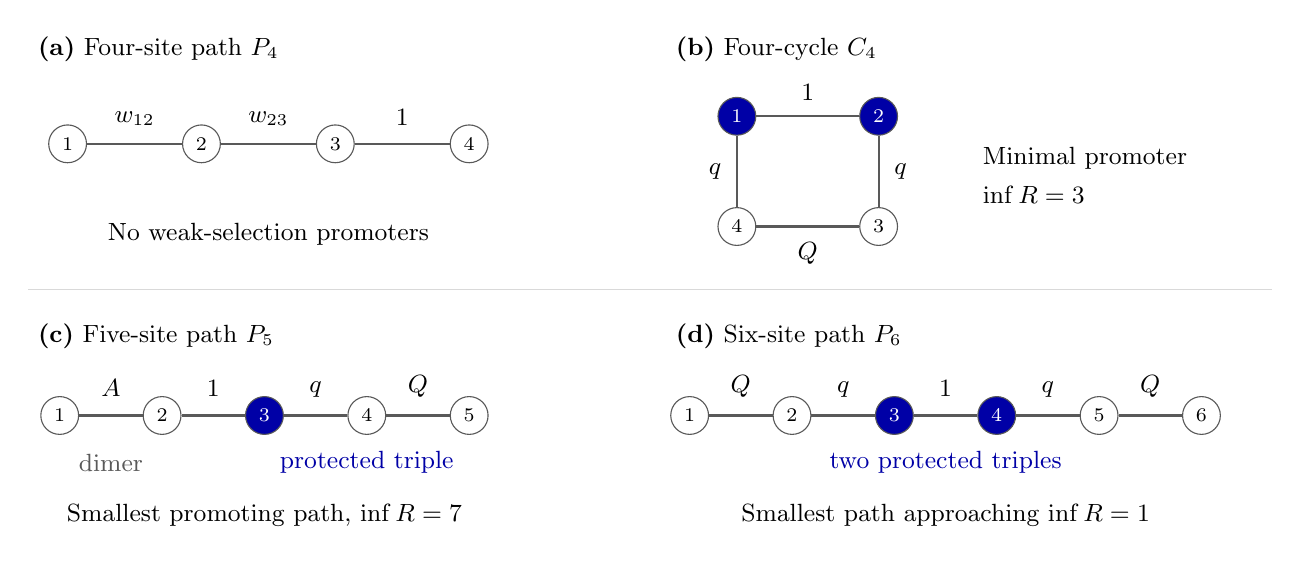
\begin{tikzpicture}[x=1cm,y=1cm,font=\small,
 site/.style={circle,draw=black!65,fill=white,minimum size=4.8mm,inner sep=0pt},
 pin/.style={site,fill=blue!65!black,text=white},
 edge/.style={draw=black!65,line width=.75pt}]
\node[anchor=west] at (0,2.8) {\textbf{(a)} Four-site path \(P_4\)};
\foreach \i/\x in {1/.5,2/2.2,3/3.9,4/5.6}
 {\node[site] (a\i) at (\x,1.6) {\scriptsize\i};}
\draw[edge] (a1)--node[above=3pt] {\(w_{12}\)}(a2);
\draw[edge] (a2)--node[above=3pt] {\(w_{23}\)}(a3);
\draw[edge] (a3)--node[above=3pt] {\(1\)}(a4);
\node at (3.05,.45) {No weak-selection promoters};
\node[anchor=west] at (8.1,2.8) {\textbf{(b)} Four-cycle \(C_4\)};
\node[pin] (b1) at (9,1.95) {\scriptsize1};
\node[pin] (b2) at (10.8,1.95) {\scriptsize2};
\node[site] (b3) at (10.8,.55) {\scriptsize3};
\node[site] (b4) at (9,.55) {\scriptsize4};
\draw[edge] (b1)--node[above=2pt] {\(1\)}(b2);
\draw[edge] (b2)--node[right=2pt] {\(q\)}(b3);
\draw[edge] (b3)--node[below=2pt] {\(Q\)}(b4);
\draw[edge] (b4)--node[left=2pt] {\(q\)}(b1);
\node[align=left,anchor=west] at (12,1.2) {Minimal promoter\\[3pt]\(\inf R=3\)};
\draw[black!15] (0,-.25)--(15.8,-.25);
\node[anchor=west] at (0,-.85) {\textbf{(c)} Five-site path \(P_5\)};
\foreach \i/\x in {1/.4,2/1.7,4/4.3,5/5.6}
 {\node[site] (c\i) at (\x,-1.85) {\scriptsize\i};}
\node[pin] (c3) at (3,-1.85) {\scriptsize3};
\draw[edge] (c1)--node[above=3pt] {\(A\)}(c2);
\draw[edge] (c2)--node[above=3pt] {\(1\)}(c3);
\draw[edge] (c3)--node[above=3pt] {\(q\)}(c4);
\draw[edge] (c4)--node[above=3pt] {\(Q\)}(c5);
\node[text=black!65] at (1.05,-2.45) {dimer};
\node[text=blue!65!black] at (4.3,-2.45) {protected triple};
\node at (3,-3.12) {Smallest promoting path, \(\inf R=7\)};
\node[anchor=west] at (8.1,-.85) {\textbf{(d)} Six-site path \(P_6\)};
\foreach \i/\x in {1/8.4,2/9.7,5/13.6,6/14.9}
 {\node[site] (d\i) at (\x,-1.85) {\scriptsize\i};}
\node[pin] (d3) at (11,-1.85) {\scriptsize3};
\node[pin] (d4) at (12.3,-1.85) {\scriptsize4};
\draw[edge] (d1)--node[above=3pt] {\(Q\)}(d2);
\draw[edge] (d2)--node[above=3pt] {\(q\)}(d3);
\draw[edge] (d3)--node[above=3pt] {\(1\)}(d4);
\draw[edge] (d4)--node[above=3pt] {\(q\)}(d5);
\draw[edge] (d5)--node[above=3pt] {\(Q\)}(d6);
\node[text=blue!65!black] at (11.65,-2.45) {two protected triples};
\node at (11.65,-3.12) {Smallest path approaching \(\inf R=1\)};
\path[use as bounding box] (0,-3.45) rectangle (16,3.05);
\end{tikzpicture}

\caption{Small supports distinguish establishment mechanisms.
All thresholds in this figure use uniform singleton introduction.
$P_4$ represents the paths with at most four sites that do not promote
at weak selection. $C_4$ is a minimal promoter, $P_5$ the smallest
promoting path, and $P_6$ the smallest path approaching threshold one.
Edge labels are relative weights; line thickness does not encode their
magnitude. Filled sites are dynamically protected pins, not fixed
external spins. The limits are $q\to\infty$, $q^2/Q\to0$ on $C_4$;
$1\ll q\ll A\ll Q$ on $P_5$; and $q\to\infty$, $q/Q\to0$ on
$P_6$. The six-site construction extends to every fixed longer path.}
\label{fig:paths}
\end{figure*}

The mathematics connects the local mechanism to a global result.
Grading the five-site response by outer contact degree identifies a
monotone improvement direction and determines the best threshold at
fixed inner ratio. On six sites, a positive polynomial bound forces
every near-barrier promoter into the protected-domain hierarchy.
Relations among its small ratios form a rank-one matrix. The resulting
toric coordinates control the response at the singular hierarchy limit,
allowing optimization over all positive weightings and proving that
the optimum is eventually exactly reflection symmetric.

The least six-site contact contrast is asymptotic to $656\epsilon^{-2}$ under uniform
introduction and $4050\epsilon^{-3}$ under birth-associated introduction
for a threshold $b/c=1+\epsilon$. Their different powers follow from
different leading monomials in the same exact response construction.
Under uniform introduction, further contrast can shorten an invasion,
but proximity to the minimum leaves little room for contact errors.
The constrained quadratic geometry determines this tolerance and an
exact waiting-time optimizer that persists at sufficiently small
selection. Nonlinear selection consumes the same margin, so the
improved threshold can coexist with a shrinking fixation advantage.
An optimal terminal-estimation bound connects that advantage to the
statistical time needed to resolve it.

Section~\ref{sec:model} defines the game and invasion experiment.
Sections~\ref{sec:response-theory} and \ref{sec:domains} derive the
response and domain mechanism. The support classification and global
contact design follow in Secs.~\ref{sec:classification} and
\ref{sec:cost}; time, tolerance and finite signal are developed in
Secs.~\ref{sec:v3-tolerance} and \ref{sec:v3-selection-window}.
Appendices~\ref{app:path-classification}--\ref{app:v3-joint-selection}
contain the threshold, establishment, optimization and observation-cost
proofs. Appendices~\ref{sec:physics} and \ref{app:v3-degree-closure}
develop the operator and response constructions;
Appendices~\ref{app:v4-toric}--\ref{app:v4-exact-time} give the toric,
convex-dual and neutral and selected exact-time arguments.
The preparation comparison and the payoff, encounter and support
extensions are proved in Appendices~\ref{app:v7-preparation} and
\ref{app:v7-robustness}.
\section{The game and the invasion experiment}
\label{sec:model}
We consider an inherited binary trait on a finite connected, loopless,
undirected graph. Each of its $N\ge2$ sites contains one individual,
with $n_i=1$ for cooperation and $n_i=0$ for defection. The distinction
between individual advantage and collective persistence begins with
the donation game.

\subsection{Payoffs and reciprocal contacts}
\label{sec:game}
A cooperative encounter costs the producer $c>0$ and benefits its
partner by $b\ge0$. The row player's payoff is
\begin{equation}
 \begin{array}{c|cc}
       & C & D\\ \hline
 C&b-c&-c\\
 D&b&0
 \end{array}
 \label{eq:donation-matrix}
\end{equation}
Microbial public-benefit production motivates this choice, although a
quantitative application would also need a specified transport and
uptake model~\cite{AllenGoreNowak2013}. Reciprocal weights satisfy
$w_{ij}=w_{ji}>0$ on edges and vanish off the support, including $w_{ii}=0$.
They define the site strengths and contact kernel,
\begin{equation}
 s_i=\sum_jw_{ij},\qquad P_{ij}=\frac{w_{ij}}{s_i},
 \qquad P\one=\one .
 \label{eq:kernel}
\end{equation}
We use the same kernel for averaged interactions and replacement,
\begin{equation}
 f_i(n)=-cn_i+b(Pn)_i,\qquad c>0,\quad b\ge0.
 \label{eq:payoff}
\end{equation}
Thus $(Pn)_i$ is the cooperative fraction among the encounters sampled by individual $i$.
At fixed neighboring traits, defection gains exactly $c$, since there
are no self-contacts. It is a strict best reply in every environment,
so all defection is the unique Nash equilibrium, the state in which
no individual gains by changing its own strategy, including mixed
strategies. Yet all cooperation gives everyone $b-c>0$ when $b>c$.
In the dynamics below, traits are inherited through copying; individuals
do not switch to their best reply. Their realized payoffs can differ
because their neighborhoods differ. Individual payoff dominance and population-level fixation advantage
therefore answer distinct questions about the same game.

The averaging convention matters on heterogeneous graphs. Accumulating
encounters gives $s_i f_i$, while distributing a donor's fixed benefit
budget uses the donor's normalization. These choices change the
selection criterion~\cite{McAvoyAllenNowak2020,McAvoyRaoHauert2021}.
\footnote{With distinct interaction and replacement kernels, neutral
ancestry follows replacement and the benefit contraction changes. The common-kernel bounds are extended to a specified mixed-encounter model in Sec.~\ref{sec:v7-robustness}.}

\subsection{Copying dynamics and physical time}
\label{sec:update}
Fecundity is $F_i=\phi(\delta f_i)>0$, with selection strength
$\delta\ge0$ and normalization $\phi(0)=\phi'(0)=1$ near
neutrality. We use $\phi(x)=1+x$ and $\phi(x)=e^x$.
A different positive slope-to-value ratio
rescales weak response without changing its threshold.
We write $r=b/c$ and $\kappa=\delta c$ for the dimensionless
benefit--cost ratio and selection intensity. Since $-c\le f_i\le b$,
the linear map is positive on every configuration precisely when
 $0\le\kappa<1$; the minimum $f_i=-c$ is attained by a lone
cooperator. The exponential map is positive for every finite $\kappa\ge0$.

At each global Poisson attempt, a source is chosen in proportion to
fecundity and its recipient through $P$. Writing $n^{j\leftarrow i}$
for the replaced configuration, the rates and backward generator are
\begin{align}
 r_{ij}(n)&=\frac{F_i(n)P_{ij}}{\sum_kF_k(n)},\label{eq:rates}\\
 (\mathcal A g)(n)&=\sum_{i,j}r_{ij}(n)
       [g(n^{j\leftarrow i})-g(n)] .
 \label{eq:backward}
\end{align}
Time is measured in global attempts, including copies between identical
traits; time in attempts per site is $t/N$.
Keeping the total attempt rate fixed makes contact designs comparable
at equal numbers of reproduction or copying opportunities. This is source-first
Birth--death updating. Choosing the recipient first and letting its
neighbors compete produces a different response
\cite{OhtsukiEtAl2006,AllenLippnerNowak2019}. Neutrality gives a weighted
invasion process. A fixed fitness for each type would describe constant
selection; here fecundity depends on the configuration through the game.

The process has an exact Doi--Peliti representation in the sector with
one particle per site~\cite{Doi1976SecondQuantization,Peliti1985PathIntegral}.
The two species label the alternative traits; $a_i^\dagger$ creates
a cooperative occupant and $d_i^\dagger$ a defective one, while
$a_i,d_i$ remove them. Introduce the number operators $\hat n_i^C=a_i^\dagger a_i$ and
$\hat n_i^D=d_i^\dagger d_i$, and restrict
$N_i=\hat n_i^C+\hat n_i^D=1$. Then
\begin{equation}
 \begin{aligned}
 B_{ij}^{\rm copy}&=\hat n_i^C(a_j^\dagger-d_j^\dagger)d_j
             +\hat n_i^D(d_j^\dagger-a_j^\dagger)a_j,\\
 \widehat{\mathcal L}&=\sum_{i\ne j}B_{ij}^{\rm copy}\widehat r_{ij}.
 \end{aligned}
 \label{eq:spin-generator}
\end{equation}
The diagonal rate acts before the conversion, as indicated by its
position on the right, and every term conserves each $N_i$.
Thus a physical initial state stays in the binary sector. The forward
generator obeys $\partial_t|p\rangle=\widehat{\mathcal L}|p\rangle$,
with $\widehat{\mathcal L}=\mathcal A^{\T}$ and stochastic Hamiltonian
$\mathcal H_{\rm st}=-\widehat{\mathcal L}$. This probability evolution
requires neither unitarity nor detailed balance
\cite{AlcarazEtAl1994,Schutz2001,DelRazoLammaMerbis2026}.
Appendix~\ref{sec:physics} gives the equivalent spin operator and the
sector projection needed in a coherent-state representation.

\subsection{Fixation, preparation and absorption time}
\label{sec:observables}
At positive weights, every mixed configuration eventually reaches
$\mathbf0$ or $\mathbf1$. Indeed, connectedness permits a sequence of
copies spreading either surviving type, so the finite mixed sector is
transient. Both consensus states are absorbing, although only defection
is a Nash equilibrium. The stationary measures are their convex
mixtures; copying cannot recreate an absent type.

Let $h_C(n)$ be the probability that the population eventually becomes
all cooperative when started from $n$. This fixation probability, also
called a committor in first-passage theory, satisfies
\begin{equation}
 \begin{gathered}
 \mathcal A h_C=0\quad\hbox{on mixed states},\\
 h_C(\mathbf0)=0,\qquad h_C(\mathbf1)=1.
 \end{gathered}
 \label{eq:committor}
\end{equation}
We compare two introduction experiments. One places a single cooperator
uniformly in an all-defector population; the other places a single
defector uniformly in an all-cooperator population. If $e_i$ has its
sole cooperator at $i$, their respective fixation probabilities are
\begin{equation}
 \rho_C=\frac1N\sum_i h_C(e_i),\quad
 \rho_D=\frac1N\sum_i[1-h_C(\one-e_i)].
 \label{eq:rho}
\end{equation}


Uniform placement chooses the site independently of its replacement
rate. Mutation arising during reproduction samples the recipient of a
copying event instead~\cite{McAvoyRaoHauert2021}. We will compare these
preparations on the same network and after separately optimizing the
network for each.

For a common, selection-independent distribution $\mu_i$ of introduction
sites, the averages in Eq.~\eqref{eq:rho} use $\mu_i$ in place of $1/N$.
The two preparations considered here are
\begin{equation}
 \mu_i^U=\frac1N,\qquad
 \mu_i^{\rm b}=\frac{T_i}{N},\qquad T_i=\sum_kP_{ki}.
 \label{eq:v7-preparation}
\end{equation}
The superscript $\mathrm b$ denotes birth-associated introduction.
In either homogeneous background every source has the same fecundity,
so the recipient of a birth has distribution $\mu^{\rm b}$ even at
finite selection. Superscripts identify the preparation when the
comparison requires it; unmarked quantities retain uniform preparation.
At neutrality both types have the same fixation probability
$\rho_0^\mu=\sum_i\mu_i\pi_i$, with the reproductive values $\pi_i$
defined in Eq.~\eqref{eq:reproductive}. This probability need not be $1/N$.


The invasion advantage is $\Delta=\rho_C-\rho_D$, and its weak
susceptibility is
\begin{equation}
 \mathcal S=\left.\partial_\delta\Delta\right|_{\delta=0}.
 \label{eq:response}
\end{equation}
For a cooperator introduced at a uniformly chosen site, let $\tau$ be
the absorption time and define
\begin{equation}
 T_U=\E[\tau],\qquad T_C=\E[\tau\mid C\text{ fixes}].
 \label{eq:times-definition}
\end{equation}
The unconditional mean includes extinction; the conditional mean counts
successful invasions. These definitions allow selection. We first solve the neutral-time problem
and then extend its optimizer to a stated range of selected dynamics in
Proposition~\ref{prop:v7-selected-time}. We say that the
network promotes cooperation when $\Delta>0$. This compares the two
traits against each other, whereas $\rho_C>1/N$ compares cooperative
invasion against neutral copying.

This ranking has a population interpretation under equal rare rates of
introducing the absent type at uniformly chosen sites. If each invasion
resolves before the next, the consensus populations communicate at
rates proportional to fixation probabilities, and
\begin{equation}
 X_C^{\rm rare}=\frac{\rho_C}{\rho_C+\rho_D},
 \qquad
 X_C^{\rm rare}>\frac12\ \Longleftrightarrow\ \Delta>0 .
 \label{eq:rare-abundance}
\end{equation}
The separation of introductions is taken at fixed weights and must be
checked again in a slow-absorption limit~\cite{McAvoyAllen2021}.

\section{Fluctuations and exact response}
\label{sec:response-theory}
The choice of observable is decisive. A common-density approximation
assigns every neighborhood the same cooperative fraction $x$, leaving
the payoff difference $(-c)$ and losing the mechanism for cooperative
fixation. We instead perturb the exact neutral process. Its conserved
coordinate turns the fixation response into an integral of correlations,
which close without an assumption of small fluctuations.

\subsection{The conserved coordinate and covariance response}
\label{sec:neutral-coordinate}\label{sec:absorbing-response}
For source-first copying, neutral fixation weights sites by inverse
strength rather than by their number,
\begin{equation}
 Z=\sum_i s_i^{-1},\qquad
 \pi_i=\frac{s_i^{-1}}Z,\qquad
 \Phi(n)=\sum_i\pi_i n_i .
 \label{eq:reproductive}
\end{equation}
The identity
\begin{equation}
 \pi_jP_{ij}=\pi_iP_{ji}
 =\frac{\gamma_{ij}}Z,\qquad
 \gamma_{ij}=\frac{w_{ij}}{s_is_j}
 \label{eq:edge-balance}
\end{equation}
makes the two copying directions cancel in $\mathcal A_0\Phi$.
Stopping this bounded martingale at consensus gives $h_C^0=\Phi$ and
$\rho_C^0=\rho_D^0=1/N$. Here $\pi_i$ is the neutral fixation probability of a singleton at $i$,
called its reproductive value. It differs from the strength-proportional
stationary measure of $P$. Ancestry follows a
received copy backward from $j$ to $i$, at rate $P_{ij}/N$
\cite{Maciejewski2014,SoodAntalRedner2008}.

Let $L_\gamma$ be the symmetric Laplacian with off-diagonal entries
$-\gamma_{ij}$. The first drift correction is
\begin{equation}
 \left.\partial_\delta\mathcal A\Phi(n)\right|_0
 =\frac{-c\,n^\T L_\gamma n+
               b(Pn)^\T L_\gamma n}{NZ}.
 \label{eq:drift}
\end{equation}
The derivative of the global rate normalization cancels because it
multiplies $\mathcal A_0\Phi=0$. The two terms separate the cost contribution to fixation drift across
trait interfaces from the benefit due to different cooperative environments,
\begin{equation}
 n^\T L_\gamma n=\sum_{i<j}\gamma_{ij}(n_i-n_j)^2>0.
 \label{eq:dirichlet}
\end{equation}
\begin{equation}
 (Pn)^\T L_\gamma n=
 \sum_{i<j}\gamma_{ij}(n_i-n_j)[(Pn)_i-(Pn)_j].
 \label{eq:benefit}
\end{equation}
The first is strictly positive on mixed configurations and penalizes
interfaces. The second compares cooperative environments across each
interface; its sign depends on the correlations generated by copying.

Writing $h_C=\Phi+\delta h_1+O(\delta^2)$,
$\mathcal A_1=\partial_\delta\mathcal A|_{\delta=0}$ and
$j=\mathcal A_1\Phi$, the absorbing Dirichlet problem gives
\begin{equation}
 h_1=(-\mathcal A_{0,\mathrm{mix}})^{-1}j
 =\int_0^\infty e^{t\mathcal A_{0,\mathrm{mix}}}j\,dt .
 \label{eq:absorbing-susceptibility}
\end{equation}
The restriction to mixed states stops each history at consensus. Its
Green function in Eq.~\eqref{eq:absorbing-susceptibility} integrates
the selection drift over precisely that transient part of the evolution. Write $\E_\delta$ for expectation at
selection strength $\delta$ with a uniformly placed cooperative singleton.
At neutrality, $\E_0[n_i(t)]=1/N$ at every site and time. Nevertheless,
the covariance $C_{ij}(t)=\E_0[n_i(t)n_j(t)]-\E_0[n_i(t)]\E_0[n_j(t)]$
evolves, and
\begin{equation}
 \left.\partial_\delta\frac{d}{dt}\E_\delta[\Phi(n(t))]\right|_0
 =\frac{\operatorname{Tr}[(bP^\T L_\gamma-cL_\gamma)C(t)]}{NZ}.
 \label{eq:covariance}
\end{equation}
The mean contribution cancels by $P\one=\one$ and $L_\gamma\one=0$.
Thus the neutral mean density is stationary while correlations carry
the response. This is the fluctuation mechanism missed by the
common-density approximation. Weak selection controls the perturbation
of rates; the neutral fluctuations themselves are treated exactly.

\subsection{Ancestral pairs and the invasion threshold}
\label{sec:pair-response}
The integrated disagreement
\begin{equation}
 D_{ij}=\int_0^\infty\E_0[(n_i(t)-n_j(t))^2]\dd t,\qquad D_{ii}=0
 \label{eq:disagreement}
\end{equation}
has a direct ancestral interpretation. Trace each received copy back
to its source. Two such lineages move independently until they meet
and share one ancestor. Before that meeting, uniform singleton
preparation makes their disagreement probability $2/N$, so
$D_{ij}=(2/N)\E_{ij}[\tau_{\rm meet}]$. Consequently
\begin{equation}
 (T_i+T_j)D_{ij}
 -\sum_k(P_{ki}D_{kj}+P_{kj}D_{ik})=2,\quad i\ne j,
 \label{eq:pair-system}
\end{equation}
where $T_i=\sum_kP_{ki}$ and $T_i/N$ is the neutral overwrite rate.
This replaces $2^N-2$ transient configuration unknowns by
$\binom N2$ ancestral pairs. The source two includes both preparation
and clock normalization
\cite{AllenEtAl2017,AllenEtAl2021,McAvoyAllen2021}.
Contracting this solution with the drift forms defines
\begin{equation}
 \begin{gathered}
 \mathsf B=\tfrac12(P^\T L_\gamma+L_\gamma P),\\
 K=\sum_{i<j}\gamma_{ij}D_{ij},\qquad
 J=-\sum_{i<j}\mathsf B_{ij}D_{ij}.
 \end{gathered}
 \label{eq:JK}
\end{equation}
The symmetric benefit matrix $\mathsf B$ has zero row sums. Complementary preparations
have the same first-order drift, hence
\begin{equation}
 \mathcal S=\frac{2}{NZ}(bJ-cK).
 \label{eq:criterion}
\end{equation}
Equivalently, $\mathcal S=b\chi_b-c\chi_c$, with
$\chi_b=2J/(NZ)$ and $\chi_c=2K/(NZ)>0$. For $J>0$,
\begin{equation}
 R(w)=K/J,\qquad \mathcal S>0\ \Longleftrightarrow\ b/c>R(w).
 \label{eq:threshold}
\end{equation}
If $J\le0$, nonnegative benefit cannot compensate positive cost at
first order. A positive susceptibility ensures positive advantage at
sufficiently small selection for fixed weights; this interval can
shrink as the contact ratios become singular.


Changing preparation leaves the ancestral-pair matrix unchanged and
changes its source. In place of Eq.~\eqref{eq:pair-system},
\begin{equation}
 (T_i+T_j)D_{ij}^{\mu}
 -\sum_k(P_{ki}D_{kj}^{\mu}+P_{kj}D_{ik}^{\mu})
 =N(\mu_i+\mu_j).
 \label{eq:v7-pair-preparation}
\end{equation}
Indeed, if two ancestors occupy distinct sites $k,l$ at time zero,
a singleton drawn from $\mu$ makes them disagree with probability
$\mu_k+\mu_l$. The killed pair resolvent integrates this source.
For birth-associated introduction the right side is $T_i+T_j$;
the resulting $D_{ij}^{\rm b}$ is the expected number of ancestral
jumps before meeting, including the final coalescing jump. Uniform
introduction instead weights elapsed meeting time. The contractions
in Eq.~\eqref{eq:JK} and the criterion in Eq.~\eqref{eq:criterion}
retain their form with $D^{\mu},K^{\mu},J^{\mu}$. Preparation thus
changes which histories enter the response, even when the copying
generator is held fixed.


\subsection{Filtered observables and higher response}
\label{sec:v4-observable-algebra}
The threshold uses a pair response, but its observable advantage at
finite selection also depends on higher orders. We organize these
orders before calculating the shrinking selection window in
Sec.~\ref{sec:v3-selection-window}. With $\sigma_i=2n_i-1$,
polynomials agreeing on all binary configurations are identified in
\begin{equation}
 \mathscr A_N=\mathbb R[n_1,\ldots,n_N]/(n_i^2-n_i)
 =\mathbb R[\sigma_1,\ldots,\sigma_N]/(\sigma_i^2-1).
 \label{eq:v4-boolean}
\end{equation}
The quotient imposes the relations $n_i^2=n_i$, or $\sigma_i^2=1$.
Squarefree spin monomials $\sigma_S=\prod_{i\in S}\sigma_i$ form a
basis and multiply as $\sigma_S\sigma_T=\sigma_{S\triangle T}$,
where $S\triangle T$ is the symmetric difference of the index sets.
Degree is therefore a filtration rather than a grading.  Repeated indices
can lower it. Let $\mathscr F_k$ contain degrees at most $k$, with
$\mathscr F_{-1}=0$. The associated graded algebra separates successive
degrees, retaining only the leading degree of each product,
\begin{equation}
 \begin{gathered}
 \gr\mathscr A_N=\bigoplus_{k=0}^N\mathscr F_k/\mathscr F_{k-1},\\
 \gr\mathscr A_N\simeq
 \mathbb R[x_1,\ldots,x_N]/(x_1^2,\ldots,x_N^2),\\
 H_{\gr\mathscr A_N}(t)=(1+t)^N.
 \end{gathered}
 \label{eq:v4-hilbert-full}
\end{equation}
The coefficient of the formal variable $t^k$ counts independent
degree-$k$ observables. This Hilbert series agrees with the exterior
algebra count, but the variables here commute and introduce no fermionic
signs.

Neutral copying preserves $\mathscr F_k$. A donation payoff is linear, so each
selection insertion raises degree by at most one. Centering it as
$\xi_i=[-c\sigma_i+b(P\sigma)_i]/2$ removes a common fecundity
factor. In the coordinate $u_c=\delta/[1+\delta(b-c)/2]$ for linear
fecundity and $u_c=\delta$ for exponential fecundity,
$h_C=\Phi+\sum_{m\ge1}u_c^m h_m$ obeys
\begin{equation}
 \begin{gathered}
 \deg h_m\le\min(N,m+1),\\
 h_m(-\sigma)=(-1)^{m+1}h_m(\sigma),\quad m\ge1.
 \end{gathered}
 \label{eq:v4-degree-response}
\end{equation}
The zero-boundary neutral inverse preserves these spaces.
Appendix~\ref{app:v3-degree-closure} proves the induction and the
corresponding timed response.

For a reflection-symmetric six-site problem, averaging the identity and
reflection actions counts invariant monomials. A reflection-fixed subset
is a union of mirrored pairs, giving
\begin{equation}
 \begin{aligned}
 H_{\rm refl}(t)&=\frac{(1+t)^6+(1+t^2)^3}{2}\\
 &=1+3t+9t^2+10t^3
 +9t^4+3t^5+t^6.
 \end{aligned}
 \label{eq:v4-reflected-hilbert}
\end{equation}
The degree bound and one independent consensus condition per parity
sector leave $1+9-1=9$, $3+10-1=12$, and $1+9+9-1=18$ response
coefficients at orders one, two, and three, instead of 62 mixed-state
unknowns. Without reflection the first response uses fifteen pairs.
Their disagreements $d_{ij}=(1-\sigma_i\sigma_j)/2$ satisfy
\begin{equation}
 d_{ij}^2=d_{ij},\qquad
 2d_{ij}d_{jk}=d_{ij}+d_{jk}-d_{ik}.
 \label{eq:v4-pair-relations}
\end{equation}
Thus higher-order closure follows from the binary algebra rather than
from factorization of correlations.

On paths and cycles, nearest-neighbor ancestry also simplifies the
propagator. A change of basis mixing each correlation with lower-degree
ones absorbs the terms in which two ancestral indices meet. In this
basis, propagation is built from one-particle evolution and its
antisymmetrized products, or exterior powers. The pair response
then satisfies $B_eX+XB_e^{\T}=-J_{\rm src}$, a skew Sylvester equation
for the antisymmetric pair coefficients $X$ and source $J_{\rm src}$.
In a one-particle eigenbasis, inversion uses sums of one-particle
eigenvalues instead of a separate dense pair inverse.
Here $B_e$ is the one-particle matrix used to propagate the correlation
sector even under trait complementation. On a cycle its wrap-edge sign is reversed,
an antiperiodic boundary condition. The derivation and the
physical-clock insertions are in Appendices~\ref{app:v3-neutral-cas}
and \ref{app:v3-sylvester-time}. These auxiliary fermions act on
coefficients; the microscopic probabilities remain those of the binary
copying process.


Symbolic calculations were performed using the open-source computer
algebra systems SageMath and SymPy, with Gr\"obner-basis and Hilbert-series
checks in Singular~\cite{SageMathSoftware,SymPySoftware,SingularSoftware}.
The rational-function solutions, polynomial identities and coefficient-sign
checks underlying the threshold and optimization results were computed
using exact integer or rational arithmetic. Independent reconstructions
from the microscopic generators and high-precision numerical evaluations
checked the finite-parameter expressions. The asymptotic estimates and
their domains of validity are derived in the text and appendices.


\section{Formation and competition of protected domains}
\label{sec:domains}
We now evaluate the response in a limit where persistent domains emerge.
The reduction must determine both their competition and the probability
that a singleton reaches that stage.

\subsection{Protection from normalized reciprocal contacts}
\label{sec:protected-mechanism}
Number the path consecutively and choose
\begin{equation}
 \begin{gathered}
 (w_{12},w_{23},w_{34},w_{45},w_{56})=(Q,q,1,q,Q),\\
 u=q^{-1},\qquad v=q/Q,\qquad (u,v)\longrightarrow(0,0).
 \end{gathered}
 \label{eq:p6-weights}
\end{equation}
A central site sends fractions $1/(1+u)$ toward its followers and
$u/(1+u)$ across the bridge. Its adjacent follower sends only
$v/(1+v)$ back toward it because the outer edge $Q$ dominates that
follower's transmissions. Reciprocal contacts therefore produce
directed influence after normalization.
Both incoming overwrite channels of a central site are weak, although
that site transmits efficiently to its followers. Consistently, the reproductive
values in Eq.~\eqref{eq:reproductive} tend to $1/2$ at each central site and
to zero at the followers. Protection refers to this dynamical
asymmetry, not to an imposed difference between the two traits.

At $u=v=0$, sites 3 and 4 retain their traits while their followers
align. We call these sites \emph{pins}; they can change at finite
positive weights. Denote the four aligned states by their domain traits
$00,10,01,11$. A pin introduction establishes its triple with probability
tending to one, while a follower introduction disappears. Uniform
placement leaves mass $1/6$ in each mixed domain and loses $2/3$
during formation, as shown in Fig.~\ref{fig:domains}.
\begin{figure*}[t]
\centering

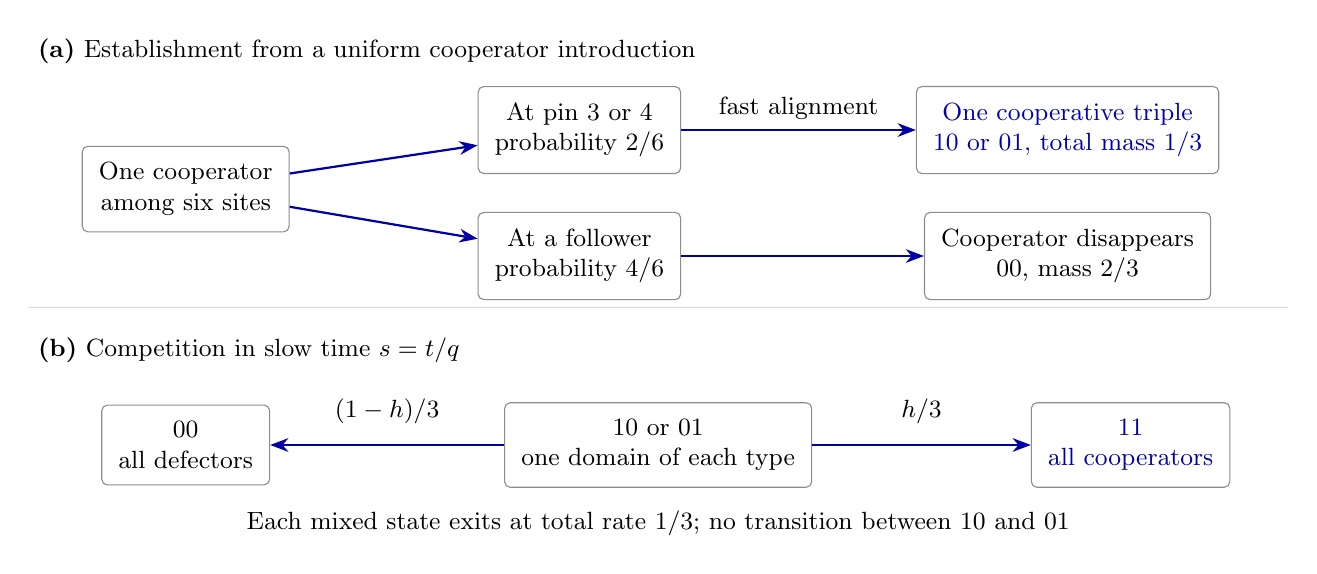
\begin{tikzpicture}[x=1cm,y=1cm,font=\small,>=Stealth,
 box/.style={draw=black!45,rounded corners=2pt,align=center,inner sep=6pt},
 rate/.style={->,line width=.8pt,draw=blue!65!black}]
\node[anchor=west] at (0,3.0) {\textbf{(a)} Establishment from a uniform cooperator introduction};
\node[box] (start) at (2,1.25) {One cooperator\\among six sites};
\node[box] (pin) at (7,2) {At pin 3 or 4\\probability \(2/6\)};
\node[box] (fol) at (7,.4) {At a follower\\probability \(4/6\)};
\node[box,text=blue!65!black] (mixed) at (13.2,2) {One cooperative triple\\\(10\) or \(01\), total mass \(1/3\)};
\node[box] (zero) at (13.2,.4) {Cooperator disappears\\\(00\), mass \(2/3\)};
\draw[rate] (start)--(pin);
\draw[rate] (start)--(fol);
\draw[rate] (pin)--node[above] {fast alignment}(mixed);
\draw[rate] (fol)--(zero);
\draw[black!15] (0,-.25)--(16,-.25);
\node[anchor=west] at (0,-.8) {\textbf{(b)} Competition in slow time \(s=t/q\)};
\node[box] (dd) at (2,-2) {\(00\)\\all defectors};
\node[box] (mid) at (8,-2) {\(10\) or \(01\)\\one domain of each type};
\node[box,text=blue!65!black] (cc) at (14,-2) {\(11\)\\all cooperators};
\draw[rate] (mid)--node[above=4pt] {\((1-h)/3\)}(dd);
\draw[rate] (mid)--node[above=4pt] {\(h/3\)}(cc);
\node at (8,-3) {Each mixed state exits at total rate \(1/3\); no transition between \(10\) and \(01\)};
\path[use as bounding box] (0,-3.25) rectangle (16,3.3);
\end{tikzpicture}

\caption{The initial individual and the eventual domain competitor.
The upper panel distinguishes pin introductions, which establish an
aligned triple in the hierarchy limit, from follower introductions,
which disappear. The lower panel is the resulting four-state process
in slow time $s=t/q$; its arrows are rates in that clock.
Here $h$ is the probability that cooperation wins the domain contest. The entrance
weights belong to the original uniform-singleton experiment. A pin is
slowly overwritten, not externally fixed at finite weights.}
\label{fig:domains}
\end{figure*}
A cooperative triple has leading payoff $b-c$ at each site and a
defective triple has payoff zero. A rare bridge copy changes a pin;
its followers usually align before the next rare copy. The collective advantage $b-c$ is therefore realized only after
establishment. The effective competitors are assembled by the
individual copying rules, with no separate rule for group reproduction.

\subsection{Eliminating fast configurations}
\label{sec:effective-memory}
Partition the forward generator $\mathsf Q=\mathcal A^{\T}$ into
the four aligned states $S$ and the remaining 60 configurations $F$.
For $\operatorname{Re}z>0$, let
$\widetilde p_S(z)=\int_0^\infty e^{-zt}p_S(t)\,dt$.
Their exact Laplace-space elimination gives
\begin{align}
 \Sigma(z)&=\mathsf Q_{SF}(zI-\mathsf Q_{FF})^{-1}
                    \mathsf Q_{FS},\notag\\
 \bigl[zI-\mathsf Q_{SS}-\Sigma(z)\bigr]\widetilde p_S(z)
 & =p_S(0) \label{eq:main-self-energy}\\
 &\quad+\mathsf Q_{SF}(zI-\mathsf Q_{FF})^{-1}p_F(0). \notag
\end{align}
The self-energy $\Sigma(z)$ sums excursions through fast configurations,
including their duration. The source on the right is equally necessary.
It determines how the original singleton enters the domain process,
rather than assuming that an aligned domain was present initially. At zero frequency the corresponding backward operator is
\begin{equation}
 L_{\rm harm}
 =\mathsf A_{SS}-\mathsf A_{SF}\mathsf A_{FF}^{-1}\mathsf A_{FS}
 =u[L_0+O(u+v)] ,
 \label{eq:schur}
\end{equation}
where $\mathsf A_{XY}$ are blocks of the backward generator. It computes hitting
probabilities, while physical times also require a differentiated
resolvent or the equivalent corrected Poisson source. The time-domain
memory equation is derived in Appendix~\ref{app:p6-protected}.

The slow limit is uniform on compact positive-fecundity domains. A fixed
sequence of follower-aligning copies bounds the fast inverse, and every
row leaving $S$ contains an exact factor $u$.  At $u=0$ the aligned
domains are closed for all nearby $v$. Dividing out this factor leaves
an $O(u+v)$ error, with no additional assumption $v\ll u$
\cite{SlowAvrachenkovHaviv2004}.

\subsection{Fixation and first-passage distributions}
\label{sec:finite-selection}\label{sec:domain-times}
Set $a=\phi(\delta(b-c))$, $d_0=\phi(0)=1$ and $h=a/(a+d_0)$.
The total leading fecundity in a mixed aligned state is $3(a+d_0)$,
so the generator in slow time $s=t/q$ is
\begin{equation}
 L_0=\frac13
 \begin{pmatrix}
 0&0&0&0\\
 1-h&-1&0&h\\
 1-h&0&-1&h\\
 0&0&0&0
 \end{pmatrix}
 \quad (00,10,01,11).
 \label{eq:domain-generator}
\end{equation}
Each mixed state has exit rate $1/3$ and cooperative exit probability
$h$. Including the entrance masses,
\begin{align}
 \rho_C&=\frac h3+O(u+v),&
 \rho_D&=\frac{1-h}{3}+O(u+v),\notag\\
 \Delta&=\frac{a-d_0}{3(a+d_0)}+O(u+v).
 \label{eq:p6-selected}
\end{align}
These errors are uniform on compact positive-fecundity domains for
locally Lipschitz $\phi$. A fixed $b>c$ therefore gives positive
limiting advantage at fixed positive selection for strictly increasing
fecundity. In particular,
\begin{equation}
 \Delta_\infty=
 \begin{cases}
 \displaystyle\frac{\delta(b-c)}{3[2+\delta(b-c)]}\,,
       &\phi(x)=1+x,\\[2mm]
 \displaystyle\frac13\tanh\!\frac{\delta(b-c)}2\,,
       &\phi(x)=e^x.
 \end{cases}
 \label{eq:selected-maps}
\end{equation}
The linear map must remain positive in establishment configurations as
well as aligned ones. At weak selection, $\mathcal S\to(b-c)/6$.

The same entrance probabilities and holding rate give
\begin{equation}
 T_U=q[1+O(u+v)],\qquad
 T_C=3q[1+O(u+v)] .
 \label{eq:p6-times}
\end{equation}
For every $s>0$,
\begin{align}
 \Pr(\tau/q>s)&\longrightarrow\tfrac13e^{-s/3},\notag\\
 \Pr(\tau/q>s\mid C\text{ fixes})&\longrightarrow e^{-s/3}.
 \label{eq:p6-tails}
\end{align}
The limiting unconditional distribution assigns probability $2/3$
to zero, because the formation transient is compressed to zero on the slow clock.


Conditioning on extinction retains both fast failed introductions
and unsuccessful domain competitors. Their survival probability and
mean are
\begin{equation}
 \begin{gathered}
 \Pr(\tau/q>s\mid C\text{ becomes extinct})\\
 \longrightarrow\frac{1-h}{3-h}e^{-s/3},\quad s>0,\\
 T_{\rm ext}^C=\frac{3(1-h)}{3-h}q+O(1+q^2/Q).
 \end{gathered}
 \label{eq:v7-extinction-time}
\end{equation}
The atom at zero has weight $2/(3-h)$. At neutrality the mean is
$3q/5$ to leading order, compared with $3q$ for successful fixation.
Subtracting the successful subdistribution from the unconditional
one proves the limit; the time resolvent controls the mean error.


In the slow limit, successful invasions have an exponential waiting
time. The additive finite-weight correction to the mean is $O(1+q^2/Q)$, bounded when $Q$ is at least of order
$q^2$. Appendix~\ref{app:p6-protected} also gives the full limiting
propagator and multivariate occupation generating function.

The rare-introduction abundance tends to $h$ when introductions of
total rate $\nu$ remain separated, $\nu q\ll1$. Figure~\ref{fig:finite}
compares the reduction with the finite microscopic equations. When
$b/c-1$ is comparable to $u+v$, formation corrections determine the
sign; Sec.~\ref{sec:v3-selection-window} calculates this regime.
\begin{figure*}[t]
\centering
\includegraphics[width=.9\textwidth]{figures/finite_response.pdf}
\caption{Finite microscopic checks on $(q^3,q,1,q,q^3)$.
(a) The complete committor calculation for exponential fecundity at
$\kappa=\delta c=0.25$, compared with the limiting advantage
$\tfrac13\tanh[\kappa(b/c-1)/2]$.
(b) Neutral mean absorption times approach $T_U/q=1$ and $T_C/q=3$.
The two panels test selected fixation and neutral time separately.
This family illustrates the mechanism; the optimal contact design is
determined below.}
\label{fig:finite}
\end{figure*}

\section{Sharp thresholds and the role of support}
\label{sec:classification}
The domain construction approaches $b/c=1$. A support-independent
obstruction proves that this is the lowest possible threshold. Smaller
supports test which parts of domain formation are necessary to reach it.

\subsection{A universal barrier and longer paths}
\label{sec:universal-bound}\label{sec:long-domains}
At finite selection the neutral fixation coordinate has drift
\begin{equation}
 \mathcal A\Phi=
 \frac{\sum_{i<j}(\gamma_{ij}/Z)
        [F_i-F_j](n_i-n_j)}{\sum_kF_k}.
 \label{eq:supermartingale}
\end{equation}
For $0\le b\le c$ on a discordant edge with $n_i=1,n_j=0$,
\begin{equation}
 f_i-f_j\le -(c-b)-b(P_{ij}+P_{ji})<0.
 \label{eq:edge-obstruction}
\end{equation}
Strictly increasing fecundity therefore makes $\Phi$ a strict
supermartingale up to absorption, and optional stopping gives
\begin{equation}
 \rho_C<1/N<\rho_D,\qquad 0\le b\le c,\quad\delta>0.
 \label{eq:finite-no-go}
\end{equation}
The same edge estimate gives a quantitative weak-selection obstruction,
\begin{equation}
 \begin{gathered}
 X_{\rm e}=\sum_{i<j}\gamma_{ij}(P_{ij}+P_{ji})D_{ij},\\
 K-J\ge X_{\rm e}>0,\qquad
 R-1\ge\frac{X_{\rm e}}{K-X_{\rm e}}\quad(J>0).
 \end{gathered}
 \label{eq:edge-gap-bound}
\end{equation}
Here $X_{\rm e}/K$ averages the sum of the two directional copying
probabilities with weights proportional to $\gamma_{ij}D_{ij}$.
Approaching $R=1$ therefore requires these weighted disagreement
histories to concentrate on edges with weak copying in both directions.
Appendix~\ref{app:path-universal-barrier} derives the bound and the
stopping argument. The finite-selection obstruction needs strictly
increasing fecundity; its strict first-order response also requires
$\phi'(0)>0$.

Two protected domains approach $R=1$ on every fixed path with
$N\ge6$ sites. For $m_L,m_R\ge2$, $N=m_L+m_R+2$, choose
\begin{equation}
 (\underbrace{q^3,\ldots,q^3}_{m_L-1},q,1,q,
        \underbrace{q^3,\ldots,q^3}_{m_R-1}).
 \label{eq:long-path}
\end{equation}
The domain sizes are $m_L+1$ and $m_R+1$. Their holding times may
differ, but each cooperative exit probability is $h=a/(a+d_0)$ and
each pin is introduced with probability $1/N$. Thus
\begin{equation}
 \begin{gathered}
 \rho_C=\frac{2h}{N}+O(q^{-1}),\qquad
 \rho_D=\frac{2(1-h)}N+O(q^{-1}),\\
 \mathcal S\longrightarrow\frac{b-c}{N},
 \end{gathered}
 \label{eq:long-path-law}
\end{equation}
with $T_U=q+O(1)$ and $T_C=Nq/2+O(1)$.
Appendix~\ref{app:path-general-times} derives the unequal-domain
distributions and variances. Here $N$ is fixed before the weight limit;
the error constants need not be uniform in $N$. Setting a weak link
to zero first would create extra closed classes.

\begin{proposition}[Sharp path thresholds]
\label{thm:path-classification}
For the common-kernel averaged donation game and paired uniform
singleton preparation, the infimum over positive weights with $J>0$ is
\begin{equation}
 R_*(P_N)=
 \begin{cases}
 +\infty,&2\le N\le4,\\
 7,&N=5,\\
 1,&N\ge6.
 \end{cases}
 \label{eq:path-classification}
\end{equation}
The infinite value denotes an empty promoter set. Every finite value
is strict and unattained at finite positive weights, with $N$ fixed
before the limit.
\end{proposition}
\begin{proof}
The supermartingale bound and protected-domain
construction settle $N\ge6$. The smaller-path signs and the five-site
bound below complete the classification; their proofs are in
Appendices~\ref{app:path-small}--\ref{app:path-p5-sharpness}.
\end{proof}

\subsection{The four-cycle and the five-site establishment penalty}
\label{sec:small-supports}\label{sec:five-site-mechanism}
For at most three sites every mixed state is a singleton or its
complement, with adverse benefit drift
\begin{equation}
 (Pe_k)^\T L_\gamma e_k
 =-\sum_{i\ne k}P_{ik}\gamma_{ik}<0.
 \label{eq:small-benefit}
\end{equation}
Solving the six pair equations on $P_4$ gives a negative site-resolved
benefit coefficient $J_\ell$ for every singleton placement $\ell$
(Appendix~\ref{app:path-small}). The other four-site tree, the star, has pointwise nonpositive
benefit drift. Their signs are derived in
Appendices~\ref{app:path-small} and \ref{app:resource-comparison}.

Closing $P_4$ into $C_4$ changes the cooperative environment. In the
cycle $(1,q,Q,q)$, with $q\to\infty$ and $q^2/Q\to0$, two pins
influence a shared strongly coupled pair. With opposing neutral pins,
this pair visits $(0,0),(0,1),(1,1)$ with equal stationary weights.
The threshold tends to three, and the global inequality in
Sec.~\ref{sec:cost-comparison} proves its sharpness. Thus $C_4$ is
minimal in both sites and edges among simple loopless undirected
promoting supports.

The five-site path $(A,1,q,Q)$ places a dimer beside a protected triple.
Take $u=1/q\to0$, $v=q/Q\to0$ at fixed $\eta=q/A>0$.
A cooperator introduced in the dimer first contests payoffs $(-c)$ and $b$,
so its establishment probability is
\begin{equation}
 p_C=\frac{\phi(-\delta c)}
 {\phi(-\delta c)+\phi(\delta b)},\qquad p_D=1-p_C .
 \label{eq:dimer-establishment}
\end{equation}
At neutrality $p_C=1/2$ and $p_C'(0)=-(b+c)/4$. This adverse
establishment response competes with the $b-c$ advantage of an aligned
cooperative domain. For $a=\phi(\delta(b-c))$, $d_0=\phi(0)$, the
left- and right-cooperative domain committors are
\begin{equation}
 h_L=\frac{\eta a}{\eta a+d_0 p_D},\qquad
 h_R=\frac{a p_C}{a p_C+\eta d_0}.
 \label{eq:dimer-slow-h}
\end{equation}
The factors $p_C,p_D$ enter again when a rare copy converts an existing
dimer. Including uniform preparation,
\begin{align}
 \rho_C&\longrightarrow\tfrac25p_Ch_L+\tfrac15h_R,\notag\\
 \rho_D&\longrightarrow\tfrac25p_D(1-h_R)+\tfrac15(1-h_L),
 \label{eq:dimer-rho}
\end{align}
and therefore
\begin{equation}
 \mathcal S\longrightarrow
 \frac{2\eta}{5(1+2\eta)^2}
 [(1-2\eta)b-(7+2\eta)c].
 \label{eq:dimer-response}
\end{equation}
The limiting threshold is $(7+2\eta)/(1-2\eta)$ for $0<\eta<1/2$;
the benefit coefficient vanishes at $\eta=1/2$ and becomes adverse
above it. Letting $\eta\to0$ approaches seven but also suppresses
the amplitude. The controlled expansion is
\begin{equation}
 \mathcal S=\frac{2\eta}{5}(b-7c)
           +O(\eta u+\eta^2+v),
 \label{eq:dimer-uniform}
\end{equation}
coefficientwise in $b,c$. The ordering $1\ll q\ll A\ll Q$ makes
the remainder relatively small. 

A pin introduction alone has leading paired threshold three. Indeed,
differentiating the two singleton committors in
Eq.~\eqref{eq:dimer-rho} gives
\begin{equation}
 \begin{aligned}
 \left.\partial_\delta(p_Ch_L)\right|_0
 &=-\frac{\eta[\eta(b+c)+2c]}{(1+2\eta)^2},\\
 \left.\partial_\delta h_R\right|_0
 &=\frac{\eta(b-3c)}{(1+2\eta)^2}.
 \end{aligned}
 \label{eq:p5-site-cancellation}
\end{equation}
There are two dimer sites. Their adverse responses shift the leading
uniform threshold from three to seven even though the protected pin
already favors cooperative invasion when $b>3c$.


\subsection{Outer grading and the exact five-site envelope}
\label{sec:v4-p5-grading}
The dimer calculation explains how seven is approached. To prove that
no other weighting does better, we organize the exact ten-pair solution
as $R=U/V$ after clearing a positive denominator. Then $U>0$
and $\operatorname{sgn}V=\operatorname{sgn}J$. Grading these
polynomials by total degree in the outer weights $A,Q$ gives
\begin{equation}
 \begin{gathered}
 U=\sum_{m=0}^{15}U_m,\quad V=\sum_{m=0}^{15}V_m,
 \\
 U_m\ge0,\quad V_m<0\ (m<15).
 \end{gathered}
 \label{eq:v4-p5-grades}
\end{equation}
The cost numerator can be written as a sum over directed forests of
the ancestral pair-state graph, with paths ending at specified roots. Each
forest contributes a product of positive rates; counting the possible
outgoing rows proves the nonnegative cost grades after denominators
are cleared. The negative benefit grades follow from a
finite polynomial identity; $(-V_{14})$ is a square term plus a
positive-coefficient polynomial. The precise
normalization and identities are in Appendix~\ref{app:path-classification}.

Under $(A,Q)\mapsto(\ell A,\ell Q)$, the scaled polynomials
$\ell^{-15}U(\ell A,q,\ell Q)$ and
$\ell^{-15}V(\ell A,q,\ell Q)$ are nonincreasing and strictly
increasing, respectively.
Hence every promoter
improves strictly along its outer ray,
\begin{equation}
 \frac{d}{d\ell}R(\ell A,q,\ell Q)<0.
 \label{eq:v4-p5-ray}
\end{equation}
A ray has a unique onset if $V_{15}>0$ and never promotes otherwise.
The top-degree difference has a positive factorization, which together
with the lower-grade signs proves $U-7V>0$ for all positive weights.

The same outer-ray limit gives the exact envelope at fixed inner ratio.
Reverse the path if necessary so that $q\ge1$, and define
\begin{equation}
 D_5(q)=11q^4-16q^3-124q^2-128q-33.
 \label{eq:v4-p5-inner-polynomial}
\end{equation}
Promoting outer weights exist exactly when $q>q_c$, the unique
positive root $q_c=4.536774892089\ldots$ of $D_5$. For these $q$,
\begin{equation}
 \begin{aligned}
 \mathcal R_5(q)&=\inf_{A,Q>0,J>0}R(A,1,q,Q)\\
 &=\frac{2(q+1)^2(11q^2+28q+11)(7q+10)}{(2q+3)D_5(q)}.
 \end{aligned}
 \label{eq:v4-p5-envelope}
\end{equation}
After a common positive factor is removed, the top-degree quotient is
fractional-linear and increasing in $A/Q$. Its boundary value gives
this envelope, approached by $(A,Q)=(L,L^2)$ as $L\to\infty$.
It decreases from infinity to seven, with
$\mathcal R_5(q)=7+83/(2q)+O(q^{-2})$.
Proposition~\ref{v4:prop:p5-envelope} proves the monotonicity and
controlled limit. At finite contrast the outer ray reaches the cap;
optimizing the two remaining ratios is a separate problem.


\subsection{Games, encounters and graph support}
\label{sec:v7-robustness}
The domain mechanism has consequences beyond the donation matrix.
For a symmetric two-strategy game, let $a_{XY}$ be the payoff to trait
$X$ against $Y$. Complementing the traits in the paired introduction
experiment cancels the cubic terms in the first-order drift. The same
neutral pair solution then gives
\begin{equation}
 \mathcal S_{\rm game}
 =\frac{(K+J)(a_{CC}-a_{DD})
       +(K-J)(a_{CD}-a_{DC})}{NZ}.
 \label{eq:v7-general-game}
\end{equation}
Since $K-J>0$, the structure coefficient
$\sigma_{\rm str}=(K+J)/(K-J)$ measures how strongly the paired
invasion comparison weights the diagonal payoff difference
\cite{TarnitaEtAl2009}. The present support optimization implies
$\sup\sigma_{\rm str}=2$ on $C_4$, $4/3$ on $P_5$, and no finite
upper bound on $P_N$ for $N\ge6$, under uniform introduction.
In the protected-domain limit the competing aligned domains have
payoffs $a_{CC}$ and $a_{DD}$. Their competition can consequently
favor cooperation even when a unilateral change of strategy favors
defection. Appendix~\ref{app:v7-robustness} derives the criterion and
its fixed-selection domain limit.

Separating benefit encounters from replacement tests another model
choice. Let a fraction $\alpha$ of encounters sample uniformly among
the other sites, while replacement continues through $P$. For $0\le\alpha\le1$, the
interaction kernel is
$Q_{\rm int}^{\alpha}=(1-\alpha)P+\alpha W$, with
$W_{ij}=(1-\delta_{ij})/(N-1)$. Its weak threshold is exactly
\begin{equation}
 R_\alpha=\frac{R}{1-\alpha-\alpha R/(N-1)}
 \label{eq:v7-encounter-map-main}
\end{equation}
where the denominator is positive. Thus the support infima become
$3/(1-2\alpha)$ on $C_4$, $28/(4-11\alpha)$ on $P_5$, and
$(N-1)/(N-1-N\alpha)$ on $P_N$ for $N\ge6$.
There are no weak promoters when the corresponding denominator is
nonpositive. For exponential fecundity, the full selected generator
has an exact reduction to the original game with
$b_{\rm eff}=(1-\alpha)b$ and
$c_{\rm eff}=c+\alpha b/(N-1)$, including its physical clock.

Additional contacts need not destroy protected domains. Adding edges
on a fixed vertex set cannot raise the infimum over positive weights,
so every support containing a spanning path with $N\ge6$ has
infimum one, including $C_N$ and $K_N$. More generally, two adjacent
pins, each contacting a connected follower set of at least two sites,
retain the mechanism when all extra edges have unit weight. Appendix~\ref{app:v7-support-extension} proves this extension and
bounds the required contrast for each preparation. Thus one-dimensional
support is a convenient setting for sharp optimization, while the
two-domain construction also applies to dense and branched networks.


\section{Geometry and cost of optimal contacts}
\label{sec:cost}
The sharp thresholds require singular ratios of contact strengths.
Common scaling leaves the kernel unchanged, so the physical design
space is $\mathbb R_{>0}^{|\mathcal E|}/\mathbb R_{>0}$, where $\mathcal E$ is the edge set. A dimensionless measure
of the required range is
\begin{equation}
 H(w)=\frac{\max_e w_e}{\min_e w_e}.
 \label{eq:contrast}
\end{equation}
For the family $\mathcal W$ of positive weightings on a fixed support, define
\begin{equation}
 R_{\min}^{\mathcal W}(H)=
 \inf_{\substack{w\in\mathcal W,\ H(w)\le H\\J(w)>0}}R(w).
 \label{eq:constrained-threshold}
\end{equation}
The resource is the range of routing weights; an energetic cost would
require an additional constitutive model. Optimization over all positive
weights will determine the symmetry of the optimum.

\subsection{A global bound forces the domain hierarchy}
\label{sec:contrast-design}\label{sec:asymmetric-entry-v2}
Normalize the six-site weights to $(A,B,1,D,E)$, without assuming
their order. The outer weights $A,E$ bind the two follower pairs and
will be called core weights. Write $R=U/V$, $U>0$, and $\mathcal C=U-V$. The powers of the four weights in each monomial identify which
terms can dominate a singular contact hierarchy.
In particular, $U$ has one monomial absent from the positive polynomial $\mathcal C$,
\begin{equation}
 M=648A^{10}B^8D^8E^{10}.
 \label{eq:v4-newton-vertex}
\end{equation}
Its six neighboring exponent differences give
\begin{equation}
 F=\frac3B+\frac3D+
       \frac{53B+29D}{6A}+\frac{29B+53D}{6E}.
 \label{eq:v3-main-F}
\end{equation}
The exact coefficient inequalities 
\begin{equation}
 71\mathcal C-18(U-M)\ge_{\rm coeff}0,\qquad \mathcal C-MF\ge_{\rm coeff}0,
 \label{eq:v4-global-remainders}
\end{equation}
have nonzero remainders; $\ge_{\rm coeff}0$ means every coefficient
is nonnegative. They imply $V/\mathcal C<53/18+1/F$, and on $J>0$,
\begin{equation}
 R-1>\frac{F}{1+53F/18}\qquad(J>0).
 \label{eq:v3-main-global-bound}
\end{equation}
The fifteen-pair reconstruction is detailed in
Appendix~\ref{v3-app-positive-p6}. Since every term of $F$ is
positive, $R-1\le\epsilon<18/53$ forces
$F<\epsilon/(1-53\epsilon/18)$ and hence
\begin{equation}
 B,D\longrightarrow\infty,\qquad
 \frac{B+D}{A},\frac{B+D}{E}\longrightarrow0
       \quad\hbox{as }\epsilon\downarrow0.
 \label{eq:asymmetric-entry-v2}
\end{equation}
Thus the domain construction is forced by the global response, even
for sequences with arbitrarily imbalanced contacts. It becomes the
necessary setting for optimization near the barrier, rather than one
successful family among unknown alternatives.

For $p=D/(B+D)$, the contrast cap implies $A,E\le H$ and
\begin{equation}
 H>\frac{656}{4p(1-p)}
       \left(\epsilon^{-1}-\frac{53}{18}\right)^2.
 \label{eq:v3-main-finite-budget-bound}
\end{equation}
The independently controlled domain expansion also gives
\begin{equation}
 H\epsilon^2\ge\frac{656}{4p(1-p)}[1-O(\epsilon)],
 \quad \chi_b=\frac{2p(1-p)}3[1+O(\epsilon)].
 \label{eq:asymmetric-cost-amplitude-v2}
\end{equation}
Dividing out $p(1-p)$ before expanding keeps relative errors uniform
near $p=0,1$. Imbalance therefore raises the leading cost and suppresses
the benefit susceptibility.

\subsection{Toric coordinates at the singular limit}
\label{sec:v4-toric}
The forced hierarchy has six small ratios but only four independent
weights. Treating those ratios as independent would admit contact
designs that cannot exist. Their rank-one factorization keeps the
constraints explicit while bringing the singular limit to the origin,
\begin{equation}
 \begin{pmatrix}B^{-1}&D/A&D/E\\D^{-1}&B/A&B/E\end{pmatrix}
 =\begin{pmatrix}B^{-1}\\D^{-1}\end{pmatrix}
   \begin{pmatrix}1&BD/A&BD/E\end{pmatrix}.
 \label{eq:v4-segre}
\end{equation}
For $z=(B^{-1},D^{-1},B/A,D/A,B/E,D/E)$, the three minors generate
\begin{equation}
 I_{\rm tor}=(z_1z_3-z_2z_4,\ z_1z_5-z_2z_6,\ z_4z_5-z_6z_3).
 \label{eq:v4-toric-ideal}
\end{equation}
An ideal consists of polynomial combinations of its generators. This
toric ideal contains exactly the relations among the six monomial
ratios inherited from the four weights.
Geometrically, the rank-one matrices form the affine cone over the
Segre embedding of $\mathbb P^1\times\mathbb P^2$, the projective
map that sends two vectors to their outer product~\cite{MathStacksSegre}.
On the positive real locus, $B=1/z_1$, $D=1/z_2$,
$A=B/z_3=D/z_4$ and $E=B/z_5=D/z_6$ recover the physical weights.
Polynomial equalities may be studied over $\mathbb Q$ or $\mathbb C$;
the inequalities throughout concern this positive real locus.

Degree-$k$ parameter functions have degree $k$ in each factor,
called bidegree $(k,k)$, so their Hilbert series is
\begin{equation}
 H_{\mathbb R[z]/I_{\rm tor}}(t)
 =\sum_{k\ge0}(k+1)\binom{k+2}{2}t^k
 =\frac{1+2t}{(1-t)^4}.
 \label{eq:v4-toric-hilbert}
\end{equation}
The pole order four gives the number of independent ratios. The three
quadratic relations leave eighteen quadratic functions instead of
twenty-one. The third minor is essential at the hierarchy boundary.
The first two alone vanish whenever $z_1=z_2=0$, even for choices of
the other four ratios that violate rank one. Appendix~\ref{app:v4-toric}
proves that the three minors remove this spurious component and
account for all relations.

Write $|z|=\sum_{i=1}^6|z_i|$. Every monomial of $U/M$ and $\mathcal C/M$ can be expressed with nonnegative
exponents in $z$. Their polynomial lifts satisfy
\begin{equation}
 \begin{gathered}
 U/M=1+O(|z|),\quad \mathcal C/M=F+O(|z|^2),\\
 V/M=1+O(|z|).
 \end{gathered}
 \label{eq:v4-toric-unit}
\end{equation}
The denominator remains nonzero at the hierarchy corner, making
$R-1=F+O(|z|^2)$ analytic with uniform derivatives there, even though
the cone itself is singular. This regularity is the payoff of the
coordinates. The global inequality brings all competitive designs
into this region; the analytic expansion then controls their
stationarity and stability under contact variations.

\subsection{Exact symmetry from unrestricted optimization}
\label{sec:v3-global-optimum}
Let $t_H=H^{-1/2}$ and put
$(A,B,D,E)=(a/t_H^2,X/t_H,Y/t_H,e/t_H^2)$. Then
$R=1+t_H\mathcal F+O(t_H^2)$, with
\begin{equation}
 \mathcal F=\frac3X+\frac3Y+
        \frac{53X+29Y}{6a}+\frac{29X+53Y}{6e}.
 \label{eq:v3-main-scaled-objective}
\end{equation}
The global bound confines competitive weightings to a compact positive
scaled set. The leading minimum is unique at $a=e=1$,
$X=Y=3/\sqrt{41}$. Uniform derivative control forces the core weights
to saturate their cap; the positive pin Hessian gives a unique nearby minimum.
Reversal exchanges the pins, so uniqueness forces equality. For all
sufficiently large $H$,
\begin{equation}
 \begin{gathered}
 w_{\rm opt}=(H,q_H,1,q_H,H),\quad
 q_H=3\sqrt{H/41}+O(1),\\
 R_{\min}^{P_6}(H)=R_{\min}^{\refl}(H)
       =1+4\sqrt{41}\,H^{-1/2}+O(H^{-1}).
 \end{gathered}
 \label{eq:p6-optimum}
\end{equation}
Appendix~\ref{v3-app-exact-global-reflection} proves the result but
does not determine the smallest contrast at which the symmetric
optimum becomes unique and global. 

\subsection{Resource exponents and their sharp constants}
\label{sec:cost-comparison}
The four-cycle and five-site path obey analogous positive bounds.
For the cycle alone, take cyclic weights $(1,B,C,D)$ with minimum one
and opposite maximum $C\le H$. Then
\begin{equation}
 R-3>\frac8B+\frac8D+\frac{6BD}{C}\ge\frac8B+\frac8D+\frac{6BD}{H}
          \ge12(6/H)^{1/3}.
 \label{eq:c4-cost}
\end{equation}
For the five-site path, oriented with $q\ge1$,
\begin{equation}
 R-7>\frac{83}{2q}+\frac{16q}{A}+\frac{83A}{3Q}
       \ge(496008/H)^{1/3}.
 \label{eq:p5-cost}
\end{equation}
The opposite-extrema condition for a cycle promoter and both global
inequalities are proved in Appendix~\ref{app:resource-comparison}.
For the reflected six-site path,
\begin{equation}
 R-1=6u+\frac{82}{3}v+O((u+v)^2),
 \label{eq:p6-expansion}
\end{equation}
whose two linear terms also form a strict lower bound. These leading terms are positive monomials, so their competing
contact scales can be balanced without cancellations. With $q\asymp H^a$, $A\asymp H^b$ and
$Q\asymp H$, the five-site exponents are $a,b-a,1-b$. Their minimum
is at most $1/3$, attained at $(a,b)=(1/3,2/3)$; the cycle has the
same three-way balance. The unrestricted six-site exponents are
\begin{equation}
 (b,d,a-b,a-d,e-b,e-d),\quad 0\le a,b,d,e\le1,
 \label{eq:v4-six-exponents}
\end{equation}
for $(A,B,D,E)\asymp(H^a,H^b,H^d,H^e)$. Requiring each to be at least
$\gamma$ forces $\gamma\le1/2$, with equality only at
$a=e=1$, $b=d=1/2$.

The exponent comparison identifies the best power of the budget.
Weighted arithmetic--geometric mean (AM--GM) inequalities determine
the coefficient by a complementary variational bound. Choosing weights to cancel the free monomial powers gives
the cubes or square of the threshold coefficients,
\begin{equation}
 \begin{aligned}
 C_4:&\quad 27(8\cdot8\cdot6)=10368,\\
 P_5:&\quad 27\left(\frac{83}{2}\,16\,\frac{83}{3}\right)=496008,\\
 P_6:&\quad 4\cdot6\cdot\frac{82}{3}=656.
 \end{aligned}
 \label{eq:v4-dual-constants}
\end{equation}
For unrestricted $P_6$, saturating the cores reduces $F$ to
$3/B+3/D+41(B+D)/(3H)$, minimized at
$B=D=3\sqrt{H/41}$ with value $4\sqrt{41/H}$.
Appendix~\ref{app:v4-newton-dual} derives the exponent linear program
and its convex dual~\cite{MathBoydGP2007}. Matching controlled response
expansions makes these bounds sharp without assuming convexity of the
full rational threshold.

Table~\ref{tab:cost} compares the resulting contrast and neutral-time
costs, with $\epsilon$ measured above each support's own threshold floor.
\begin{table*}[t]
\caption{Leading costs as $\epsilon\downarrow0$, over all positive weights,
with paired uniform singleton preparation and the unit global attempt
clock. Time-only minima retain the threshold constraint but remove the
contrast cap. The last column gives the limiting ratio on the optimizing
families.}
\label{tab:cost}
\begin{ruledtabular}
\begin{tabular}{lccccc}
Support&$R_*$&Least contrast&$T_U$ at least contrast&Time-only $T_U$&$T_C/T_U$\\
\hline
$C_4$&3&$10368\epsilon^{-3}$&$24/\epsilon$&$16/\epsilon$&2\\
$P_5$&7&$496008\epsilon^{-3}$&$498/\epsilon$&$166/\epsilon$&$5/2$\\
$P_6$&1&$656\epsilon^{-2}$&$12/\epsilon$&$6/\epsilon$&3
\end{tabular}
\end{ruledtabular}
\end{table*}



\subsection{Introduction, protection and contact cost}
\label{sec:v7-preparation-cost}
A protected site can sustain a domain once occupied. Whether an
introduction reaches that site is a separate part of the invasion
experiment. Birth-associated introductions in Eq.~\eqref{eq:v7-preparation}
sample the incoming copying flux. Protection suppresses that flux and
therefore the frequency with which a newborn mutant occupies a pin.
The same microscopic mechanism that lets a domain persist makes it
harder to initiate. Using the source in
Eq.~\eqref{eq:v7-pair-preparation}, exact optimization over all positive weights gives
\begin{equation}
 \begin{array}{c|ccc}
  \text{support}&C_4&P_5&P_N\ (N\ge6)\\ \hline
  \inf R&3&7&1\\
  \inf R^{\mathrm b}&3&+\infty&1
 \end{array}
 \label{eq:v7-preparation-classification}
\end{equation}
Here $+\infty$ denotes absence of positive-benefit weak promoters.
The five-site change is particularly direct. Its birth-associated
benefit coefficient is negative for every positive weighting, so
changing the introduction mechanism removes the weak cooperative
advantage itself. Birth-associated introduction first permits weak
promotion on a path with six sites.

On $P_6$, the two preparations have the same threshold infimum but
different requirements for approaching it. For a target $R\le1+\epsilon$
or $R^{\mathrm b}\le1+\epsilon$, respectively,
\begin{equation}
 \begin{aligned}
 H_{\min}^{U}&=656\epsilon^{-2}+O(\epsilon^{-1}),\\
 H_{\min}^{\mathrm b}
 &=4050\epsilon^{-3}+6096\epsilon^{-2}+O(\epsilon^{-1}).
 \end{aligned}
 \label{eq:v7-preparation-costs}
\end{equation}
The birth-associated optimum is eventually exactly reflected, with
$q_\star^{\mathrm b}=9/\epsilon+337/90+O(\epsilon)$ and both outer
weights equal to $H_{\min}^{\mathrm b}$. The change of exponent can
already be read from the two leading reflected objectives,
\begin{equation}
 \begin{aligned}
 R-1&=\frac6q+\frac{82q}{3Q}
       +O\!\left[(q^{-1}+q/Q)^2\right],\\
 R^{\mathrm b}-1&=\frac6q+\frac{50q^2}{3Q}
       +O\!\left[(q^{-1}+q^2/Q)^2\right].
 \end{aligned}
 \label{eq:v7-preparation-objectives}
\end{equation}
The extra power of $q$ in the second term changes the balance to
$Q$ of order $q^3$. The weighted grading $(3,1,1,3)$ assigns degree three to $A,E$ and
degree one to $B,D$. It isolates this competition
before the optimization. An all-weight inequality in
Appendix~\ref{app:v7-preparation} proves that asymmetric designs cannot
improve its leading cost.

Keeping the uniform-optimal hierarchy $Q=(41/9)q^2$ instead gives
$R^{\mathrm b}\to173/23$, rather than one. Reoptimizing the graph is
therefore essential to comparing protocols. Even at its own optimum,
birth-associated introduction has neutral fixation probability
$\rho_0^{\mathrm b}\sim\epsilon/54$, whereas uniform introduction
has $\rho_0^U=1/6$. A favorable threshold and an appreciable probability
of successful introduction are distinct experimental requirements.
On $C_4$, birth-associated introduction retains the cubic cost but
increases its leading coefficient from $10368$ to $103680$ for a
target $3+\epsilon$.

A fixed positive fraction of uniform introductions restores the inverse-square
contrast exponent, with a coefficient that diverges as that fraction
vanishes. Appendix~\ref{app:v7-fixed-mixture} derives this global result
and identifies why the two preparation limits cannot be interchanged.


\section{Finite budgets, waiting time and design tolerance}
\label{sec:v3-tolerance}
Extra contrast can shorten an invasion by allowing faster exchange
between domains. Near the minimum budget, the same margin also limits
weight errors. Both questions depend on the finite-budget optimum,
including the first correction to its leading asymptotics.

\subsection{The time--contrast frontier}
\label{sec:v4-time}
Let $\mathcal T_U,\mathcal T_C$ be the separate infima of the
neutral times under $R\le R_*+\epsilon$ and contrast at most $H$.
For fixed scaled budget $\eta=H\epsilon^p$ above its limiting
minimum, $\mathcal T_U=\theta/\epsilon+O_\eta(1)$, where
\begin{align}
 C_4:\quad&\eta=\frac{6\theta^3}{\theta-16},
 &&16<\theta<24,\quad p=3,\notag\\
 P_5:\quad&\eta=\frac{1328}{3}\frac{\theta^3}{(\theta-166)^2},
 &&166<\theta<498,\quad p=3,\notag\\
 P_6:\quad&\eta=\frac{82}{3}\frac{\theta^2}{\theta-6},
 &&6<\theta<12,\quad p=2.
 \label{eq:joint-frontiers}
\end{align}
The conditional leading values carry the factors in Table~\ref{tab:cost}.
The lower branches in Fig.~\ref{fig:tradeoff} minimize time over all
positive weights; Appendices~\ref{app:resource-comparison} and
\ref{v3-app-global-time-frontier} prove the bounds.
The two branches correspond to slower and faster domain exchange at
the same threshold; the lower one resolves an invasion sooner. The stated errors
are not uniform at the least-budget endpoints.
\begin{figure}[t]
\includegraphics[width=\columnwidth]{figures/resource_time.pdf}
\caption{The analytical leading time--contrast frontiers, normalized
by each support's least-contrast design. Extra contrast shortens the
invasion while retaining its threshold target. Dotted lines indicate
the time-only limiting infima. Each curve concerns its own threshold
floor and the same global attempt clock.}
\label{fig:tradeoff}
\end{figure}

On six sites, write $H_*(\epsilon),q_*(\epsilon)$ for the least
contrast and its pin contact. The exact analytic branch satisfies
$R=1+\epsilon$ and stationarity in $q$, with
\begin{equation}
 H_* =\frac{656}{\epsilon^2}+\frac{62032}{123\epsilon}+O(1),
 \quad q_* =\frac{12}{\epsilon}+\frac{26348}{5043}+O(\epsilon).
 \label{eq:finite-budget-leading-shift-v2}
\end{equation}
Further coefficients appear in Eq.~\eqref{eq:finite-budget-critical-v2}.
In particular, the leading budget $656/\epsilon^2$ is insufficient at
finite small gap.

\begin{proposition}[Shared exact neutral-time optimizer]
\label{prop:v4-exact-time}
For every fixed finite $M_b>656$, there is $\epsilon_0(M_b)>0$
such that for $0<\epsilon<\epsilon_0$ and
$H_*(\epsilon)\le H\le M_b/\epsilon^2$, the separate minima of
$T_U,T_C$ over positive $P_6$ weights with contrast at most $H$ and
$(1+\epsilon)J-K\ge0$ have the same unique normalized optimizer
\begin{equation}
 (H,q_-,1,q_-,H),\qquad R(H,q_-,1,q_-,H)=1+\epsilon.
 \label{eq:v4-exact-time}
\end{equation}
Here $q_-$ is the lower exact threshold root, continued from the lower
leading branch; the roots coincide at $H=H_*$. For the strict threshold
target these values are infima when $H>H_*$, while the target is
infeasible at $H=H_*$.
\end{proposition}
\begin{proof}
Descendants of a singleton remain a contiguous
interval on a path. The resulting twenty-state transient resolvent
determines both exact means on $P_6$. Uniform derivative control,
active core constraints and positive constrained curvature force the
common reflected minimum, including at the feasibility fold.
Appendix~\ref{app:v4-exact-time} gives the full argument.
\end{proof}

The constraint already implies $J>0$ because $K>0$. These are exact
neutral-time optima under a weak-selection target; their finite-weight
ratio need not be three. The bounded scaled-budget regime is essential
to the uniform proof.

\subsection{The geometry of feasible errors}
\label{sec:finite-budget-fold-v2}
Local edge sensitivity describes the response to changes in individual
weights~\cite{MengMasuda2023}. Near the unrestricted optimum, the
full admissible region includes both signed pin perturbations and
one-sided losses from capped core weights. Define
 \begin{align}
 d&=\epsilon^2(H-H_*), \notag \\
 (\alpha_L,\alpha_R)&=\epsilon^2(H-A,H-E), \label{eq:v3-main-error-coordinates} 
\\
 \xi_s&=\epsilon[(B+D)/2-q_*],\quad
 \xi_a=\epsilon(B-D)/2.\notag
 \end{align}
The coordinates $\xi_s,\xi_a$ measure a common pin shift and an
imbalance; $\alpha_L,\alpha_R\ge0$ are unused core strengths.
Expansion about the exact critical design gives the leading feasible region
\begin{equation}
 \frac{41}{9}(\xi_s^2+\xi_a^2)
       +\frac{\alpha_L+\alpha_R}{2}\le d.
 \label{eq:v3-main-tolerance}
\end{equation}
The positive pin Hessian makes the signed errors quadratic, whereas
nonzero inward core derivatives make the deficits linear. An analytic change of coordinates absorbs the higher terms without
changing the two one-sided core constraints. This parameter-dependent
Morse normal form with corners puts the exact nearby region into
\begin{equation}
 X_s^2+X_a^2+\mu_L+\mu_R\le\rho_\epsilon(d),\qquad
 \mu_L,\mu_R\ge0,
 \label{eq:v4-morse-corner}
\end{equation}
with $\rho_\epsilon(0)=0$, $\rho_\epsilon'(0)>0$.
Appendix~\ref{v3-app-full-tolerance} constructs the change and proves
that the chart contains all feasible designs sufficiently near the
critical contrast.

On the reflected, core-saturated section, the roots open as
\begin{equation}
 \begin{aligned}
 q_\pm&=q_*\pm[3/\sqrt{41}+O(\epsilon)]\sqrt{H-H_*}\\
 &\quad+O\!\left(\epsilon(H-H_*)\right),
 \qquad \epsilon^2(H-H_*)\ll1.
 \end{aligned}
 \label{eq:finite-budget-width-v2}
\end{equation}
This square-root dependence is a fold of the design constraint
\cite{PriorityKuznetsov2006}. Each finite positive-weight stochastic
system still has the same two consensus absorbing states.

For multiplicative errors, use the logarithmic measure
$dV_{\log}=dA/A\,dB/B\,dD/D\,dE/E$ with the bridge fixed. If
$\mathfrak r=(H-H_*)/H_*$, the feasible volume is
\begin{equation}
 \mathcal V_{\log}=\frac{4\pi}{3}[1+O(\epsilon)]
             \mathfrak r^3[1+O(\mathfrak r)].
 \label{eq:v3-main-volume}
\end{equation}
Two quadratic widths and two linear widths give the exponent
$2/2+2=3$. More generally, $m$ nondegenerate quadratic directions
and $r$ active linear constraints give power $m/2+r$ under a smooth
positive density; the Jacobian fixes the prefactor. Fixing a core
exactly changes the dimension. The volume becomes a probability only
after an error distribution is specified.


For example, independent Gaussian logarithmic errors in the two pin
contacts, with the core weights fixed at their cap, lead to an
explicit confidence--contrast relation. Appendix~\ref{app:v7-gaussian-tolerance}
derives it from the same quadratic pin geometry and includes the
selection penalty.


In the layer $H=H_*+\omega/\epsilon+O(1)$, fixed $\omega>0$,
the lower root also gives
\begin{equation}
 \begin{aligned}
 \mathcal T_U&=\frac{12}{\epsilon}
        -\frac{3\sqrt\omega}{\sqrt{41\epsilon}}+O_\omega(1),\\
 \mathcal T_C&=\frac{36}{\epsilon}
        -\frac{9\sqrt\omega}{\sqrt{41\epsilon}}+O_\omega(1).
 \end{aligned}
 \label{eq:finite-budget-time-layer-v2}
\end{equation}
At fixed $\omega>0$, the $\epsilon^{-1/2}$ correction follows from the
fold width. When $\omega=O(\epsilon)$, this shift becomes $O(1)$,
at the order omitted here; the exact-root statement resolves that
endpoint regime, including the fold itself.

\section{Finite selection and observable advantage}
\label{sec:v3-selection-window}
A low threshold does not determine the size of the fixation advantage.
Close to the least-budget design, increasing selection strengthens
both cooperative-domain competition and the adverse establishment
response. The higher-order algebra of Sec.~\ref{sec:v4-observable-algebra}
now decides their balance and relates nonlinear selection to the
contact-error margin.

\subsection{Formation corrections and global control}
For fixed positive $\kappa=\delta c$ in a compact admissible interval,
write $r=b/c=1+\epsilon$. Correcting both entrance and domain competition gives
\begin{align}
 \Delta={}&\frac{\kappa}{6}
       [(r-1)-A_\kappa u-B_\kappa v]\notag\\
 &+O\!\left((r-1)^2+|r-1|(u+v)+(u+v)^2\right),\notag\\
 r_{\rm crit}-1={}&A_\kappa u+B_\kappa v+O((u+v)^2).
 \label{eq:selected-boundary-v2}
\end{align}
Here $A_\kappa,B_\kappa>0$, $A_0=6$ and $B_0=82/3$;
Appendix~\ref{app:selected-boundary-v2} derives their linear- and
exponential-fecundity expressions. At $b=c$, the leading hierarchy dynamics makes aligned domains neutral.
Finite contacts retain an adverse payoff difference across the bridge
and a selected establishment transient, whose combined corrections
shift the invasion boundary.

A positive-forest comparison controls which designs can be favorable
near neutrality. Removing the harmonic row normalization, the drift
integral is a difference of positive occupation rewards,
\begin{equation}
 \frac{\Delta}{\kappa}
 =\epsilon\,\mathcal U_\kappa-(1+\epsilon)\mathcal V_\kappa,
 \qquad
 \frac{\mathcal V_0}{\mathcal U_0}=1-\frac JK,
 \label{eq:v4-positive-rewards}
\end{equation}
with a positive secant factor for exponential fecundity. The
all-minors matrix-tree expansion writes the Green-function cofactors
as positive sums over rooted forests~\cite{AGNamGunawardena2025}.
Their common denominator cancels in the reward ratio, so bounded
changes of microscopic rates compare selected and neutral responses
uniformly over weights. Complement pairing improves the error to
$O(\kappa^2)$, even when the susceptibility is small.
Appendix~\ref{v3-app-selected-global-localization} proves this bound.

It forces every selected promoter into the same domain hierarchy for
sufficiently small positive $(\epsilon,\kappa)$. Designs with contrast
no greater than a reflected selected trial lie in a compact scaled
region. There, core saturation and pin uniqueness make the selected
critical branch globally reflected. This control is local in selection
strength, although unrestricted in positive weights.


\begin{proposition}[Shared optimizer with selection]
\label{prop:v7-selected-time}
For each fixed finite $M_b>656$, there are $\kappa_0,\epsilon_0>0$
such that the following holds for either linear or exponential
fecundity. Let $0\le\kappa\le\kappa_0$, $0<\epsilon<\epsilon_0$
and
\begin{equation}
 H_*(\epsilon,\kappa)\le H\le M_b\epsilon^{-2},
 \label{eq:v7-selected-time-domain}
\end{equation}
where $H_*(\epsilon,\kappa)$ is the least contrast for the closed
selected target $\Delta\ge0$ at $b/c=1+\epsilon$.
At $\kappa=0$, the closed and strict targets and the root equation
below use the continuous limit of $\Delta/\kappa$. The unconditional absorption time and the time conditioned
on fixation of the introduced type, for either uniform cooperator
or uniform defector introduction, have the same unique normalized
minimizer
\begin{equation}
 (H,q_-^{\rm sel},1,q_-^{\rm sel},H),\qquad
 \Delta(H,q_-^{\rm sel},1,q_-^{\rm sel},H;\epsilon,\kappa)=0.
 \label{eq:v7-selected-time-root}
\end{equation}
The lower root continues the lower threshold branch and coincides
with the upper root at $H=H_*$. For strict positive advantage these
boundary values are infima when $H>H_*$; that strict target is
infeasible at the fold.
\end{proposition}
\begin{proof}
The interval resolvent
retains the physical attempt clock, and the strict core and
pin-curvature inequalities in the neutral proof persist at small
selection, including through the moving fold.
Appendix~\ref{app:v7-selected-time} establishes this uniform
extension.
\end{proof}

The four mean times share their minimizing design, although their
finite-parameter values need not coincide.
With $\eta=\epsilon^2H$ fixed above $4A_\kappa B_\kappa$,
the common leading unconditional time is
$\theta_-^{\rm sel}/\epsilon$, and each success-conditioned time is
$3\theta_-^{\rm sel}/\epsilon$, where
\begin{equation}
 \theta_-^{\rm sel}(\eta,\kappa)
 =\frac{2A_\kappa}
 {1+\sqrt{1-4A_\kappa B_\kappa/\eta}}.
 \label{eq:v7-selected-time-frontier}
\end{equation}
The additive error is $O(1)$ on compact budgets away from the leading
fold. The exact-root statement also covers the fold itself. This
extension keeps $M_b$ finite and selection sufficiently small.


\subsection{Nonlinear selection and the tolerance margin}
Subtract $\epsilon/2$ from $f_i/c$.
The centered intensity is
\begin{equation}
 \begin{aligned}
 \lambda&=\frac{\kappa}{1+\epsilon\kappa/2},\quad
 \kappa=\frac{\lambda}{1-\epsilon\lambda/2}
       &&\text{(linear)},\\
 \lambda&=\kappa&&\text{(exponential)}.
 \end{aligned}
 \label{eq:v3-main-centered-selection}
\end{equation}
Thus $\lambda=c u_c$, with $u_c$ the centered coordinate introduced
in Sec.~\ref{sec:v4-observable-algebra}.
Type complementation changes the centered payoff's sign. The common
fecundity factor cancels, making $\Delta$ exactly odd in $\lambda$.
In the competitive scaled coordinates of
Eq.~\eqref{eq:v3-main-error-coordinates}, the divided slow operator and
fast inverse make $6\Delta/(\epsilon\lambda)$ analytic at the
hierarchy corner.
Using the response spaces of Sec.~\ref{sec:v4-observable-algebra},
its cubic selection term gives the joint expansion
\begin{equation}
 \begin{aligned}
 \Delta={}&\frac{\epsilon\lambda}{7872}
 \biggl[d-\frac{\alpha_L+\alpha_R}{2}
       -\frac{41}{9}(\xi_s^2+\xi_a^2)-C_0\lambda^2\biggr]\\
 &\quad+\epsilon\lambda\,O(\epsilon\upsilon^2+\upsilon^3),
 \end{aligned}
 \label{eq:v3-main-selected-signal}
\end{equation}
where $d,\alpha_L,\alpha_R=O(\upsilon^2)$ and
$\xi_s,\xi_a,\lambda=O(\upsilon)$, with
\begin{equation}
 C_0^{\rm lin}=24368/9,\qquad C_0^{\exp}=14296/9.
 \label{eq:v3-main-selection-cost}
\end{equation}
The error is additive; the exact analytic boundary is needed arbitrarily
near a zero of the leading bracket. The coefficients and recursions are
in Appendix~\ref{app:v3-joint-selection}.

Nonmonotonic fixation at intermediate selection is known in cooperative
games~\cite{McAvoyRaoHauert2021}. Here its onset is determined jointly
with the unrestricted design surplus. At optimized contacts, the
positive window ends at
\begin{equation}
 \lambda_{\rm edge}=\sqrt{d/C_0}[1+O(\epsilon+d)].
 \label{eq:v3-main-window}
\end{equation}
Thus $H-H_*=\omega/\epsilon$ permits selection of order
$\sqrt\epsilon$. The same quadratic inequality measures pin errors
and nonlinear selection loss, as illustrated in Fig.~\ref{fig:v3-tolerance}.
\begin{figure*}[t]
\centering
\includegraphics[width=.94\textwidth]{figures/tolerance_signal.pdf}
\caption{ The leading joint tolerance and signal.
(a) With saturated cores and no pin imbalance,
$X=\sqrt{41/(9d)}\,\xi_s$ and $Y=\sqrt{C_0/d}\,\lambda$ put the
favorable region inside a semicircle.
(b) The normalized signal is $(3\sqrt3/2)Y(1-Y^2)$, with its maximum
inside the positive interval. The full geometry additionally contains
a second quadratic pin direction and two nonnegative core deficits.
These are analytical asymptotic curves, not fits.}
\label{fig:v3-tolerance}
\end{figure*}

On the reflected linear-fecundity family the Taylor radius in centered
intensity tends to one, while this favorable window tends to zero
(Appendix~\ref{par:v3-joint-radius-window}). The adverse nonlinear
response therefore reverses the sign within the convergent expansion.

\subsection{Signal and observation time}
\label{sec:signal-information}
The most favorable selection strength lies inside the window, where
increasing intensity no longer compensates its adverse nonlinear
response. The peak is
\begin{equation}
 \begin{gathered}
 \lambda_{\rm peak}=\frac{\lambda_{\rm edge}}{\sqrt3}
                       [1+O(\epsilon+d)],\\
 \Delta_{\rm peak}=\frac{\epsilon \,d^{3/2}}{11808\sqrt{3C_0}}
                       [1+O(\epsilon+d)].
 \end{gathered}
 \label{eq:v3-main-peak}
\end{equation}

For $d=\omega\epsilon$ the peak is of order $\epsilon^{5/2}$.
To measure this small advantage, introduce each type equally often
and retain its introduction site. Equal numbers of independent
completed runs in the twelve type-and-site classes give an unbiased
estimate of the same uniform advantage. With $M$ runs in total,
\begin{equation}
 \operatorname{Var}(\widehat\Delta_{\rm str})\sim\frac1{3M},
 \qquad
 \E[T_{\rm total}]\sim\frac{12M}{\epsilon}.
 \label{eq:v3-main-variance}
\end{equation}
The pins dominate both uncertainty and duration. Their fixation
probabilities approach one half and their mean run time approaches
$36/\epsilon$, whereas follower outcomes have variance
$O(\epsilon)$ and bounded mean duration. Balancing the site counts in advance, or stratifying independently
randomized introductions by their retained labels, reduces the leading
duration needed for a fixed signal-to-noise ratio by a factor $3/5$
compared with randomized uniform sites whose labels are discarded. The required number of completed runs still scales as
$\epsilon^{-5}$, and their aggregate duration as $\epsilon^{-6}$
global attempts.

This exponent is optimal among regular terminal-outcome estimates
that treat the site-specific fixation probabilities as unknown,
allow arbitrary allocation between the introduction classes and
use mean run duration as the cost. The exact variance--time
inequality in Appendix~\ref{app:v7-terminal} separates that
measurement problem from estimating selection with known game and
weights. Reset costs can be included in the duration of each class.



For population abundance, the small signal also fixes how well
successive introductions must be separated. If independent symmetric
spontaneous flips occur at total rate $\nu$, with each site chosen
uniformly, then in the optimized layer $q\asymp\epsilon^{-1}$ the
condition $\nu=o(\epsilon^2)$ suffices to preserve the positive
$O(\epsilon^{5/2})$ rare-introduction bias.
Appendix~\ref{app:v7-rare-signal} derives this joint limit. The
condition $\nu q\ll1$ controls the overall rare-introduction
approximation but does not by itself resolve a vanishing sign margin.




\section{Discussion}
\label{sec:discussion}



Protection has two consequences for collective invasion. It lets a
new trait retain influence long enough to organize its neighbors, and
it reduces the incoming flux through which a newborn mutant could
occupy that influential site. Separating arrival, establishment and
domain competition explains why the same network can perform very
differently under two introduction mechanisms. The five-site path
promotes under uniform introduction but never under birth-associated
introduction at weak selection. Six sites suffice for both mechanisms
to approach the collective payoff barrier $b=c$, with different
sharp resource exponents.

The resulting collective competitors emerge from individual copying
on a fixed reciprocal support. Local establishment followed by
transfer between communities is an established reduction
\cite{PiresBroom2024Communities}. In the deme model of
Ref.~\cite{MoawadAbbaraBitbol2024Demes}, migration is independent of
a deme's average fitness, and the studied circulation graphs do not
favor cooperation in its rare-migration regime. Here an aligned
domain's payoff affects the rate at which it sends a copy across the
bridge. Equations~\eqref{eq:main-self-energy} and
\eqref{eq:domain-generator} derive both its entrance probabilities
and selected transfer from the microscopic process. Unequal reciprocal
weights create the required asymmetry between incoming replacement and
outgoing influence, beyond the equal-strength obstruction of
Ref.~\cite{AllenLippnerNowak2019}.

The global bounds determine when this collective description is
unavoidable. Every six-site design approaching the weak threshold
barrier enters the protected hierarchy. Filtered binary observables
close the response without factorizing fluctuations; the contact
polynomials then identify which terms can dominate in a singular
limit. Their grading changes with preparation, producing the
inverse-square and inverse-cube costs. Complete toric relations keep
the small ratios on the physical design space and control derivatives
at its singular boundary. These steps turn an effective stochastic
mechanism into unrestricted statements about microscopic weights.
Reflection symmetry follows from uniqueness of the optimizer rather
than from a restriction imposed on the search.

The contact budget also governs how rapidly the collective competitor
can spread and how accurately the graph must be realized. This adds
a game-dependent constraint to the probability--time comparisons
studied for constant-selection amplifiers
\cite{SlowTkadlec2019,SlowTkadlec2021}. In the proved bounded
scaled-budget regime, the four selected absorption objectives share
one lower boundary optimizer, whose neutral limit recovers the
neutral-time result. Near the contrast minimum, signed pin
errors consume margin quadratically, whereas unused core strength
consumes it linearly. This geometry fixes the tolerance volume and,
for a specified error distribution, the probability of realizing a
promoter. Nonlinear selection occupies another quadratic direction
in the same margin. Its nonmonotonic response
\cite{McAvoyRaoHauert2021} therefore has a controlled relation to
contact precision in this regime.

Under uniform introduction, the budget layer
$H-H_* = \omega/\epsilon$ with fixed $\omega>0$ has maximal advantage
of order $\epsilon^{5/2}$ in the controlled selection window.
Balancing or stratifying the introduction sites reduces the leading cost
of detecting that advantage by a factor $3/5$ relative to independently
randomized sites whose labels are discarded. The exponent of the aggregate
observation time remains six when terminal fixation probabilities
are independently unknown. This bound specifies the data and the
estimand. Knowledge of the microscopic model or access to complete
trajectories defines a different experiment and can exploit information
that a terminal average discards.

For quantitative biology, the preparation comparison connects
protected locations to their accessibility by mutation. Birth-associated
introduction on its optimal six-site hierarchy has neutral fixation
probability of order $\epsilon$, even though its threshold approaches
one. The general-game criterion identifies which diagonal payoff
advantage can overcome an off-diagonal disadvantage
\cite{TarnitaEtAl2009}; the mixed-encounter map separates benefit
transport from replacement. A particular biological application would
identify both kernels and the event clock, as explicit transport models
do for public benefits~\cite{AllenGoreNowak2013}. In the separate
model with symmetric spontaneous flips, the fixation comparison
predicts stationary abundance when introductions are sufficiently rare
\cite{McAvoyAllen2021}. Preserving the shrinking positive signal above
requires the stronger sufficient condition $\nu=o(\epsilon^2)$,
rather than an uncontrolled interchange of the slow-copying and
rare-mutation limits.

The singularities studied here concern design and relaxation at fixed
population size. The square-root opening of the feasible set is a
fold~\cite{PriorityKuznetsov2006}; every finite positive-weight
copying process retains two absorbing consensus states. The selected
sign reversal occurs inside a convergent response expansion. Arrays
of interacting protected domains would permit questions about collective
fluctuations and thermodynamic transitions, with a separate large-system
limit and control of its errors. The exact spin representation and timed
response hierarchy identify microscopic starting points for that
analysis~\cite{Schutz2001,DelRazoLammaMerbis2026}. Within finite-size
design, the two-ratio five-site optimization at arbitrary contrast,
the six-site moderate-budget branch structure, and stronger-selection
time optimization remain distinct extensions beyond the small-gap,
small-selection regimes proved here.


\begin{acknowledgments}
A.C. acknowledges the ICTS, Bengaluru program, \emph{Refinements in Enumerative Geometry and Physics 2026}, for their hospitality and for creating stimulating environments in which part of the work was completed.
\end{acknowledgments}
\appendix
\section{Sharp weak-selection thresholds on weighted paths}
\label{app:path-classification}

The path classification uses the model, copying rates and uniform paired
singleton preparation of Secs.~\ref{sec:model} and \ref{sec:response-theory}.
To allow a general fecundity normalization in this appendix, write
\begin{equation}
 \chi_\phi=\frac{\phi'(0)}{\phi(0)}>0.
 \label{app:path-selection-normalization}
\end{equation}
Linear and exponential fecundity have $\chi_\phi=1$; the former is
restricted to positive microscopic fecundities. Smoothness and positivity
are assumed on the selection domain used below.
\labelalias{app:path-model}{eq:payoff}
\labelalias{app:path-rates}{eq:rates}
\subsection{Pair representation and the meaning of a threshold}
\label{app:path-pair-representation}\label{app:response}

We use $\rho_C^U=\rho_C$, $\rho_D^U=\rho_D$,
$L=L_\gamma$ and the integrated disagreements $D_{ij}$ from
Sec.~\ref{sec:response-theory}.
The response $S_U$ allows a general fecundity slope.  It is
$\chi_\phi$ times the normalized response $\mathcal S$ of the main text.
The pair equation in Eq.~\eqref{eq:pair-system} retains the source-first
convention and unit global attempt clock.
\labelalias{app:path-dirichlet-data}{eq:JK}
\labelalias{app:path-pair-equations}{eq:pair-system}
Collect the $D_{ij}$ into the vector $\mathbf D$ in the unordered-pair basis and write
\begin{equation}
 A_{\rm pair}\mathbf D=2\,\mathbf1.
 \label{app:path-pair-matrix}
\end{equation}
The matrix $A_{\rm pair}$ is $(-N)$ times the generator of two ancestral
lineages killed upon meeting. On a finite connected graph, coalescence
occurs almost surely. Thus $A_{\rm pair}$ is nonsingular, its inverse is
nonnegative, and every component of $\mathbf D$ is strictly positive.

These occupation integrals also determine the variance accumulated by
the neutral martingale $\Phi$. Its quadratic-variation rate is
$\mathcal A_0\Phi^2=N^{-1}\sum_{ij}P_{ij}\pi_j^2(n_i-n_j)^2$.
At consensus $\Phi^2=\Phi$, whereas uniform singleton preparation has
$\E_0[\Phi(0)]=1/N$ and $\E_0[\Phi(0)^2]=N^{-1}\sum_i\pi_i^2$.
Integration using Eq.~\eqref{eq:edge-balance} therefore gives
\begin{equation}
 \sum_{i<j}\gamma_{ij}(\pi_i+\pi_j)D_{ij}
 =Z\biggl(1-\sum_i\pi_i^2\biggr).
 \label{app:path-quadratic-variation}
\end{equation}
This sum rule fixes a weighted contraction of $\mathbf D$ independently of
the pair inversion.

The contractions in Eq.~\eqref{eq:JK} give
\begin{equation}
 S_U=\frac{2\chi_\phi}{NZ}(bJ-cK),\qquad K>0.
 \label{app:path-response}
\end{equation}
The factor two compares complementary singleton preparations. Their
first-order drift agrees because
$f(\mathbf1-n)=(b-c)\mathbf1-f(n)$ and $L\mathbf1=0$.
These formulas specialize the reproductive-value and coalescent methods
of Refs.~\cite{Maciejewski2014,AllenMcAvoy2019,AllenEtAl2017,AllenEtAl2021,McAvoyAllen2021}.
A promoter has $J>0$ and threshold $R=K/J$; $J\le0$ gives negative
response for $b,c>0$. An empty promoter set has threshold infimum $+\infty$.

\subsection{The universal strict lower bound}
\label{app:path-universal-barrier}

Put $h_0=\Phi$ and $k_{ij}=\pi_jP_{ij}=\gamma_{ij}/Z$.
The exact edgewise drift and discordant-edge bound are
Eqs.~\eqref{eq:supermartingale} and \eqref{eq:edge-obstruction}.
The symmetry of $k$ concerns neutral ancestry, not configuration detailed balance.
\labelalias{app:path-neutral-coordinate}{eq:reproductive}
\labelalias{app:path-exact-drift}{eq:supermartingale}
\labelalias{app:path-discordant-bound}{eq:edge-obstruction}
At $b=c$ strictness follows from the positive edge, and at $b=0$ it follows
from $c>0$. Connectedness ensures a discordant edge in every mixed state.
Consequently, for positive selection and strictly increasing $\phi$,
$h_0$ is strictly superharmonic before consensus. Dynkin's identity at
the finite-mean absorption time $\tau$ gives
\begin{equation}
 h_\delta(n)=h_0(n)+
 \E_n\!\left[\int_0^\tau\mathcal A h_0(n(t))\,dt\right]<h_0(n)
 \label{app:path-stopping-identity}
\end{equation}
for each mixed initial state. Here $h_\delta$ is the probability of
all-cooperator absorption. In particular,
$\rho_C^U<1/N<\rho_D^U$ for $0\leq b\leq c$.

For the quantitative weak bound, orient each discordant edge as
$n_i=1,n_j=0$ and write $\Xi_{ij}=1-(Pn)_i+(Pn)_j$. Looplessness
and the row sums of $P$ give the nonnegative remainder
\begin{equation}
 \begin{aligned}
 \Xi_{ij}-(P_{ij}+P_{ji})
 &=\sum_{k\ne i,j}\bigl[P_{ik}(1-n_k)+P_{jk}n_k\bigr]\\
 &\ge0.
 \end{aligned}
 \label{app:path-edge-gap}
\end{equation}
Multiplication by $\gamma_{ij}$, summation over discordant edges and
integration over neutral singleton histories give $K-J\ge X_{\rm e}>0$,
with $X_{\rm e}$ defined in Eq.~\eqref{eq:edge-gap-bound}. Thus the
response at $b=c$ is strictly negative under
assumption in Eq.~\eqref{app:path-selection-normalization}. On a promoter,
$J>0$ ensures $X_{\rm e}<K$, and
\begin{equation}
 R=\frac KJ\ge\frac K{K-X_{\rm e}}>1.
 \label{app:path-universal-weak-bound}
\end{equation}
Strict monotonicity alone does not ensure $\phi'(0)>0$.  The finite-selection
obstruction remains valid for a strictly increasing map with zero derivative
at zero, but a first-order threshold then does not detect it.

\subsection{Absence of promoters on paths with at most four sites}
\label{app:path-small-no-go}\label{app:path-small}

On a singleton configuration, looplessness gives
\begin{equation}
 (Pe_k)^{\mathsf T}Le_k=-\sum_{i\ne k}P_{ik}\gamma_{ik}<0.
 \label{app:path-singleton-no-go}
\end{equation}
The same value holds on its complement. Every mixed configuration with
at most three sites has one of these forms, while
$n^{\mathsf T}Ln>0$ on every mixed state of a connected graph.
Thus the cost and benefit parts of the first-order drift both oppose
cooperation for $N\leq3$, for any initial placement distribution.

For the four-site path, normalize the consecutive weights to $(a,b,1)$,
where $a,b>0$. Let $J_\ell$ denote the benefit coefficient when the
initial singleton is at site $\ell$, numbering the sites $0,1,2,3$ along
the path. Its pair source is
$4(\mathbf1_{\{i=\ell\}}+\mathbf1_{\{j=\ell\}})$ in place of the
constant two in~Eq.~\eqref{app:path-pair-equations}. Substitution of the path
kernel into that system and contraction with $(-\mathsf B_{ij})$ gives
\begin{equation}
 J_0=-\frac{4p_0(a,b)}
 {(a+b)(b+1)(a+b+1)(ab+2a+b)},
 \label{app:path-p4-endpoint}
\end{equation}
where
\begin{equation}
 \begin{split}
 p_0={}&a^2b^2+3a^2b+a^2+2ab^3+7ab^2+4ab+a\\
      &+b^4+3b^3+b^2.
 \end{split}
 \label{app:path-p4-endpoint-polynomial}
\end{equation}
For the adjacent internal site,
\begin{equation}
 J_1=-\frac{4p_1(a,b)}
 {(a+b)^2(b+1)(a+b+1)(ab+2a+b)c_1(a,b)},
 \label{app:path-p4-internal}
\end{equation}
with
\begin{equation}
 \begin{split}
 c_1={}&15a^2b^2+34a^2b+16a^2+31ab^3+72ab^2+34ab\\
      &+12b^4+31b^3+15b^2,
 \end{split}
 \label{app:path-p4-denominator-polynomial}
\end{equation}
and
\begin{align}
 p_1={}&a^5(16b^4+82b^3+135b^2+82b+16)\notag\\
 &+a^4\bigl(76b^5+415b^4+755b^3\notag\\
 &\qquad+551b^2+164b+16\bigr)\notag\\
 &+a^3\bigl(128b^6+752b^5+1503b^4\notag\\
 &\qquad+1253b^3+461b^2+66b\bigr)\notag\\
 &+a^2\bigl(88b^7+582b^6+1304b^5\notag\\
 &\qquad+1227b^4+525b^3+93b^2\bigr)\notag\\
 &+a\bigl(20b^8+179b^7+483b^6\notag\\
 &\qquad+519b^5+250b^4+51b^3\bigr)\notag\\
 &+16b^8+63b^7+79b^6+41b^5+9b^4.
 \label{app:path-p4-internal-polynomial}
\end{align}
Every coefficient is positive. Reversing the path and rescaling all
weights gives
\begin{equation}
 J_{3-\ell}(a,b,1)=a^{-1}J_\ell(a^{-1},b/a,1),
 \qquad \ell=0,1.
 \label{app:path-p4-reversal}
\end{equation}
The factor $a^{-1}$ occurs because $\gamma$ and $\mathsf B$ scale inversely with a
common weight multiplication, whereas the pair solution depends only
on $P$. Hence all four $J_\ell$ are negative. Linearity of the pair
equations in the placement distribution proves $J_\mu<0$ for every placement distribution,
including uniform placement. This completes the small-path no-go.

\subsection{Five-site response and its polynomial structure}
\label{app:path-p5-global}\label{app:path-five}

The proof separates a positive cost contraction from a signed benefit
polynomial. Rooted forests control the former; outer-degree decomposition
controls the latter and determines an exact envelope. An independent
direct identity for the barrier follows the graded proof.

Every ordered positive five-site path can be scaled to consecutive
weights $(A,1,q,Q)$ with $A,q,Q>0$. No ordering assumption enters this
parameterization. Its kernel has nonzero entries
\begin{equation}
 \begin{gathered}
 P_{12}=P_{54}=1,\\
 P_{21}=\frac{A}{A+1},\qquad P_{23}=\frac{1}{A+1},\\
 P_{32}=\frac{1}{q+1},\qquad P_{34}=\frac{q}{q+1},\\
 P_{43}=\frac{q}{Q+q},\qquad P_{45}=\frac{Q}{Q+q}.
 \end{gathered}
 \label{app:path-p5-kernel}
\end{equation}
\subsection{The five-site cost numerator has a positive forest proof}
\label{v4:alg:p5-forest}

The forest expansion proves coefficient positivity by counting outgoing
rows. Normalize the five-site weights to $(A,1,q,Q)$ and let $M$ be
the ten-state killed ancestral-pair matrix in the clock with rates $P$.
The pair source is $M\mathbf D=2\,\mathbf1$. Put
\begin{equation}
 \begin{gathered}
 T=(A+1)(q+1)(Q+q),\quad
 \mathscr D=\frac{T^8\det M}{q},\\
 U=\mathscr D K,\quad V=\mathscr D J.
 \end{gathered}
 \label{v4:alg:p5-normalization}
\end{equation}
This normalization agrees with the reduced five-site fraction. The
additive-compound representation in
Appendix~\ref{app:v3-neutral-cas} also explains its denominator. The
one-lineage rates here are $P_{ki}$,
five times the physical attempted-event rates $P_{ki}/5$.
If their positive relaxation rates are $\lambda_1,\ldots,\lambda_4$,
the pair spectrum consists of these four
rates and the six sums $\lambda_a+\lambda_b$. Therefore
\begin{equation}
 \det M=e_4(e_1e_2e_3-e_3^2-e_1^2e_4)
        =e_4(5e_2e_3-e_3^2-25e_4)>0,
 \label{v4:alg:p5-spectral-denominator}
\end{equation}
where $e_k$ are elementary symmetric polynomials in the four rates and
$e_1=5$, the trace of the positive one-particle relaxation matrix.
The product of pair sums has a useful symmetric-function form.
For $n\ge2$ positive rates and the staircase partition
$\vartheta_n=(n-1,n-2,\ldots,1,0)$, the Schur polynomial is
\begin{equation}
 \begin{aligned}
 s_{\vartheta_n}(\lambda_1,\ldots,\lambda_n)
 &=\prod_{a<b}(\lambda_a+\lambda_b)\\
 &=\det[e_{n-2i+j}]_{i,j=1}^{n-1},
 \end{aligned}
 \label{app:path-staircase-schur}
\end{equation}
where $e_0=1$ and $e_k=0$ outside $0\le k\le n$.
The first equality follows by dividing the Vandermonde determinant
in $\lambda^2$ by that in $\lambda$; the second is the dual
Jacobi--Trudi identity~\cite[Chap.~I, Sec.~3]{Macdonald1995}.
Polynomial continuity includes repeated rates. The pair determinant
on a path is consequently $e_n s_{\vartheta_n}$ with $n=N-1$,
and Eq.~\eqref{v4:alg:p5-spectral-denominator} is its $n=4$ case.
Its positivity follows from the product, while the determinant
computes its value directly from the one-lineage characteristic
coefficients without solving for individual rates.

\begin{proposition}[Positive coefficients of the five-site cost polynomial]
\label{v4:alg:p5-cost-positive}
With the normalization in Eq.~\eqref{v4:alg:p5-normalization}, $U$ is a polynomial
with nonnegative coefficients in $(A,q,Q)$. Its total degree in the two
outer variables $(A,Q)$ is exactly fifteen, and its separate degrees in
$A$ and $Q$ are at most eight.
\end{proposition}
\begin{proof}
The cost contraction and the pair source give
\begin{equation}
 qU=2T^8\sum_{i=1}^4\gamma_{i,i+1}
          [\operatorname{adj}(M)\mathbf1]_{i,i+1}.
 \label{v4:alg:p5-cost-forest}
\end{equation}
For a killed row generator with cemetery $0$, the cofactor
$\operatorname{adj}(M)_{ij}$ sums directed forests rooted at $0$ and
$j$ in which $i$ reaches $j$. Each edge contributes its transition~
rate~\cite{AGNamGunawardena2025}.
A transition with denominator $s_k$, $k=2,3,4$, can leave only a pair
containing a neighbor of source vertex $k$. Each source has two neighbors,
and exactly $\binom52-\binom32=7$ pair rows contain at least one of them.
A forest selects at most one outgoing edge from each row. Its adjugate
monomial therefore has denominator exponent at most seven in each of
$A+1,q+1,Q+q$. Coalescence edges ending at the cemetery obey the same
count, and multiple channels to the cemetery are expanded before counting.

The four simplified conductances are
\begin{equation}
 \begin{aligned}
 \gamma_{12}&=\frac1{A+1},&
 \gamma_{23}&=\frac1{(A+1)(q+1)},\\
 \gamma_{34}&=\frac q{(q+1)(Q+q)},&
 \gamma_{45}&=\frac1{Q+q}.
 \end{aligned}
 \label{v4:alg:p5-conductances}
\end{equation}
They add at most one denominator power. Consequently $T^8$ clears every
forest term individually, leaving products of positive monomials and
nonnegative powers of the three positive linear strength polynomials.

The division by $q$ is also termwise. At $q=0$, the physical graph splits
into components of sizes three and two. The six cross-component pair
states form a closed class with no route to the cemetery. For a cost row
$12,23,$ or $45$, a contributing two-root forest requires at least one
transition across the deleted edge. If its transient root were in the
closed cross-component class, the cost row could not reach it; if the
root were outside that class, the class would contain no root and would
force a directed cycle. Thus every such forest contains a numerator
factor $q$. The remaining cost row $34$ already contains that factor in
$\gamma_{34}$. Every cleared term is divisible by $q$, proving polynomiality
and nonnegative coefficients without cancellation.

Under $(A,Q)\mapsto t(A,Q)$, $t\to\infty$, the limiting ancestral chain
has unique absorbing site three, with arrows
$1\leftrightarrow2\to3\leftarrow4\leftrightarrow5$. Every lineage reaches
three in finite mean time, so the limiting killed pair matrix is invertible
and $\mathbf D$ has a finite strictly positive limit. Each $\gamma_{i,i+1}$ is
$t^{-1}g_i+O(t^{-2})$, $g_i>0$, giving
$K=t^{-1}k_\infty+O(t^{-2})$, $k_\infty>0$. Since
$T^8\sim t^{16}[AQ(q+1)]^8$ and $\det M$ tends to a positive constant,
$U\sim C t^{15}$ with $C>0$. Nonnegative polynomial coefficients then
fix the total outer degree to fifteen. At $A\to\infty$ with $q,Q$ fixed,
the ancestral chain instead has unique closed class $\{3,4,5\}$, so
$K$ and the pair inverse remain bounded while $\mathscr D=O(A^8)$.
This proves $\deg_AU\le8$; the $Q$ argument is its reversal.
\end{proof}

The forest expansion establishes the nonnegative cost coefficients.
The signed benefit contraction is controlled by the finite polynomial
lemma below.

\subsection{Outer-degree monotonicity and the exact inner-ratio envelope}
\label{v4:p5}
The cost-positivity argument leaves the benefit grades to be determined.
Their signs will identify losses that disappear when the outer contacts
are strengthened together.

Retain $T,\mathscr D,U,V$ and the ten-pair matrix $M$ in the
normalization of Eq.~\eqref{v4:alg:p5-normalization}.
\label{v4:eq:p5-normalization}
$U,V$ are integer polynomials, each with 736 nonzero monomials, individual
degrees at most eight in $A,Q$, and total outer degree fifteen.
We now determine the signed outer-degree structure of $V$.

Grade by outer contact degree, $U=\sum_{m=0}^{15}U_m$ and
$V=\sum_{m=0}^{15}V_m$. The exact signed-grade lemma is
\begin{equation}\label{v4:eq:p5-sign-lemma}
 U_m\ge0,\qquad V_m<0\quad(0\le m<15).
\end{equation}
For $m\le13$ the benefit assertion is an exact finite coefficient-sign
lemma. It is verified by constructing the kernel in
Eq.~\eqref{app:path-p5-kernel}, solving $M\mathbf D=2\,\mathbf1$ over
$\mathbb Q(A,q,Q)$, forming $V=(T^8\det M/q)J$, and extracting
$[\ell^m]V(\ell A,q,\ell Q)$. Each resulting coefficient polynomial
has strictly negative nonzero coefficients. This specifies a complete
finite polynomial calculation; it is the computer-assisted step in the
proof, distinct from the forest argument for $U$.
The exceptional next grade has the explicit form
\begin{align}
 -V_{14}&=A^6Q^6\bigl\{3(1+q^7)(A-Q)^2\notag \\
 &\qquad+A^2P_7(q)+Q^2q^7P_7(q^{-1})\notag \\
 &\qquad+AQ C_7(q)\bigr\}, \notag\\
 P_7(q)={}&129+829q+4967q^2+17415q^3 \\
 &+30466q^4+26838q^5+11328q^6+1797q^7, \notag \\
 C_7(q)={}&4671(q+q^6)+26351(q^2+q^5)\notag\\
 &+56009(q^3+q^4). \notag 
\end{align}
Hence two adverse expanded coefficients are absorbed by a square. The
top terms are
\begin{align}
 U_{15}&=2A^7Q^7(q+1)^2(11q^2+28q+11)[Aa(q)+Qb(q)], \notag \\
 V_{15}&=A^7Q^7(2q+3)(3q+2)[QD(q)-Af(q)],
\end{align}
where
\begin{align}
 D(q)&=D_5(q)=11q^4-16q^3-124q^2-128q-33, \notag \\
 f(q)&=33q^4+128q^3+124q^2+16q-11,\\
 a(q)&=20q^2+44q+21,\quad b(q)=21q^2+44q+20. \notag
\end{align}
The symbols $a,b$ in this factorization denote polynomials, not game payoffs.

\begin{proposition}[Outer-ray monotonicity]\label{v4:prop:p5-ray}
At fixed $A,q,Q>0$, set
$u(\lambda)=\lambda^{-15}U(\lambda A,q,\lambda Q)$ and
$v(\lambda)=\lambda^{-15}V(\lambda A,q,\lambda Q)$.
If $V_{15}\le0$, no point on the ray promotes. If $V_{15}>0$, there is
exactly one promoter onset, and $R$ decreases strictly from infinity
to $U_{15}/V_{15}$ above it.
\end{proposition}
\begin{proof}
The grade signs give $u>0,u'\le0,v'>0$. The constant negative benefit
grade makes $v\to-\infty$ at zero, while $v\to V_{15}$ at infinity.
On $v>0$, $R'=(u'v-uv')/v^2<0$. All statements concern finite positive
weights before taking the endpoint limit.
\end{proof}

Define $H_4(q)=913q^4+4164q^3+6656q^2+4304q+913$ and
$H_4^\vee=q^4H_4(q^{-1})$. Exact multiplication gives
\begin{equation}
 U_{15}-7V_{15}=A^7Q^7[Aq(2q+3)H_4^\vee+Q(3q+2)H_4]>0.
\end{equation}
Together with the lower-grade signs this proves $U-7V>0$ throughout
the positive orthant. The only remaining finite sign input is
Eq.~\eqref{v4:eq:p5-sign-lemma}.

\begin{proposition}[Exact fixed-inner-ratio envelope]\label{v4:prop:p5-envelope}\label{app:v4-p5-envelope}
Orient by reversal and rescaling so $q\ge1$. Let $q_c$ be the unique
positive root of $D$, $q_c=4.536774892089\ldots$. There exist positive
outer weights promoting cooperation exactly when $q>q_c$. For these $q$,
\begin{equation}\label{v4:eq:p5-envelope}
 \begin{aligned}
 \mathcal R_5(q)&=\inf_{A,Q>0,J>0}R\\
 &=\frac{2(q+1)^2(11q^2+28q+11)(7q+10)}{(2q+3)D(q)}.
 \end{aligned}
\end{equation}
The infimum is not attained; $(A,Q)=(L,L^2)$ approaches it as $L\to\infty$.
It decreases strictly from infinity to seven.
\end{proposition}
\begin{proof}
$f(q)>0$ for $q\ge1$. The top benefit is positive precisely if
$D>0$ and $Q/A>f/D$. Descartes' rule gives one positive zero of $D$,
and $D(1)<0$. 
$f-3D=176q^3+496q^2+400q+88>0$, so every finite promoter has $Q>3A$.
Writing $\theta=A/Q$, the outer-ray limit is
\begin{equation}
 R_\infty(\theta,q)=
 \frac{2(q+1)^2(11q^2+28q+11)[\theta a(q)+b(q)]}
 {(2q+3)(3q+2)[D(q)-\theta f(q)]}.
\end{equation}
Its derivative in $\theta$ is positive on the promoter domain, since
$aD+bf=(q^2-1)(913q^4+4304q^3+6856q^2+4304q+913)>0$.
The $\theta\downarrow0$ limit gives Eq.~\eqref{v4:eq:p5-envelope}.
The support bounds make $A^7Q^8=L^{23}$ the unique leading outer monomial
under $(A,Q)=(L,L^2)$; its benefit coefficient is positive for $q>q_c$.
This proves attainability as an infimum without an uncontrolled exchange
of two limits. Finally,
\begin{equation}
 \begin{gathered}
 \mathcal R_5(q)-7=\frac{H_4(q)}{(2q+3)D(q)}>0,
 \\
 \mathcal R_5(q)=7+\frac{83}{2q}+O(q^{-2}),
 \end{gathered}
\end{equation}
and direct differentiation gives
\begin{equation}
 \mathcal R_5'(q)=\frac{-2(q+1)S_7(q)}{(2q+3)^2D(q)^2}<0,
\end{equation}
where $S_7$ has coefficients $10043$, $81565$, $275289$, $494107$,
$501247$, $281169$, $77957$, $7623$ in descending powers.
All are positive.
\end{proof}

At contrast cap $H$, every promoter can be improved along its outer ray
until $Q=H$. If initially $A<1$, first increase both outer weights until
$A=1$; the contrast is $\max\{q/(\lambda A),Q/A\}$ and cannot increase.
Thereafter the minimum edge is one and increasing $Q$ up to $H$ respects
the cap. Every finite-budget optimizer therefore has
\begin{equation}
 \begin{gathered}
 (A,1,q,H),\qquad q_c<q\le H,\\
 1\le A<H D(q)/f(q),\qquad V(A,q,H)>0.
 \end{gathered}
\end{equation}
The remaining two-variable finite-budget optimization is open. The sharper
outer-ratio condition characterizes promoter rays, not all finite points
on those rays. The threshold and time objectives at arbitrary budgets need separate active-constraint analyses.

\subsubsection*{An independent direct identity}
The same ten-pair system gives
\begin{equation}
 K-7J=\frac{\mathscr N(A,q,Q)}{\mathscr D(A,q,Q)}>0.
 \label{app:path-p5-certificate}
\end{equation}
Both numerator and denominator have strictly positive nonzero
coefficients. The numerator has 734 terms, total degree 21 and
degree at most $(8,14,8)$ separately in $(A,q,Q)$; its smallest nonzero
coefficient is 612. The denominator has 688 terms, total degree 22,
the same separate degree bounds, and smallest nonzero coefficient 66.
These coefficient signs hold on the entire positive orthant.

For exact reconstruction use the
lexicographic pair order
$(12),(13),(14),(15),(23),(24),(25),(34),(35),(45)$,
and construct $A_{\rm pair}$ from~Eq.~\eqref{app:path-pair-equations}.
Set
\begin{equation}
 \begin{gathered}
 T=(A+1)(q+1)(Q+q),\qquad \widehat A=T A_{\rm pair},\\
 \widehat r=2T\mathbf1,\qquad \Delta_{\rm pair}=\det\widehat A,\qquad
 Y=\operatorname{adj}(\widehat A)\widehat r.
 \end{gathered}
 \label{app:path-p5-polynomial-system}
\end{equation}
Every entry of $\widehat A$ and $\widehat r$ is polynomial, and
\begin{equation}
 \widehat AY=\Delta_{\rm pair}\widehat r,\qquad \mathbf D=Y/\Delta_{\rm pair}.
 \label{app:path-p5-reconstruction-residual}
\end{equation}
The nonsingular killed-pair matrix guarantees $\Delta_{\rm pair}\ne0$ throughout
the positive domain. Define the polynomial row
\begin{equation}
 \widehat\ell=2T^2(\gamma_{ij}+7\mathsf B_{ij})_{i<j}.
 \label{app:path-p5-contraction-row}
\end{equation}
The common denominator $2T^2$ clears this row for the kernel in
Eq.~\eqref{app:path-p5-kernel}. Consequently
\begin{equation}
 K-7J=\frac{\widehat\ell Y}{2T^2\Delta_{\rm pair}}.
 \label{app:path-p5-scalar-reconstruction}
\end{equation}
Cancelling the polynomial greatest common divisor and choosing the
common sign and scalar normalization gives the positive numerator
and denominator in~Eq.~\eqref{app:path-p5-certificate}. A fraction-free
solve may replace the adjugate in Eq.~\eqref{app:path-p5-scalar-reconstruction}
without altering the identity.

Equations \eqref{app:path-p5-polynomial-system}--\eqref{app:path-p5-scalar-reconstruction}
determine the reduced polynomials and their coefficient signs by exact
arithmetic; the adjugate residual checks the reconstruction before contraction.
This independently proves $R>7$ whenever $J>0$, including weight ties.
Reversal sends $(A,q,Q)$ to $(Q/q,1/q,A/q)$ within the same positive domain.

\subsection{Five-site sharpness and the establishment penalty}
\label{app:path-p5-sharpness}

The lower bound is sharp. To construct a sequence approaching it, write
\begin{equation}
 u=q^{-1},\qquad \eta=q/A,\qquad v=q/Q.
 \label{app:path-p5-small-coordinates}
\end{equation}
First let $u,v\to0$ with $\eta>0$ fixed. The left pair $\{1,2\}$ aligns
by mutual copying, whereas protected site 3 aligns its follower pair
$\{4,5\}$. The fast closed configurations are
$(\ell,\ell,r,r,r)$, with $\ell,r\in\{0,1\}$.
Unlike a mutant at protected site 3, a mutant in the left dimer must
win a selective establishment contest. On a discordant isolated dimer,
the cooperator has payoff $(-c)$ and the defector payoff $b$, giving
\begin{equation}
 \begin{gathered}
 p_C=\frac{F_-}{F_-+F_b},\qquad p_D=1-p_C,\\
 F_-=\phi(-\delta c),\qquad F_b=\phi(\delta b).
 \end{gathered}
 \label{app:path-p5-establishment}
\end{equation}
The global fecundity denominator cancels in this competition probability.
It must still be retained in residence times.

Let $F_+=\phi(\delta(b-c))$ and $F_0=\phi(0)$. From the mixed state with
a cooperative left dimer, successful cooperative takeover of site 3
has leading rate $\eta uF_+/(2F_++3F_0)$. A defective copy from site 3
enters the dimer at rate $uF_0/(2F_++3F_0)$ and establishes only with
probability $p_D$. Their competition therefore gives
\begin{equation}
 h_L=\frac{\eta F_+}{\eta F_++F_0p_D}.
 \label{app:path-p5-left-committor}
\end{equation}
When the right module is cooperative and the dimer defective, the
corresponding cooperative success probability is
\begin{equation}
 h_R=\frac{F_+p_C}{F_+p_C+\eta F_0}.
 \label{app:path-p5-right-committor}
\end{equation}
Unsuccessful establishment produces a fast excursion back to the same
mixed state. Uniform singleton preparation consequently gives
\begin{align}
 \rho_C^U&\longrightarrow\frac25p_Ch_L+\frac15h_R,\notag\\
 \rho_D^U&\longrightarrow\frac25p_D(1-h_R)+\frac15(1-h_L).
 \label{app:path-p5-terminal-law}
\end{align}
The establishment factors enter both initial preparation and repeated
cross-domain attempts. Omitting either occurrence changes the result.

At neutrality, $p_C=p_D=1/2$, $p_C'=-\chi_\phi(b+c)/4$, and
$(F_+/F_0)'=\chi_\phi(b-c)$. Differentiating the controlled limit gives
\begin{equation}
 S_U\longrightarrow
 \frac{2\chi_\phi\eta}{5(1+2\eta)^2}
 \bigl[(1-2\eta)b-(7+2\eta)c\bigr].
 \label{app:path-p5-response-limit}
\end{equation}
For $0<\eta<1/2$ its benefit coefficient is positive and
\begin{equation}
 R_{\lim}(\eta)=\frac{7+2\eta}{1-2\eta}.
 \label{app:path-p5-fixed-eta-threshold}
\end{equation}
At $\eta=1/2$ the leading benefit response vanishes, whereas the cost
response remains negative. For fixed $\eta>1/2$ both contributions
oppose cooperation in this limiting sector. These sector statements
do not replace the global polynomial identity.

Sending $\eta\to0$ requires additional control because the amplitude in
Eq.~\eqref{app:path-p5-response-limit} also tends to zero. The nonzero exact
kernel entries in these variables are
\begin{equation}
 \begin{gathered}
 P_{12}=P_{54}=1,\\
 P_{21}=\frac1{1+\eta u},\qquad P_{23}=\frac{\eta u}{1+\eta u},\\
 P_{32}=\frac{u}{1+u},\qquad P_{34}=\frac1{1+u},\\
 P_{43}=\frac{v}{1+v},\qquad P_{45}=\frac1{1+v}.
 \end{gathered}
 \label{app:path-p5-regular-kernel}
\end{equation}
At $u=0$ the four internally homogeneous module configurations are
closed, for every nearby $\eta,v$. The other 28 states have an invertible
fast restriction at the origin. The harmonic Schur complement therefore
has an exact factor $u$. After division by $u$, the two mixed-class
escape rates remain positive at $\eta=v=0$, because the right module
can still replace the left dimer. The fast inverse, the divided mixed-class
inverse, the harmonic initial projection and their selection derivatives
are consequently regular near the origin, uniformly on a compact
strictly positive-fecundity selection domain.

At $\eta=v=0$, site 3 cannot be overwritten, for any $u$; its initial
state determines fixation. Thus $S_U(u,0,0)=0$. Taylor expansion of the
regular reduced response, using~Eq.~\eqref{app:path-p5-response-limit}, gives
\begin{equation}
 S_U=\frac{2\chi_\phi\eta}{5}(b-7c)
       +O(\eta u+\eta^2+v).
 \label{app:path-p5-uniform-response}
\end{equation}
The remainder holds coefficientwise in the first-order $b,c$ response
on bounded parameter sets. In particular, it controls the ratio even
when the overall response is small.
The hierarchy
\begin{equation}
 1\ll q\ll A\ll Q
 \label{app:path-p5-sharp-hierarchy}
\end{equation}
has $u,\eta,v/\eta\to0$ and gives
\begin{equation}
 S_U\sim\frac{2\chi_\phi q}{5A}(b-7c),\quad
 R=7+O\!\left(\frac1q+\frac qA+\frac AQ\right).
 \label{app:path-p5-sharp-limit}
\end{equation}
The equivalence for $S_U$ assumes $b\ne7c$. For example, $A=q^2$ and
$Q=q^3$ give a benefit coefficient
$2\chi_\phi/(5q)+O(q^{-2})>0$ eventually and $R\to7$. Combined with
Eq.~\eqref{app:path-p5-certificate}, this proves
\begin{equation}
 \inf_{\substack{A,q,Q>0\\J>0}} R=7.
 \label{app:path-p5-infimum}
\end{equation}
The infimum has no finite positive-weight minimizer.
For every fixed $b/c>7$, some finite weighting therefore favors
cooperation at sufficiently weak positive selection. This conclusion
does not assert a global finite-selection threshold.

At neutrality, the two mixed states escape at leading rate
$(1+2\eta)/(10q)$. Uniform singleton preparation enters them with total
mass $2/5$, and neutral cooperative fixation has probability $1/5$.
The corresponding leading times are
\begin{equation}
 T_U\sim\frac{4q}{1+2\eta},\qquad
 T_C\sim\frac{10q}{1+2\eta}.
 \label{app:path-p5-times}
\end{equation}
Here $T_C$ conditions on cooperative fixation from a uniform
cooperator singleton. Along the hierarchy in Eq.~\eqref{app:path-p5-sharp-hierarchy}, the
coefficients tend to four and ten. The threshold improves while its
weak response vanishes and its resolution time grows.

\subsection{Protected modules on every fixed path with at least six sites}
\label{app:path-general-construction}\label{app:path-long}

Fix $N\geq6$, choose $m_L,m_R\geq2$ with $N=m_L+m_R+2$, and assign
the consecutive path weights
\begin{equation}
 \left(\underbrace{q^3,\ldots,q^3}_{m_L-1},q,1,q,
 \underbrace{q^3,\ldots,q^3}_{m_R-1}\right),\qquad q\to\infty.
 \label{app:path-general-weights}
\end{equation}
The two sites adjacent to the unit-weight edge are protected sites.
Each has a follower path of $m_L$ or $m_R$ sites, and its module size is
$n_L=m_L+1$ or $n_R=m_R+1$. A protected site broadcasts to its followers
at order-one rate. Its adjacent follower overwrites it only at order
$q^{-2}$, whereas cross-contact between protected sites occurs at order
$q^{-1}$. The condition $m_L,m_R\geq2$ ensures a $q^3$ follower-core
edge that suppresses the reverse rate. An isolated two-site module has
no such edge, which accounts for the dimer establishment contest on $P_5$.

At $q=\infty$ the two pins are fixed and their follower paths align,
leaving four fast closed configurations. For fixed module sizes, a finite
sequence of copies propagates each pin value through its followers with
uniformly positive probability on compact positive-fecundity domains.
This bounds the fast lifetime and inverse as in
Appendix~\ref{app:p6-protected}; the bound may depend on the module sizes.

Let $\epsilon=q^{-1}$ and use the backward-generator block convention
with the four distinguished configurations in $S$ and the fast sector
in $F$. Harmonic elimination gives
\begin{equation}
 Q_{\rm eff}=Q_{SS}-Q_{SF}Q_{FF}^{-1}Q_{FS},\quad
 u_F=-Q_{FF}^{-1}Q_{FS}u_S.
 \label{app:path-schur-reduction}
\end{equation}
The second formula gives the initial harmonic projection for fixation
probabilities. For these fixed module sizes, $Q_{FF}^{-1}$ remains bounded
as $q\to\infty$, so $Q_{\rm eff}=\epsilon\widehat Q+O(\epsilon^2)$,
with the same control
after a selection derivative. A cross-protected-site copy is followed
by fast alignment with its new value with probability tending to one;
this identifies the leading rates in $\widehat Q$.

Define
\begin{equation}
 a=\phi\bigl(\delta(b-c)\bigr),\qquad d_0=\phi(0),\qquad
 h=\frac{a}{a+d_0}.
 \label{app:path-general-fecundities}
\end{equation}
In a homogeneous cooperative module the limiting payoff is $b-c$;
in a defective module it is zero. When the left module is cooperative,
the two absorption rates on slow time $s=t/q$ are
\begin{equation}
 \widehat q_{LC}=\frac{a}{n_La+n_Rd_0},\qquad
 \widehat q_{LD}=\frac{d_0}{n_La+n_Rd_0}.
 \label{app:path-general-left-rates}
\end{equation}
For the opposite mixed state, the denominator is $n_Ra+n_Ld_0$.
The cooperative exit probability is $h$ in either case. The common
denominator cancels in that probability but fixes the holding time.

A singleton survives the fast stage only if placed at one of the two
protected sites. Each such placement has probability $1/N$; a follower
singleton disappears in the fast limit. Hence
\begin{align}
 \rho_C^U&=\frac{2h}{N}+O(q^{-1}),\quad
 \rho_D^U=\frac{2(1-h)}{N}+O(q^{-1}),\notag\\
 \rho_C^U-\rho_D^U&=
 \frac{2(a-d_0)}{N(a+d_0)}+O(q^{-1}).
 \label{app:path-general-terminal-law}
\end{align}
These estimates are uniform, together with their selection derivatives,
at fixed $N$ on the specified compact domain. Thus
\begin{equation}
 S_U\longrightarrow\frac{\chi_\phi}{N}(b-c).
 \label{app:path-general-response}
\end{equation}
The limiting benefit coefficient is nonzero. It follows that promoters
exist eventually and that $R\to1$. Together with the strict universal
bound in Eq.~\eqref{app:path-universal-weak-bound}, the five-site result and
the small-path obstruction, this gives
\begin{equation}
 \inf_{\substack{\text{positive weights on }P_N\\J>0}}R=
 \begin{cases}
 +\infty,&2\leq N\leq4,\\
 7,&N=5,\\
 1,&N\geq6.
 \end{cases}
 \label{app:path-final-classification}
\end{equation}
The finite values are unattained infima. Five is the smallest promoting
path, whereas six is the smallest path whose threshold can approach one.
This path classification does not determine the smallest arbitrary graph support
with the latter property.

\subsection{Fixation-time distribution and control of its moments}
\label{app:path-general-times}

The residence means in the two mixed states on slow time are
\begin{equation}
 \begin{gathered}
 d_L=\frac{n_La+n_Rd_0}{a+d_0},\qquad
 d_R=\frac{n_Ra+n_Ld_0}{a+d_0},\\
 d_L+d_R=N.
 \end{gathered}
 \label{app:path-general-residence}
\end{equation}
In either state the limiting exponential waiting time is independent
of the absorbing destination. With uniform cooperator-singleton
preparation and $s>0$, 
\begin{align}
 \Pr\nolimits_U(\tau/q>s)&\longrightarrow
 \frac{e^{-s/d_L}+e^{-s/d_R}}{N},\notag\\
 \Pr\nolimits_U(\tau/q>s\mid C\text{ fixes})&\longrightarrow
 \frac12\bigl(e^{-s/d_L}+e^{-s/d_R}\bigr).
 \label{app:path-general-time-mixtures}
\end{align}
The unconditional limit has an atom $1-2/N$ at zero, representing the
collapsed fast extinction stage. It is absent in the conditional distribution
because fast-extinct cooperator singletons do not contribute to
cooperative fixation.

The same reduction controls the time-Poisson equations. After the two
consensus configurations are removed, the mixed-state Schur complement
is $q^{-1}$ times an invertible smooth matrix. Its inverse therefore
has a Laurent expansion with a leading term proportional to $q$ and
a bounded remainder. The leading coefficient is the harmonic extension
of the two residence means, combined with the initial fast projection.
Applying the block inverse to the unit source and to the committor-weighted
source gives, respectively,
\begin{equation}
 T_U=q+O(1),\qquad T_C=\frac N2q+O(1).
 \label{app:path-general-mean-times}
\end{equation}
This resolvent argument controls the bounded remainder. Convergence
of the rescaled distribution, together with uniform integrability,
would imply only an $o(q)$  remainder in the means.

The second-moment Poisson equations have sources twice the corresponding
first-moment functions. The same block inverse gives a leading $q^2$
term with an $O(q)$ remainder. The rescaled second moments therefore
converge to those of the limiting mixtures, giving
\begin{equation}
 \begin{aligned}
 \frac{\operatorname{Var}_U\tau}{q^2}&\longrightarrow
 N-1+\frac{(d_L-d_R)^2}{N},\\
 \frac{\operatorname{Var}(\tau\mid C\text{ fixes})}{q^2}
 &\longrightarrow\frac{N^2}{4}+\frac{(d_L-d_R)^2}{2},\\
 d_L-d_R&=\frac{(n_L-n_R)(a-d_0)}{a+d_0}.
 \end{aligned}
 \label{app:path-general-variances}
\end{equation}
The conditional distribution becomes a single exponential at neutrality
or when the two module sizes are equal. Otherwise module imbalance
appears in the variance even though the leading means above are unchanged.


The same argument determines extinction-conditioned moments.
Since fixation has limiting probability $2h/N$, for every fixed
integer $k\ge1$ the three moment limits are
\begin{equation}
 \begin{aligned}
 q^{-k}\E_U[\tau^k]&\longrightarrow
            \frac{k!}{N}(d_L^k+d_R^k),\\
 q^{-k}\E_U[\tau^k\mid C\text{ fixes}]&\longrightarrow
            \frac{k!}{2}(d_L^k+d_R^k),\\
 q^{-k}\E_U[\tau^k\mid C\text{ becomes extinct}]&\longrightarrow
       \frac{k!(1-h)}{N-2h}(d_L^k+d_R^k).
 \end{aligned}
 \label{eq:v7-path-all-moments}
\end{equation}
Uniform exponential tail bounds follow by iterating a fixed positive
probability of absorption on successive time intervals of length
$O(q)$. They justify passage from the limiting mixtures to each
fixed moment. The third formula follows by subtracting the
successful subdistribution. For $N=6$ with equal modules,
$d_L=d_R=3$ and its first moment is
Eq.~\eqref{eq:v7-extinction-time}.


All bounds keep $N$ fixed; no joint large-$N$, large-$q$ limit follows.
For strictly increasing fecundity at fixed positive selection,
Eq.~\eqref{app:path-general-terminal-law} has the sign of $b-c$.
When that payoff gap is comparable with the omitted hierarchy corrections,
the limiting formula does not determine the finite-weight sign. The same
qualification applies to finite selection close to seven on $P_5$.
Setting a weak edge to zero before long time instead creates additional
closed classes and changes the fixation problem.

\section{Exact reduction of the protected six-site path}
\label{app:p6-protected}
This appendix justifies the effective dynamics and time observables
in Sec.~\ref{sec:domains}. We retain the exact excursion memory first,
then control its reduction and the initial establishment transient.
The vertices are labeled consecutively along the path, with edge weights
$(Q,q,1,q,Q)$. Set $u=1/q$ and $v=q/Q$. The pins are vertices 3 and 4;
the left and right triples are $\{1,2,3\}$ and $\{4,5,6\}$. The
nonzero entries of the source-to-recipient kernel are
\begin{align}
 P_{12}=P_{65}&=1,&
 P_{21}=P_{56}&=\frac1{1+v},\notag\\
 P_{23}=P_{54}&=\frac v{1+v},&
 P_{32}=P_{45}&=\frac1{1+u},\notag\\
 P_{34}=P_{43}&=\frac u{1+u}.
 \label{eq:app-p6-kernel}
\end{align}
Use the backward generator $\mathsf A$ in Eq.~\eqref{eq:backward},
including its total-fecundity denominator and silent attempts.
Payoff and selection parameters range over a compact set where
$\phi$ is continuous and bounded away from zero. Locally Lipschitz
$\phi$ gives the $O(u+v)$ errors; continuity gives convergence alone.
Strict monotonicity is needed only to determine the selected sign.
\labelalias{eq:app-p6-full-generator}{eq:backward}
\subsection{Exact elimination retains memory at finite weights}
Let $\mathsf Q=\mathsf A^{\mathsf T}$ be the forward generator and
partition its probability vector into aligned states $\mathcal S$ and
fast states $\mathcal F$. Eliminating the fast probability vector
from the time-dependent equation gives the exact identity
\begin{align}
 \dot p_{\mathcal S}(t)={}&\mathsf Q_{\mathcal SS}p_{\mathcal S}(t)
 +\mathsf Q_{\mathcal SF}e^{t\mathsf Q_{\mathcal FF}}p_{\mathcal F}(0)
 \notag\\
 &+\int_0^t\mathsf Q_{\mathcal SF}e^{(t-r)\mathsf Q_{\mathcal FF}}
       \mathsf Q_{\mathcal FS}p_{\mathcal S}(r)\,dr.
 \label{eq:app-p6-memory}
\end{align}
The second term carries the preparation, and the third carries the
memory of excursions through omitted configurations. Its Laplace
transform is Eq.~\eqref{eq:main-self-energy}.
\labelalias{eq:app-p6-resolvent}{eq:main-self-energy}
The zero-frequency generator is the transpose of the harmonic Schur
complement
\begin{equation}
 \mathsf L=\mathsf A_{\mathcal SS}
 -\mathsf A_{\mathcal SF}\mathsf A_{\mathcal FF}^{-1}
                          \mathsf A_{\mathcal FS}.
 \label{eq:app-p6-harmonic-schur}
\end{equation}
It determines harmonic hitting probabilities exactly. It is also the
generator of the process observed only during time spent in $\mathcal S$,
with excursion durations removed. At finite weights, replacing the
full physical-time dynamics by this constant matrix would discard the
memory and change the clock. The controlled slow-time limit reduces
this memory to the Markovian process used in the main text.

\subsection{Harmonic elimination and the physical clock}
Let $\mathcal S=\{00,10,01,11\}$ denote the internally aligned triples
and $\mathcal F$ the other 60 configurations. Positivity of the fast
pin-to-follower rates ensures absorption from $\mathcal F$ into
$\mathcal S$ in bounded fast time, uniformly on every compact
positive-fecundity domain. Thus $\mathsf A_{\mathcal FF}^{-1}$ is
uniformly bounded near $(u,v)=(0,0)$, and the entrance matrix is
\begin{equation}
 \mathsf E_{\mathcal F}=-\mathsf A_{\mathcal FF}^{-1}
 \mathsf A_{\mathcal FS}
 =\mathsf E_{\mathcal F}(0,0)+O(u+v).
\end{equation}
Its limiting row selects the initial pin assignment. At finite $v$,
followers can change a pin during establishment, so the finite entrance
matrix is not a literal pin indicator.

There is an exact structural factor in every $\mathcal S$ row of
$\mathsf A$. At $u=0$ the pin-to-pin contact disappears and each
aligned triple is absorbing for every $v$. All transitions out of an
aligned pair thus contain the factor $u$. Consequently
\begin{equation}
 \mathsf L=u\widehat{\mathsf L},\qquad
 \widehat{\mathsf L}=\mathsf L_0+O(u+v).
 \label{eq:app-p6-uniform-factor}
\end{equation}
Factoring the exact slow rate before expansion gives an error $O(u+v)$,
uniformly in the ratio $v/u$. Continuous fecundities give convergence
with $o(1)$ in place of the Lipschitz error.

To compute $\mathsf L_0$, put
$a=\phi(\delta(b-c))$, $d_0=\phi(0)=1$ and $h=a/(a+d_0)$. In a mixed
aligned state the leading total fecundity is $3(a+d_0)$. Copying from
the cooperative pin across the central contact has rate
$uh/3+o(u)$, while the reverse transfer has rate $u(1-h)/3+o(u)$.
After either transfer the pin's followers adopt its new state before
a competing slow event with probability tending to one. In the order
$00,10,01,11$,
\begin{equation}
 \mathsf L_0=\frac13
 \begin{pmatrix}
 0&0&0&0\\
 1-h&-1&0&h\\
 1-h&0&-1&h\\
 0&0&0&0
 \end{pmatrix}.
 \label{eq:app-p6-selected-generator}
\end{equation}
The mixed-sector chance of all-C fixation is $h$. A C singleton
reaches a mixed class only if initially placed on either pin, giving
combined entrance probability $1/3+O(u+v)$. With superscript $U$
denoting uniform singleton introduction,
\begin{gather}
 \rho_C^U=\frac h3+O(u+v), \quad 
 \rho_D^U=\frac{1-h}{3}+O(u+v),\notag\\
 \Delta_U=\frac{a-d_0}{3(a+d_0)}+O(u+v).
 \label{eq:app-p6-selected-law}
\end{gather}
Here $\rho_D^U$ uses a D singleton in a C background. These formulas
hold at fixed admissible selection, and imply a positive limiting
response for strictly increasing $\phi$, fixed $\delta>0$, and
$b>c$. They do not resolve the finite-parameter sign when
$b-c=O(u+v)$. For a $C^1$ map the hierarchy and selection derivative
limits commute on a compact interval about neutrality:
\begin{equation}
 \lim_{u,v\to0}\left.\partial_\delta\Delta_U\right|_{\delta=0}
 =\frac{\phi'(0)}{6\phi(0)}(b-c).
\end{equation}
A $C^2$ map gives an $O(u+v)$ differentiated error; continuity of
$\phi'$ alone gives convergence without that rate.

The harmonic Schur complement determines hitting probabilities, but
eliminating configurations also changes the Poisson source for a time
observable. Let $\mathcal M=\{10,01\}$ and let $m$ be the mean
absorption time. From $\mathsf A m=-\mathbf1$, elimination gives
\begin{align}
 -\mathsf L_{\mathcal MM}m_{\mathcal M}
 &=\mathbf1_{\mathcal M}
 -\mathsf A_{\mathcal MF}\mathsf A_{\mathcal FF}^{-1}
       \mathbf1_{\mathcal F},\\
 m_{\mathcal F}&=-\mathsf A_{\mathcal FF}^{-1}\mathbf1_{\mathcal F}
 +\mathsf E_{\mathcal F\mathcal M}m_{\mathcal M}.
\end{align}
Every $\mathcal M$ row contains the exact factor $u$, making the
first source $\mathbf1+O(u)$. Since
$\mathsf L_{\mathcal MM}=-(u/3)[I+O(u+v)]$, it follows that
$m_{\mathcal M}=(3/u)[\mathbf1+O(u+v)]$. The mixed-sector entrance
mass is $1/3+O(u+v)$, giving $T_U=u^{-1}[1+O(u+v)]$.

For $g(n)=\E_n[\tau\,\mathbf1_{\{C\text{ fixes}\}}]$,
the exact backward equation is $\mathsf A g=-h_C$, with $h_C$ the
C-fixation committor. Its eliminated mixed source is
$h\mathbf1+O(u+v)$. Averaging the resulting first moment over the
same initial preparation and dividing by
$\rho_C^U=h/3+O(u+v)$ gives $T_C=3/u[1+O(u+v)]$.
Conditioning is uniform because $h$ is bounded away from zero on the
stated compact domain. The same block inverse bounds the mean from
every configuration by $Cq$, for a uniform constant $C$. Markov's
inequality and the strong Markov property then give
\begin{equation}
 \sup_n\Pr_n(\tau>2Ckq)\le 2^{-k},\qquad k=1,2,\ldots .
 \label{eq:app-p6-uniform-tail}
\end{equation}
The aggregate success-conditioned tail obeys the same exponential
bound up to division by $\rho_C^U$, which stays bounded away from zero.
These bounds make every moment of $\tau/q$ uniformly integrable.

The limiting unconditional first and second moments of $\tau/q$
are 1 and 6, and the conditional moments are 3 and 18. Their variances
are therefore 5 and 9.

\subsection{A closed propagator and the initial layer}
In the column-probability convention, set
$\mathcal H=-\mathsf L_0^{\mathsf T}$. Its minimal polynomial divides
$\lambda(\lambda-1/3)$, and therefore
\begin{equation}
 \mathcal H^2=\tfrac13\mathcal H,\qquad
 e^{-s\mathcal H}=I+3(e^{-s/3}-1)\mathcal H.
 \label{eq:app-p6-propagator}
\end{equation}
The repeated eigenvalues $0,0,1/3,1/3$ do not produce Jordan blocks.
For uniform C-singleton preparation, the post-establishment probability
vector is $(2/3,1/6,1/6,0)^{\mathsf T}$. With
$E=e^{-s/3}$, $U=z_1z_2z_3$, and $V=z_4z_5z_6$, its limiting
six-variable generating function is
 \begin{align}
 G_\infty(z;s)&=\frac23+\frac{1-h}{3}(1-E) \label{eq:app-p6-pgf}
\\
 &\quad+\frac E6(U+V)+\frac h3(1-E)UV,\quad s>0. \notag
 \end{align}
 The limit at $s\downarrow0$ gives the distribution after fast
establishment. It must not be identified with the original microscopic
singleton polynomial $\sum_i z_i/6$.

\section{Reflected six-site response and the critical branch}
\label{app:p6-certificate}
The reflected pair calculation gives the explicit rational function used
for matching trials and critical-branch coefficients. Use
$\mathbf D$ for the integrated-disagreement vector and $\vartheta_i=T_i$ from
Sec.~\ref{sec:response-theory}. Reflection reduces its fifteen ancestral
pairs to nine orbits. The contractions and their slope normalization are
Eq.~\eqref{app:path-response}; $R=K/J$ on $J>0$.
\labelalias{eq:app-p6-pair-equations}{eq:pair-system}
Substitution of~Eq.~\eqref{eq:app-p6-kernel} and exact elimination in
Eq.~\eqref{eq:app-p6-pair-equations} give $R=\mathcal K(u,v)/\mathcal J(u,v)$,
after multiplying numerator and denominator by a common factor to
remove their rational denominators. 
Write
$\mathcal K=\sum_{i=0}^6\sum_{j=0}^7a_{ij}u^iv^j$ and
$\mathcal J=\sum_{i=0}^6\sum_{j=0}^7b_{ij}u^iv^j$.
The complete coefficient arrays, with rows ordered by powers of $u$
and columns by powers of $v$, are
\begin{widetext}
\begin{align}
 (a_{ij})={}&\begin{pmatrix}
9&264&1485&3405&3765&2061&516&45\\
75&2141&11369&25482&28247&15791&4083&360\\
160&5459&29277&66395&75017&43094&11564&1070\\
124&6096&34416&81136&95025&56673&15915&1575\\
32&3132&19595&49804&61877&38876&11543&1235\\
0&608&4872&14438&19809&13397&4257&495\\
0&0&320&1472&2432&1832&632&80
\end{pmatrix},\label{eq:app-p6-A}\\
 (b_{ij})={}&\begin{pmatrix}
9&18&-189&-783&-1053&-567&-126&-9\\
21&-141&-1905&-5988&-7641&-4173&-963&-72\\
-56&-999&-6255&-16755&-20597&-11338&-2696&-214\\
-92&-1336&-7830&-20806&-26053&-14777&-3671&-315\\
-32&-636&-4323&-12522&-16727&-9986&-2627&-247\\
0&-96&-1000&-3514&-5271&-3387&-955&-99\\
0&0&-64&-352&-644&-458&-140&-16
\end{pmatrix}.\label{eq:app-p6-B}
\end{align}
\end{widetext}
The polynomial $\mathcal K$ is strictly positive for positive $u,v$.
The exact identity $K\mathcal J=J\mathcal K$, with $K>0$,
then gives the same sign for $J$ and $\mathcal J$, including their zero locus.
The arrays give
\begin{equation}
 \begin{aligned}
 \mathcal K-\mathcal J-\left(6u+\frac{82}{3}v\right)\mathcal J
 &=90u^2+1600uv+1182v^2\\
 &\quad+\text{positive higher monomials}.
 \end{aligned}
 \label{eq:app-p6-positive-certificate}
\end{equation}
Every nonzero coefficient is positive; the complete left side is
specified by the two integer arrays, so this is an exact polynomial identity. On $\mathcal J>0$, division gives
\begin{equation}
 R-1>6u+\frac{82}{3}v.
 \label{eq:app-p6-strict-bound}
\end{equation}
Since $\mathcal J(0,0)=9$, Taylor division also gives the convergent expansion
\begin{equation}
 R=1+6u+\frac{82}{3}v+10u^2+
 \frac{1600}{9}uv+\frac{394}{3}v^2+O((u+v)^3).
 \label{eq:app-p6-taylor}
\end{equation}

In particular, the exact reflected bound gives
\begin{equation}
 R-1>\frac6q+\frac{82q}{3Q}
       \ge4\sqrt{41/Q}\ge4\sqrt{41/H}.
 \label{eq:p6-cost-bound}
\end{equation}
It is stronger than the unrestricted finite-weight bound on this
subfamily. Appendix~\ref{v3-app-global-p6} establishes why the eventual
unrestricted minimum lies in this subfamily.

\subsection{Matching contrast and time limits}
The trial $Q=H$, $q=3\sqrt{H/41}$ matches the leading lower bound
Eq.~\eqref{eq:p6-cost-bound}. The eventual unique exact optimum has
$Q=H$ and $q=q_H=3\sqrt{H/41}+O(1)$, as proved over all positive
weights in Appendix~\ref{v3-app-exact-global-reflection}.
At fixed scaled budget $\eta=H\epsilon^2>656$, the lower root
$\theta_-=12/(1+\sqrt{1-656/\eta})$ gives a trial
$q=\theta_-/\epsilon+d_\eta$, $Q=H$, where a fixed sufficiently
large $d_\eta>0$ enforces the strict target. In terms of
\begin{equation}
 F_\eta(\theta)=\frac6\theta+\frac{82\theta}{3\eta},\qquad
 G_\eta(\theta)=\frac{10}{\theta^2}+\frac{1600}{9\eta}
                         +\frac{394\theta^2}{3\eta^2},
\end{equation}
it is enough to take
$d_\eta>G_\eta(\theta_-)/[-F_\eta'(\theta_-)]$, since
$F_\eta'(\theta_-)=(\theta_--12)/\theta_-^2<0$.
Appendix~\ref{v3-app-global-time-frontier} proves the matching global
time bounds. With no contrast cap, $q=6/\epsilon+2$ and
$v=\epsilon^3$ give
$R=1+\epsilon-\epsilon^2/18+O(\epsilon^3)$ and bounded additive
time errors, attaining $6/\epsilon+O(1)$ and $18/\epsilon+O(1)$.
These constructions keep the physical clock and neutral time observables.

\subsection{The finite-budget fold and its uniform time boundary layer}
\label{app:finite-budget-fold-v2}

\begin{figure*}[t]
 \centering
 \includegraphics[width=0.94\textwidth]{figures/finite_budget_fold.pdf}
 \caption{Finite-budget feasibility and parameter tolerance for the
 reflected six-site path. (a) The solid boundary is the exact rational
 weak-selection threshold at $\epsilon=0.01$; the shaded region is
 feasible. The dashed leading boundary underestimates the required
 budget. (b)  Exact curves, centred on their own finite-$\epsilon$
 minima, approach the quadratic fold relation. Distinct markers separate
 the nearly coincident curves; the inset shows the exact minus leading
 required budget. The curves are evaluations of the microscopic pair solution.}
 \label{fig:finite-budget-fold-v2}
\end{figure*}

The two roots in the leading frontier coalesce at
$\theta=12$, $\eta=656$. To resolve this endpoint, use the exact
ratio $\mathscr R=\mathcal K/\mathcal J$ defined by
Eqs.~\eqref{eq:app-p6-A} and \eqref{eq:app-p6-B} and put
\begin{equation}
 \begin{gathered}
 \theta=\epsilon q,\qquad \eta=\epsilon^2 Q,\\
 g(\theta,\eta,\epsilon)
 =\frac{\mathscr R(\epsilon/\theta,\epsilon\theta/\eta)-1}{\epsilon}-1.
 \end{gathered}
 \label{eq:app-fold-g-v2}
\end{equation}
Since $\mathcal J(0,0)=9$, the apparent singularity at $\epsilon=0$
is removable. Taylor division gives $g=F-1+\epsilon G+
\epsilon^2K_3+O(\epsilon^3)$ uniformly near that point, with
\begin{align}
 F&=\frac6\theta+\frac{82\theta}{3\eta},\notag\\
 G&=\frac{10}{\theta^2}+\frac{1600}{9\eta}
                         +\frac{394\theta^2}{3\eta^2},\notag\\
 K_3&=\frac{38}{\theta^3}+\frac{14764}{27\eta\theta}
          +\frac{12304\theta}{9\eta^2}+
                           \frac{2330\theta^3}{3\eta^3}.
 \label{eq:app-fold-series-v2}
\end{align}
At $(12,656)$, $F_\theta=0$, $F_{\theta\theta}=1/144$,
$F_\eta=-1/1312$ and $G=3877/10086$. The Jacobian of
$(g,g_\theta)$ with respect to $(\eta,\theta)$ is invertible.
The implicit-function theorem therefore gives an analytic critical
branch $(\eta_*(\epsilon),\theta_*(\epsilon))$. Writing
$\eta_*=656+\gamma\epsilon+\zeta\epsilon^2+O(\epsilon^3)$ and
$\theta_*=12+a\epsilon+O(\epsilon^2)$, its coefficients follow from
\begin{equation}
 \begin{aligned}
 \gamma&=-G/F_\eta,\qquad
 a=-\frac{\gamma F_{\theta\eta}+G_\theta}{F_{\theta\theta}},\\
 \zeta&=-\frac{1}{F_\eta}\biggl[
 \frac{a^2}{2}F_{\theta\theta}+a\gamma F_{\theta\eta}
       +\frac{\gamma^2}{2}F_{\eta\eta}\\
 &\hspace{20mm}+aG_\theta+\gamma G_\eta+K_3\biggr]_* .
 \end{aligned}
 \label{eq:app-fold-recursion-v2}
\end{equation}
All quantities on the right are evaluated at $(12,656)$.
Exact rational arithmetic gives
\begin{equation}
 \begin{aligned}
 H_*&=\frac{656}{\epsilon^2}+\frac{62032}{123\epsilon}
                  +\frac{48137852}{620289}+O(\epsilon),\\
 q_*&=\frac{12}{\epsilon}+\frac{26348}{5043}+O(\epsilon).
 \end{aligned}
 \label{eq:finite-budget-critical-v2}
\end{equation}
Appendix~\ref{v3-app-exact-global-reflection} proves that this exact
branch is the unrestricted critical design for sufficiently small
$\epsilon$. The strict target has the same critical budget as an
infimum and requires $H>H_*$.

Let $d=\eta-\eta_*(\epsilon)$. The parameter-dependent
quadratic normal form gives, uniformly for small $d\geq0$ and
$\epsilon\geq0$,
\begin{equation}
 \begin{gathered}
 \theta_\pm=\theta_*\pm c_f(\epsilon)\sqrt d+O(d),\\
 c_f(\epsilon)=
 \left[-\frac{2g_\eta}{g_{\theta\theta}}\right]_*^{1/2}
 =\frac3{\sqrt{41}}+O(\epsilon).
 \end{gathered}
 \label{eq:app-fold-root-v2}
\end{equation}
Division by $\epsilon$ gives Eq.~\eqref{eq:finite-budget-width-v2}.
The exact shared time optimizer follows the lower root by
Appendix~\ref{app:v4-exact-time}. Since its physical times satisfy
$T_U=q+O(1)$ and $T_C=3q+O(1)$ uniformly in this neighborhood,
$d=\omega\epsilon+O(\epsilon^2)$ gives
Eq.~\eqref{eq:finite-budget-time-layer-v2}. At fixed positive $\omega$
the square-root time shift diverges. When $\omega=O(\epsilon)$ it
is only $O(1)$, at the order omitted in that expansion; the exact-root
description resolves the endpoint. The positive constant shift in
Eq.~\eqref{eq:finite-budget-critical-v2} means even
$656/\epsilon^2+\gamma/\epsilon$ remains insufficient.

There is also a selected local version. Fix $\kappa>0$ in a compact
interval inside the positive-fecundity domain for either map in
Sec.~\ref{sec:finite-selection}. Analyticity of the fast and reduced
Poisson systems, together with the simple zero in
Eq.~\eqref{eq:selected-boundary-v2}, makes $r_{\rm crit}(u,v;\kappa)$
analytic near $(0,0)$. Replace $F$ by
$F_\kappa=A_\kappa/\theta+B_\kappa\theta/\eta$. Its critical point
is $(2A_\kappa,4A_\kappa B_\kappa)$ and
\begin{equation}
 (F_\kappa)_{\theta\theta,*}=\frac{1}{4A_\kappa^2},\qquad
 (F_\kappa)_{\eta,*}=-\frac{1}{8A_\kappa B_\kappa}.
 \label{eq:app-selected-fold-curvature-v2}
\end{equation}
Consequently an exact local selected fold exists, with
\begin{equation}
 \begin{aligned}
 H_{*,\kappa}&=4A_\kappa B_\kappa\epsilon^{-2}
                              +O_\kappa(\epsilon^{-1}),\\
 q_{*,\kappa}&=2A_\kappa\epsilon^{-1}+O_\kappa(1),\\
 q_\pm&=q_{*,\kappa}\pm
       [\sqrt{A_\kappa/B_\kappa}+O_\kappa(\epsilon)]
                 \sqrt{H-H_{*,\kappa}}\\
       &\hspace{10mm}+O_\kappa\bigl(\epsilon(H-H_{*,\kappa})\bigr).
 \end{aligned}
 \label{eq:app-selected-fold-v2}
\end{equation}
Here the target is $r_{\rm crit}\leq1+\epsilon$ and the centre
is again exact. This extends the tolerance calculation to finite
selection inside the controlled reflection hierarchy.
Appendix~\ref{v3-app-selected-global-localization} proves global
optimality at sufficiently small positive gap and intensity.
A joint strong-selection limit remains outside that argument. The weak limit $A_0=6$, $B_0=82/3$ recovers the preceding
curvatures and width.

\section{Asymmetric domains and forced entry into the protected hierarchy}
\label{app:asymmetric-entry-v2}

The unrestricted bound in Appendix~\ref{v3-app-global-p6} places
near-threshold designs in a hierarchy of protected triples. Here we derive
their establishment, response amplitude and physical times uniformly in
the relative pin rates, using weak selection and uniform introduction.

\subsection{A uniformly controlled weak interface}

Normalize the consecutive weights to $(A,B,1,D,E)$ and define
\begin{equation}
 \begin{gathered}
 \varrho=B^{-1}+D^{-1},\qquad p=\frac{D}{B+D},\\
 \ell_L=B/A,\qquad\ell_R=D/E,\\
 a_L=\frac{\ell_L}{1-p}=\frac{B+D}{A},\qquad
 a_R=\frac{\ell_R}{p}=\frac{B+D}{E}.
 \end{gathered}
 \label{eq:asym-coordinates-v2}
\end{equation}
The variables $\ell_L,\ell_R$ are within-domain leakages;
$a_L,a_R$ compare each outer core with both pin contacts. They differ
from the reflection variables $u,v$ used earlier. We consider
$\varrho\to0$, $0\leq\ell_L,\ell_R\leq M$ for a fixed finite $M$,
and allow $p$ to approach either endpoint. The actual finite paths
have $0<p<1$. Their nonzero copying probabilities are
\begin{equation}
 \begin{gathered}
 P_{12}=P_{65}=1,\quad
 P_{21}=\frac1{1+\ell_L},\quad
 P_{23}=\frac{\ell_L}{1+\ell_L},\\
 P_{32}=\frac1{1+\varrho p},\quad
 P_{34}=\frac{\varrho p}{1+\varrho p},\\
 P_{43}=\frac{\varrho(1-p)}{1+\varrho(1-p)},\quad
 P_{45}=\frac1{1+\varrho(1-p)},\\
 P_{54}=\frac{\ell_R}{1+\ell_R},\quad
 P_{56}=\frac1{1+\ell_R}.
 \end{gathered}
 \label{eq:asym-kernel-v2}
\end{equation}
At $\varrho=0$ the two triples independently reach their own
consensus. The four aligned states are the only closed classes.
Their 60-state complement has a uniformly bounded killed inverse
on the stated compact set. A finite sequence aligning each triple
with its interface site has a uniformly positive probability,
because the required copying directions have probabilities at least
$(1+M)^{-1}$ or one. Fecundities near neutrality preserve this
bound.

Every aligned row has a factor $\varrho$. Dividing the harmonic
Schur complement by this factor gives an analytic reduced operator.
Define the neutral pin-establishment probability and mixed-state
escape coefficient by
\begin{equation}
 k(\ell)=\frac{1+\ell}{1+3\ell+\ell^2},\quad
 \nu_0=p k(\ell_R)+(1-p)k(\ell_L).
 \label{eq:asym-module-k-v2}
\end{equation}
In time $\varrho t$, the mixed state $10$ exits to $11$ and
$00$ at rates $p k(\ell_R)/6$ and $(1-p)k(\ell_L)/6$,
respectively; the rates are interchanged for $01$. Both mixed states
have total exit rate $\nu_0/6$. Since $k$ is bounded below on $[0,M]$,
the divided mixed-state inverse is uniform even at $p=0,1$.
Consequently the committor and its weak derivative extend analytically
in $(\varrho,\ell_L,\ell_R,p)$ to a neighbourhood of this compact
set. In particular, writing $\mathcal S=b\chi_b-c\chi_c$,
the coefficients and the deficit
$\chi_{\rm gap}=\chi_c-\chi_b$ are bounded there.

\subsection{An exact three-site establishment calculation}

For a triple with relative edge weights $(1/\ell,1)$, label
the interface site 3. Let $j(\ell)$ be its singleton fixation
susceptibility divided by $k(\ell)$, and let $e(\ell)$ be the sum
of the three singleton fixation susceptibilities. Separate the payoff
parameters as $j=j_b b+j_c c$ and $e=e_b b+e_c c$. Solving the
six transient committor equations gives
 \begin{gather}
 j_b(\ell)=-\frac{\ell}{1+\ell}, \quad 
 j_c(\ell)=-\frac{\ell(3+2\ell)}{1+3\ell+\ell^2},  \label{eq:asym-module-response-v2}
\\
 e_b(\ell)=-\frac{3\ell}{1+3\ell+\ell^2},
 e_c(\ell)=-\frac{20\ell(1+\ell)^2}
                         {3(1+3\ell+\ell^2)^2}\,. \notag
 \end{gather}
For example, the neutral committor is the inverse-strength
weighted occupation of this triple; each derivative solves
$A_{0,\mathrm{mix}}h_1=-A_1h_0$ with zero boundary values.
These rational functions follow from the microscopic rates in
Eq.~\eqref{eq:rates}. All four
coefficients are strictly negative for $\ell>0$ and vanish at
$\ell=0$. The overall embedded clock changes residence times but
not these module committors.

Put $h=p k(\ell_R)/\nu_0$. A rare copy across the central edge
must establish in the receiving module before converting that domain.
The derivative of cooperative fixation from either mixed state is
$h(1-h)[b-c+j(\ell_L)+j(\ell_R)]$. Uniform introductions enter
the two mixed states with neutral mass $1/6$ each and derivatives
$e(\ell_L)/6$, $e(\ell_R)/6$. Hence, at $\varrho=0$,
\begin{equation}
 \begin{aligned}
 \chi_b^0={}&\frac{2h(1-h)}3[1+j_b(\ell_L)+j_b(\ell_R)]\\
 &+\frac{h e_b(\ell_L)+(1-h)e_b(\ell_R)}3,\\
 \chi_c^0={}&\frac{2h(1-h)}3[1-j_c(\ell_L)-j_c(\ell_R)]\\
 &-\frac{h e_c(\ell_L)+(1-h)e_c(\ell_R)}3.
 \end{aligned}
 \label{eq:asym-interface-response-v2}
\end{equation}
The actual coefficients differ by uniformly $O(\varrho)$. Their
vanishing at pin-dominance endpoints requires analytic division before
forming the threshold ratio.

\subsection{A near-one threshold forces both core leakages to vanish}

The difference $\chi_{\rm gap}^{(0)}=\chi_c^0-\chi_b^0$ is a sum of
nonnegative terms. The first line contains
$2h(1-h)[-j_b(\ell_L)-j_c(\ell_L)-j_b(\ell_R)-j_c(\ell_R)]/3$,
and the remaining term is
$[h(-e_b-e_c)(\ell_L)+(1-h)(-e_b-e_c)(\ell_R)]/3$.
Its zero set on the compact domain is exactly
\begin{equation}
 \{\ell_L=\ell_R=0\}\ \cup\
 \{p=0,\ell_R=0\}\ \cup\
 \{p=1,\ell_L=0\}.
 \label{eq:asym-deficit-zero-set-v2}
\end{equation}
For a promoter sequence with $R\to1$,
$\chi_{\rm gap}=(R-1)\chi_b\to0$, since $\chi_b$ is bounded.
Every convergent subsequence must therefore approach this zero set.

An unwanted limit with $\ell_L>0$ must have $p=\ell_R=0$.
On that face, site 4 can never be overwritten and, for
$\varrho>0$, can transmit its type to the whole path. Its initial
type fixes certainly, so both response coefficients vanish identically
there for every bounded $\ell_L$. Analytic division therefore gives
$\chi_{\rm gap}=pF+\ell_R G$ and
$\chi_b=pH_b+\ell_R I_b$ near the face. At
$\varrho=p=\ell_R=0$, differentiation of
Eq.~\eqref{eq:asym-interface-response-v2} gives
 \begin{align}
F&=\frac{\ell_L(18\ell_L^4+131\ell_L^3+282\ell_L^2
                              +216\ell_L+53)}
 {9(1+\ell_L)^2(\ell_L^2+3\ell_L+1)}>0, \notag \\
 G&=29/9>0. \label{eq:asym-endpoint-derivative-v2}
 \end{align}
In a neighbourhood of any fixed positive limiting $\ell_L$,
continuity gives $\chi_{\rm gap}\ge c_*(p+\ell_R)$ and
$\chi_b\le C_*(p+\ell_R)$ for positive constants $c_*,C_*$.
This contradicts $R-1=\chi_{\rm gap}/\chi_b\to0$. Reflection excludes
the other unwanted face. It follows that $\ell_L,\ell_R\to0$.

\subsection{Endpoint division forces the crossed hierarchy}

It remains possible that $\ell_L,\ell_R$ vanish more slowly
than one pin's relative contact weight. Put $g=p(1-p)$ and
$W=p\ell_L+(1-p)\ell_R$. The exact protected-pin identities on
$p=\ell_R=0$ and $p=1,\ell_L=0$, together with a rectangular
Taylor decomposition in the two leakages, give
\begin{equation}
 \begin{aligned}
 \chi_{\rm gap}={}&\chi_{\rm gap}(\varrho,0,0,p)
       +p\ell_L F_L\\
 &+(1-p)\ell_R F_R+\ell_L\ell_R H_2,\\
 F_L|_{\varrho=\ell_L=\ell_R=0}=&(53-24p)/9,\\
 F_R|_{\varrho=\ell_L=\ell_R=0}=&(29+24p)/9.
 \end{aligned}
 \label{eq:asym-positive-division-v2}
\end{equation}

The coefficient functions are analytic. Both leading $F$'s
are at least $29/9$ uniformly in $p$. Splitting
$\ell_L\ell_R=p\ell_L\ell_R+(1-p)\ell_L\ell_R$ absorbs the
cross term into positive coefficients for sufficiently small
$\varrho+\ell_L+\ell_R$. The base deficit is nonnegative, being
a continuous boundary value of the strict $b=c$ no-go inequality.
Thus $\chi_{\rm gap}\ge c_0W$ for a uniform $c_0>0$. The analogous
decomposition of $\chi_b$, whose base has the factor $g$, gives
$\chi_b\le C_0(g+W)$ with a uniform $C_0>0$. For promoters,
\begin{equation}
 R-1\ge\frac {c_0}{C_0}\frac{W}{g+W},\quad
 \frac{W}{g}=\frac{\ell_L}{1-p}+\frac{\ell_R}{p}=a_L+a_R.
 \label{eq:asym-forced-crossing-v2}
\end{equation}
Therefore $R\to1$ forces $a_L+a_R\to0$, proving
Eq.~\eqref{eq:asymmetric-entry-v2}. The argument used only bounded
within-domain leakages at the outset. It also gives
$a_L+a_R=O(R-1)$ once the small neighbourhood has been reached.

\subsection{Uniform response, contrast and time consequences}

In the forced coordinates $(\varrho,a_L,a_R,p)$ the same
bounded inverses apply, and both $\chi_b$ and $\chi_{\rm gap}$ vanish
identically at $p=0,1$. Dividing by $p(1-p)$ before Taylor expansion
therefore preserves uniform errors. With
$m=\varrho+a_L+a_R$, the result is
 \begin{align}
 \chi_b&=\frac{2p(1-p)}3[1+O(m)],  \label{eq:asym-uniform-expansion-v2}
\\
 R-1&=3\varrho+\frac{53-24p}{6}a_L
                    +\frac{29+24p}{6}a_R+O(m^2). \notag
 \end{align}
The coefficients follow from the pair system
Eq.~\eqref{eq:pair-system}.  Expanding its matrix as
$M_0+tM_1+t^2M_2$ along
$(\varrho,a_L,a_R)=t(r,c_L,c_R)$, the singular pair solution
starts with $2v_0/(tr)$, where $v_0$ is one on pairs crossing the
central edge and zero on within-domain pairs. The next coefficient
solves $M_0d^{(0)}+M_1(2v_0/r)=2\,\one$, with the next-order left-null
solvability condition fixing its remaining component.
Contracting these terms into $J,K$ gives
$3r+(53-24p)c_L/6+(29+24p)c_R/6$. The matrix coefficients and left null vector are determined directly
by Eq.~\eqref{eq:pair-system}; these two coefficient equations fix the
required contraction.

All linear gap coefficients are positive uniformly in $p$,
so $m=O(\epsilon)$ when $\epsilon=R-1\to0$. Eventually the
central edge is the minimum and $H=\max(A,E)$. Thus
$a_L,a_R\ge(B+D)/H=1/[H\varrho p(1-p)]$, and
Eq.~\eqref{eq:asym-uniform-expansion-v2} implies
\begin{equation}
 \begin{aligned}
 \epsilon[1+O(\epsilon)]
 &\ge3\varrho+\frac{41}{3H\varrho p(1-p)}\\
 &\ge2\sqrt{\frac{41}{Hp(1-p)}}.
 \end{aligned}
 \label{eq:asym-budget-bound-v2}
\end{equation}
This proves Eq.~\eqref{eq:asymmetric-cost-amplitude-v2}.
Equality in the leading contrast coefficient requires $p\to1/2$,
saturation of both outer weights and $\varrho\sim\epsilon/6$.
A bounded $H\epsilon^2$ keeps $p$ away from zero and one.

The physical neutral times can also be computed before the
leakages become small. Uniform introductions reach each mixed state
with mass $1/6$, and their common residence time is
$6/(\varrho \nu_0)$ to leading order. The Poisson-source correction
is uniformly bounded on the compact leakage domain. Consequently
\begin{equation}
 T_U=\frac{2}{\varrho \nu_0}+O(1),\qquad
 T_C=\frac{6}{\varrho \nu_0}+O(1).
 \label{eq:asym-times-v2}
\end{equation}
Conditional normalization uses the exact neutral fixation
probability $1/6$. For each fixed $s>0$, the unconditional survival
probability obeys
$\Pr(\varrho\tau>s)=\frac13\exp(-\nu_0s/6)+o(1)$,
uniformly on the bounded-leakage domain. If $\nu_0$ converges, the
limiting law has mass $2/3$ at zero and mass $1/3$ in an
exponential distribution with the corresponding mean $6/\nu_0$.
In the protected corner,
$\nu_0=1+O(a_L+a_R)$, and the positive $3\varrho$ term in the gap
proves $\liminf\epsilon T_U\ge6$ and
$\liminf\epsilon T_C\ge18$. Reflected trials attain both time-only
bounds to leading order.

Bounded leakages keep this intermediate construction uniform. An
arbitrarily weak outer core can make $k(\ell)$ and the divided escape
rate vanish. The unrestricted inequality below excludes that limit
for near-barrier promoters before the local expansion is used.

\section{Global six-site optimization and the geometry of its resource threshold}
\label{v3-app-global-p6}

The reflection construction becomes a global result only after excluding
all other weight hierarchies. Normalize the consecutive path weights as
$(A,B,1,D,E)$ with all four variables positive. The pair equations and the
definitions of $J,K,Z$ are those of Appendix~\ref{app:p6-certificate}.
In particular $K>0$ and the weak threshold $R=K/J$ applies on $J>0$.

\subsection{A positive polynomial identity and a regular hierarchy}
\label{v3-app-positive-p6}
The complete fifteen-pair solve gives a reduced fraction $R=U/V$ and
$\mathcal C=U-V$. Their degrees are 36 and their term counts are 15467,15465,15466.
All coefficients of $U$ and $\mathcal C$ are positive. The exact identity
$J/K=V/U$ proves $\operatorname{sgn}J=\operatorname{sgn}V$, including the
zero locus, without dividing by $J$. Define
\begin{equation}
 \begin{aligned}
 M&=648A^{10}B^8D^8E^{10},\\
 F&=\frac3B+\frac3D+\frac{53B+29D}{6A}+\frac{29B+53D}{6E}.
 \end{aligned}
 \label{v3-eq-p6-positive-F}
\end{equation}
Reconstruction from the pair equations gives the exact polynomial identities 
 \begin{equation}
 71\mathcal C-18(U-M)\geq_{\rm coeff}0,
 \quad \mathcal C-MF\geq_{\rm coeff}0.
 \label{v3-eq-p6-positive-remainders}
\end{equation}
Both remainders are nonzero; their 15464 and 15460 nonzero coefficients are
positive. The six terms of $MF$ are precisely the six neighbors of the unique
monomial $M$ present in $U$ but absent in $\mathcal C$. Both inequalities follow by coefficient extraction from the exact pair
solution.
On $V>0$ these inequalities imply
\begin{equation}
 R-1>\frac{F}{1+(53/18)F}.
 \label{v3-eq-p6-global-bound}
\end{equation}
Unlike the stronger reflected polynomial identity, this inequality is valid for
every ordering of the positive weights. If $\epsilon=R-1<18/53$, then
$F<\epsilon/(1-53\epsilon/18)$. Thus every $R\to1$ sequence satisfies
$B,D\to\infty$ and $(B+D)/A,(B+D)/E\to0$.

Put $\varrho=B^{-1}+D^{-1}$ and $p=D/(B+D)$. Since normalization of the
bridge to one implies $A,E\leq H$ for any contrast cap,
\begin{equation}
 \begin{gathered}
 F\ge3\varrho+\frac{41}{3H\varrho p(1-p)}
       \ge2\sqrt{\frac{41}{Hp(1-p)}}\,,\\
 H>\frac{656}{4p(1-p)}
             \left(\epsilon^{-1}-\frac{53}{18}\right)^2.
 \end{gathered}
 \label{v3-eq-p6-global-budget}
\end{equation}
The last inequality has the preceding small-gap domain. It also proves the
sharp leading imbalance penalty without an assumed bounded leakage.

For derivative control, introduce
$z=(1/B,1/D,B/A,D/A,B/E,D/E)$. The exact semigroup lift expresses $U/M$
and $\mathcal C/M$ as positive polynomials in these six ratios, with constant terms
one and zero, and linear gap term $F$. Their relations are the minors of
$\left(\begin{smallmatrix}z_1&z_4&z_6\\z_2&z_3&z_5\end{smallmatrix}\right)$.
Since $V/M$ equals one at the origin, $R-1=F+O(|z|^2)$ is analytic in an
ambient neighborhood with uniform derivatives. The divided response is
therefore regular at the singular toric vertex.

\subsection{Eventual exact global reflection}
\label{v3-app-exact-global-reflection}
At finite $H$ the normalized contrast domain is compact. A reflected trial
has $R<2$ for large $H$; the competitive sublevel therefore has $V\geq U/2$
and is closed away from the promoter boundary. A minimizer exists. With
$t=H^{-1/2}$ write $B=X/t,D=Y/t,A=a/t^2,E=e/t^2$. The positive global
bound confines every competitor to a compact positive set with $a,e\leq1$.
The uniform expansion is
\begin{equation}
 R=1+t\left[\frac3X+\frac3Y+
       \frac{53X+29Y}{6a}+\frac{29X+53Y}{6e}\right]+O(t^2).
\end{equation}
The leading objective has its unique minimum at
$a=e=1$, $X=Y=3/\sqrt{41}$. Its core derivatives are $-\sqrt{41}$ and
its pin Hessian is $(82\sqrt{41}/9)I_2$. Compactness places every minimizing
sequence near this point. The core derivatives force exact saturation
$A=E=H$, and the pin implicit-function theorem gives a unique branch.
Reversal then forces $B=D$ exactly. This is eventual global weak optimality;
no explicit onset or all-$H$ uniqueness is asserted. The exact critical
branch and its coefficients in Eq.~\eqref{eq:finite-budget-critical-v2}
therefore apply unrestrictedly for sufficiently small $\epsilon$.

\subsection{Full parameter tolerance and its volume}
\label{v3-app-full-tolerance}
Center on that exact branch, with $\theta_*=\epsilon q_*$ and
$\eta_*=\epsilon^2H_*$. For the available cap $H$ define
 \begin{align}
 d&=\epsilon^2(H-H_*),\notag\\
 (\alpha_L,\alpha_R)&=\epsilon^2(H-A,H-E), \label{v3-eq-full-tolerance-coordinates}\\
 \xi_s&=\epsilon[(B+D)/2-q_*],\quad
 \xi_a=\epsilon(B-D)/2.\notag
 \end{align}
The core deficits are nonnegative. Use
$\theta_B=\epsilon B$, $\theta_D=\epsilon D$,
$\eta_A=\epsilon^2A$, $\eta_E=\epsilon^2E$. Let
$g_\epsilon=(R-1)/\epsilon-1$ and
$p_\epsilon=-\partial_{\eta_A}g_\epsilon|_*>0$,
with the other three scaled weights fixed in that derivative.
Exact differentiation gives
\begin{equation}
 \begin{aligned}
 \frac{g_\epsilon}{2p_\epsilon}
 &=-d+\frac{\alpha_L+\alpha_R}{2}+c_s\xi_s^2+c_a\xi_a^2\\
 &\quad+O(m_c^2+m_cm_p+m_p^3),\\
 c_s&=\frac{41}{9}-\frac{2104}{1107}\epsilon+O(\epsilon^2),\\
 c_a&=\frac{41}{9}-\frac{9605}{6642}\epsilon+O(\epsilon^2).
 \end{aligned}
 \label{v3-eq-full-tolerance-jet}
\end{equation}
where $m_c=|d|+\alpha_L+\alpha_R$ and $m_p=|\xi_s|+|\xi_a|$ are the core and pin scales.
The derivatives follow the moving exact critical center. The pin Hessian is
positive, while the two inward core derivatives equal $1/2$ in this
normalization. For nearby fixed core parameters minimize over pins, giving
an analytic minimum $m(d,\alpha_L,\alpha_R)$. Taylor's integral Hessian
and its positive analytic square root put the pin part exactly in the form
$X_s^2+X_a^2$. The core contribution is
$m-m(d,0,0)=\alpha_L\mathfrak a_L(d,\alpha_L,\alpha_R)+\alpha_R\mathfrak a_R(d,\alpha_R)$,
where $\mathfrak a_L,\mathfrak a_R>0$ follow by integrating the respective core derivatives.
The changes $\mu_L=\alpha_L\mathfrak a_L$, $\mu_R=\alpha_R\mathfrak a_R$ are invertible and
preserve both positive faces. The exact local feasible set is consequently
\begin{equation}
 \begin{gathered}
 X_s^2+X_a^2+\mu_L+\mu_R\le\rho_\epsilon(d),\\
 \mu_L,\mu_R\ge0,\qquad\rho_\epsilon(0)=0,\quad\rho_\epsilon'(0)>0.
 \end{gathered}
 \label{v3-eq-exact-morse-corner}
\end{equation}
Global localization and the unique limiting optimum ensure that every weak
feasible design at a sufficiently near-critical cap lies in this chart.

For bridge-fixed log-edge measure $dV_{\log}=dA/A\,dB/B\,dD/D\,dE/E$, put
$\mathfrak r=(H-H_*)/H_*$. Integration of the leading pin ellipse and core
triangle gives
\begin{equation}
 \begin{aligned}
 \mathcal V_{\log}
 &=\frac{4\pi H_*}{3q_*^2\sqrt{c_sc_a}}\mathfrak r^3[1+O(\mathfrak r)]\\
 &=\frac{4\pi}{3}\left[1+\frac{16057}{60516}\epsilon+O(\epsilon^2)\right]
       \mathfrak r^3[1+O(\mathfrak r)].
 \end{aligned}
 \label{v3-eq-full-tolerance-volume}
\end{equation}
The leading physical volume is $4\pi(\Delta H)^3/(3\sqrt{c_sc_a})$; the
logarithmic density divides by $H_*^2q_*^2$. Odd pin terms in the analytic
Jacobian integrate to zero, giving relative $O(\mathfrak r)$ error. This is a
measure-specific design tolerance, not thermodynamic entropy or a change
in the absorbing states.

\subsection{Positive forests globalize the selected neighborhood}
\label{v3-app-selected-global-localization}
For $b/c=1+\epsilon$ and $\kappa=\delta c>0$, with $\kappa<1$
for linear fecundity, use the unnormalized harmonic
generator $\widetilde Q_\kappa=\sum_{ij}F_iP_{ij}(\mathrm{copy}_{ij}-I)$.
On its 62 transient states set $L_\kappa=-\widetilde Q_{\kappa,TT}$.
With $\omega=\frac16\sum_i(\delta_{e_i}+\delta_{\boldsymbol1-e_i})$
and neutral harmonic $h_0=\sum_i\pi_i n_i$, including consensus boundary
values gives $\Delta=\omega L_\kappa^{-1}\widetilde Q_\kappa h_0$.
On a discordant edge denote the types by $C,D$ and put
$\Xi_{ij}=1-(Pn)_C+(Pn)_D>0$. Reciprocity gives
\begin{equation}
 \begin{gathered}\widetilde Q_\kappa h_0=\frac1Z\sum_{\rm discordant}\gamma_{ij}(F_C-F_D),\\
 (f_C-f_D)/c=\epsilon-(1+\epsilon)\Xi_{ij}.\end{gathered}
\end{equation}
For linear fecundity define $\mathfrak u=Z^{-1}\sum \gamma_{ij}$ and
$\mathfrak v=Z^{-1}\sum \gamma_{ij}\Xi_{ij}$ on discordant edges. Both rewards are positive,
and exactly
\begin{equation}
 \begin{gathered}
 \Delta/\kappa=\epsilon\,\mathcal U_\kappa-(1+\epsilon)\mathcal V_\kappa,\\
 \mathcal U_\kappa=\omega L_\kappa^{-1}\mathfrak u,\qquad
 \mathcal V_\kappa=\omega L_\kappa^{-1}\mathfrak v,\\
 \mathcal V_0/\mathcal U_0=1-J/K.
 \end{gathered}
\end{equation}
The last equality follows from
$\mathcal U_0=2K/(6Z)$, $\mathcal V_0=2(K-J)/(6Z)$.
For exponential fecundity insert the positive mean-value secant factor
$\Omega_{ij}=\int_0^1e^{\kappa[(1-t)f_D+t f_C]/c}dt$ into both rewards.

If unnormalized transition-rate ratios lie in $[m,M]$, positive forest
formulas~\cite{AGNamGunawardena2025} make every inverse cofactor
homogeneous of degree 61. The common
degree 62 tree determinant cancels in $\mathcal V_\kappa/\mathcal U_\kappa$.
Positive reward and preparation weights therefore give a lower ratio bound
$(m/M)^{61}\mathcal V_0/\mathcal U_0$ for linear fecundity. Exponential
secant rewards lie between $m$ and $M$ times neutral rewards and add one
power. Using $-1\leq f_i/c\leq1+\epsilon$, selected cooperation requires
\begin{equation}
 \begin{gathered}
 \Gamma_{\rm lin}=\left[\frac{1+\kappa(1+\epsilon)}{1-\kappa}\right]^{61},
 \qquad \Gamma_{\exp}=e^{62\kappa(2+\epsilon)},\\
 1-J/K<\frac{\Gamma\epsilon}{1+\epsilon},\\
 R-1<\frac{\Gamma\epsilon}{1-(\Gamma-1)\epsilon}
 \quad\text{if }\Gamma\epsilon<1+\epsilon.
 \end{gathered}
 \label{v3-eq-selected-global-forest-bound}
\end{equation}
The latter condition first proves $J>0$. Zero advantage uses non-strict
inequalities. These are harmonic bounds; no physical time is inferred from
the removed fecundity denominator.

On fixed compact admissible selection intervals, this gives $R-1=O(\epsilon)$
and forces the complete weak protected hierarchy globally. For small
$\kappa$, it sharpens to $R-1\leq\epsilon[1+O(\kappa)]$. A reflected
selected trial has $\epsilon^2H_{\rm trial}=656+O(\kappa^2+\epsilon)$.
Every selected-feasible competitor with no greater contrast lies in a compact
positive scaling set and converges to $(12,12,656,656)$ as
$(\epsilon,\kappa)\to(0,0)$. Consequently all such competitors lie in one
fixed local analytic chart for $0<\epsilon<\epsilon_0$,
$0<\kappa<\kappa_0$, for some positive bounds.

The comparison can retain complement parity as well. With centered
fecundity, $\widehat\xi_i=f_i/c-\epsilon/2=\xi_i/c$ satisfies
$|\widehat\xi_i|\leq L=1+\epsilon/2$.
The preparation and the neutral rewards are complement invariant, including
$\Xi_{ij}\mapsto\Xi_{ij}$. Pairing each degree-61 forest term with its complement
replaces its linear factors by
$\frac12[\prod_j(1+\lambda\widehat\xi_j)+\prod_j(1-\lambda\widehat\xi_j)]$.
Its multi-affine extrema on $|\widehat\xi_j|\leq L$ occur at box vertices. Balanced
31/30 signs give the minimum $(1-t^2)^{30}$, while equal signs give
$E_{61}(t)=[(1+t)^{61}+(1-t)^{61}]/2$, where $t=L|\lambda|<1$.
For the exponential map, the 61 centered forest payoffs and one secant payoff sum to a
quantity of absolute value at most $62L$; complement pairing gives a
hyperbolic cosine between one and $\cosh(62L\lambda)$. Thus the same inequality
holds with the sharper factors
\begin{equation}
 \widehat\Gamma_{\rm lin}
 =\frac{E_{61}(L\lambda)}{[1-(L\lambda)^2]^{30}},\qquad
 \widehat\Gamma_{\exp}=\cosh(62L\lambda).
 \label{v3-eq-selected-parity-bound}
\end{equation}
Here $\lambda=\kappa/(1+\epsilon\kappa/2)$ for linear fecundity and
$\lambda=\kappa$ for exponential fecundity. Both factors equal
$1+O(\kappa^2)$ uniformly in the weights, so selected success requires
$R-1\leq\epsilon[1+O(\kappa^2)]$ at small selection.

Selected analyticity in this full chart follows from 60
fast states and two slow mixed states. At $\epsilon=0$ each triple aligns
with its frozen pin; the fast killed inverse is bounded. The killed slow Schur
matrix divided by $\epsilon$ tends to $(1/\theta_B+1/\theta_D)I_2$, where
$\theta_B=\epsilon B$ and $\theta_D=\epsilon D$. Uniform singleton
entrance gives $\rho_C=\rho_D=1/6$, so $\Delta$ is divisible by $\epsilon$.
Complement parity also divides it by centered selection
$\lambda=\kappa/(1+\epsilon\kappa/2)$ for linear fecundity, or
$\lambda=\kappa$ for exponential fecundity.

At finite parameters, continuity on the trial-bounded compact weight domain
gives a minimum for the closed target $\Delta\geq0$; strict advantage has
the same critical contrast as an infimum.
The regular response $6\Delta/(\epsilon\lambda)$ increases in both core
weights and has negative pin Hessian near the weak optimum. The least selected
contrast therefore saturates $A=E=H$; pin uniqueness and reversal force
$B=D$ exactly. The selected branch is globally optimal on the stated small
parameter rectangle, with no explicit bounds on its size. At a controlled
nearby cap and with a positive candidate the same argument globalizes the
positive signal maximum. Compact finite selection gives hierarchy entry,
but arbitrary finite-intensity reflection optimality and strong-selection
limits are not asserted.

\subsection{The unrestricted leading time--contrast frontier}
\label{v3-app-global-time-frontier}

The positive global polynomial identity also removes the reflection restriction
from the full leading neutral-time frontier. Every weak feasible sequence
with $R-1\leq\epsilon\to0$ has
$\varrho,a_L,a_R=O(\epsilon)$, so the uniform physical-clock formulas
in Eq.~\eqref{eq:asym-times-v2} apply, with
$\nu_0=1+O(\epsilon)$. At $H=\eta/\epsilon^2$ and on a competitive
time sequence, put $\theta=2\epsilon/\varrho$ and
$z=[4p(1-p)]^{-1}\geq1$. Then
\begin{equation}
 \begin{gathered}
 \epsilon T_U=\theta+O(\epsilon),\qquad
 \epsilon T_C=3\theta+O(\epsilon),\\
 1+O(\epsilon)\geq\frac6\theta+\frac{82z\theta}{3\eta}.
 \end{gathered}
 \label{v3-eq-unrestricted-time-constraint}
\end{equation}
The last inequality follows directly by minimizing the core terms in $F$;
it is uniform in pin imbalance. Thus the fastest permitted leading time
has $z=1$ and lies on the lower branch
\begin{equation}
 \begin{gathered}
 \eta=\frac{82}{3}\frac{\theta^2}{\theta-6},\qquad 6<\theta_-\le12,\\
 \theta_-(\eta)=\frac{3\eta}{164}
          \left[1-\sqrt{1-656/\eta}\right].
 \end{gathered}
 \label{v3-eq-unrestricted-time-frontier}
\end{equation}
For every fixed $\eta>656$, its nonzero slope and reflected matching trials
give the separate global infima
$\mathcal T_U=\theta_-(\eta)/\epsilon+O_\eta(1)$ and
$\mathcal T_C=3\theta_-(\eta)/\epsilon+O_\eta(1)$.
The limiting endpoint $\eta=656$ requires the exact finite-$\epsilon$
critical budget and the following boundary-layer analysis.

Without a cap, $F\geq3\varrho$ and the global bound give
$2/\varrho\geq6/\epsilon-O(1)$. Since
$k(\ell)=(1+\ell)/(1+3\ell+\ell^2)\leq1$, $\nu_0\leq1$;
the uniform time formulas give global lower bounds
$6/\epsilon-O(1)$ and $18/\epsilon-O(1)$.
Reflected trials with $q=6/\epsilon+O(1)$ and
$Q\asymp\epsilon^{-3}$ meet the target after an $O(1)$ upward pin
adjustment and attain the matching times. The separate unrestricted
time-only infima are therefore $6/\epsilon+O(1)$ and
$18/\epsilon+O(1)$. These are neutral times constrained by a weak
cooperation target, not selected-time optima.

\subsection{The global weak time boundary layer}
\label{v3-app-global-time-layer}
Let $d=\epsilon^2(H-H_*)=\omega\epsilon+O(\epsilon^2)$ at fixed
$\omega>0$. The exact lower-root optimizer in
Appendix~\ref{app:v4-exact-time}, combined with
Eq.~\eqref{eq:app-fold-root-v2}, gives the global boundary layer.
The physical time coordinate is the harmonic mean
\begin{equation}
 \frac2\varrho=\frac{2BD}{B+D}
 =\frac{\theta_*+\xi_s}{\epsilon}
       -\frac{\xi_a^2}{\epsilon(\theta_*+\xi_s)}.
\end{equation}
Since $T_U=2/\varrho+O(1)$ and $T_C=6/\varrho+O(1)$ in this chart,
only the symmetric root displacement contributes at order
$\epsilon^{-1/2}$. Hence
\begin{equation}
 \mathcal T_U=\frac{12}{\epsilon}-\frac{3\sqrt\omega}{\sqrt{41\epsilon}}
                 +O_\omega(1),\quad
 \mathcal T_C=\frac{36}{\epsilon}-\frac{9\sqrt\omega}{\sqrt{41\epsilon}}
                 +O_\omega(1).
 \label{v3-eq-global-time-layer}
\end{equation}
The two objectives are minimized separately. When $\omega=O(\epsilon)$,
the square-root shift is $O(1)$, at the order omitted here. With a
uniformly bounded budget remainder the additive estimate can remain
uniform down to zero; the exact lower root resolves the shift and
includes the endpoint.

\section{Global contrast and time bounds on the four-cycle and five-site path}
\label{app:resource-comparison}

This appendix proves the two global comparisons used in
Eqs.~\eqref{eq:c4-cost} and \eqref{eq:p5-cost} and in
Table~\ref{tab:cost}. The optimization always includes the promoter
condition \(J>0\), uniform singleton preparation, and the neutral
attempted-event clock. A prescribed threshold tolerance is denoted by
\(\epsilon>0\); it need not equal the actual gap of an arbitrary
admissible graph. Exact polynomial identities establish the global
inequalities. Minimization and controlled elimination of fast
states then establish the sharp asymptotic consequences.

\subsection{An all-weight polynomial identity for the four-cycle}

Normalize a smallest cyclic edge to one and write the weights as
\((1,B,C,D)\). Put \(S=B+D\) and \(T=BD\). The exact pair system
Eq.~\eqref{eq:pair-system}, equivalently its configuration-space Poisson
equation, gives
\begin{equation}
 R-3=\frac{4g(C,S,T)}{\beta(C,S,T)}.
 \label{eq:app-c4-ratio}
\end{equation}
Here \(g\) and \(\beta\) are integer polynomials of total degree 17
with 540 and 541 nonzero monomials, respectively. All coefficients of
\(g\) and the cost numerator \(3\beta+4g\) are positive. The exact
identity \(K\beta=J(3\beta+4g)\), with \(K>0\), therefore establishes
that \(\beta\) has the sign of \(J\), including its zero locus.
For reconstruction, substitute the cycle kernel into the pair system,
contract with $\gamma$ and $\mathsf B$ as in Eq.~\eqref{eq:JK}, and reduce
$(K-3J)/J$ to the integer-polynomial fraction $4g/\beta$.

The useful polynomial identity concerns
\begin{equation}
 L(C,S,T)=4CTg-(8CS+6T^2)\beta.
 \label{eq:app-c4-remainder}
\end{equation}
After reflecting the cycle, there are three exhaustive order chambers.
In each, parameterize the largest, middle and smallest of \(B,C,D\)
by \(1+X+Y+Z,1+X+Y,1+X\), respectively, with \(X,Y,Z\ge0\).
Exact expansion determines the signs in Table~\ref{tab:c4-chamber-signs}. 

\begin{table}[tb]
\caption{Exact coefficient signs in the three weight-order chambers of the four-cycle. The counts include the nonzero coefficients after the substitutions in the text.}
\label{tab:c4-chamber-signs}
\centering
\small
\vspace{0.5em}
\begin{tabular}{@{}l@{\hspace{1em}}l@{\hspace{1em}}l@{}}
\toprule
Chamber & Polynomial & Coefficients\\
\midrule
\(C\ge B\ge D\ge1\)&\(L(C,B+D,BD)\)&2952 positive\\
\(B\ge C\ge D\ge1\)&\(\beta(C,B+D,BD)\)&2041 negative\\
\(B\ge D\ge C\ge1\)&\(\beta(C,B+D,BD)\)&2301 negative\\
\bottomrule
\end{tabular}
\end{table}
The constant terms are \(60129542144\), \(-2147483648\), and
\(-2147483648\), respectively. Every sign is therefore strict even
on chamber boundaries. The last two chambers exclude adjacent extreme
edges from the promoter domain, including ties allowing such a choice.
Every promoter consequently has an opposite-extrema representation
with \(C\ge B,D\ge1\). Dividing the first polynomial identity by
\(CT\beta>0\) proves
\begin{equation}
 R-3>8(B^{-1}+D^{-1})+6BD/C.
 \label{eq:app-c4-global-bound}
\end{equation}
In particular \(R>3\) for every finite positive weighting with \(J>0\).

With \(p=\sqrt{BD}\), the right side is at least
\(16/p+6p^2/C\). Its minimum occurs at \(p^3=4C/3\), giving
the lower bound in Eq.~\eqref{eq:c4-cost} because \(C\le H\).
The reflection family \((1,q,H,q)\) attains the matching upper
construction. In the independent small variables \(u=q^{-1}\) and
\(v=q^2/H\), its exact threshold has the regular expansion
\begin{equation}
 R=3+16u+6v+64u^2+99uv+6v^2+O((u+v)^3).
 \label{eq:app-c4-expansion}
\end{equation}
Taking \(q=(4H/3)^{1/3}\) gives
\begin{equation}
 R_{\min}^{C_4}(H)=3+12\sqrt[3]6\,H^{-1/3}+O(H^{-2/3}).
 \label{eq:c4-optimum}
\end{equation}
The necessary contrast \(H>10368\epsilon^{-3}\) is strict for
every graph satisfying \(R-3\le\epsilon\), and its coefficient is
asymptotically attainable.

The global inequality also prevents a competing optimum from escaping
into another weight hierarchy. Write \(t=H^{-1/3}\) and
\((B,C,D)=(x/t,h/t^3,y/t)\). If \(R-3\le Kt\), then
\begin{equation}
 \frac8K\le x,y\le\frac{K^2}{48},\qquad
 \frac{384}{K^3}\le h\le1.
 \label{eq:app-c4-localization}
\end{equation}
The exact scaled objective converges with derivatives on this compact
positive set to \(8/x+8/y+6xy/h\). Its unique minimum is
\(h=1\), \(x=y=(4/3)^{1/3}\). Its Hessian in \(x,y\) is
\(\left(\begin{smallmatrix}12&6\\6&12\end{smallmatrix}\right)\).
Compact localization and the implicit-function argument therefore imply
eventual uniqueness up to scale and cycle symmetry; reflection forces
the exact large-\(H\) optimizer to have \(B=D\). No numerical
onset of this eventual statement is required here.

\subsection{The four-cycle time reduction and joint optimum}

For the same scaled weights, sites 1 and 2 are pinned by the limiting
fast process. Its two mixed recurrent classes have stationary measures
uniform on binary configuration codes \(\{1,9,13\}\) and
\(\{14,6,2\}\), where a code is \(\sum_i2^{i-1}n_i\).
Let \(A(t)=A_0+tA_1+O(t^2)\) be the backward generator killed at
consensus, \(E\) the two mixed-pinned-sector indicator columns, and
\(V\) the two stationary rows. Direct evaluation gives
\begin{gather}
 A_0E=0,\quad VA_0=0,\quad VE=I_2,\qquad
 VA_1E=-\ell I_2,\notag\\
 \ell=\tfrac14(x^{-1}+y^{-1}),\qquad
 (-A(t))^{-1}=\frac{EV}{t\ell}+O(1).
 \label{eq:app-c4-resolvent}
\end{gather}
The fast nonzero eigenvalues are \(-1/4,-3/4,-1\), each with
multiplicity four; the double zero eigenvalue is semisimple. Inverting
the fast block and taking its Schur complement proves the uniform
Laurent estimate on every compact positive scaling set
\cite{SlowAvrachenkovHaviv2004}. Physically, the weak pair aligns at
rates \(t/(4x)\) and \(t/(4y)\).

Uniform singleton preparation enters the two mixed sectors with masses
\(1/4,1/4\). The sources for total and successful first moments are
\(\one\) and the fixation committor, respectively. The neutral
fixation probability of this preparation is exactly \(1/4\).
Thus, with \(U=2xy/(x+y)\),
\begin{equation}
 T_U=U/t+O(1),\qquad T_C=2U/t+O(1).
 \label{eq:app-c4-times}
\end{equation}
At the contrast optimum these give the constants 24 and 48 in
Table~\ref{tab:cost}.

For the fixed-budget time problem, set \(H=\eta\epsilon^{-3}\)
and require \(J>0\), \(R-3\le\epsilon\). Define
\(z^2=(x+y)^2/(4xy)\ge1\). The leading threshold coefficient is
\begin{equation}
 F=16/U+6z^2U^2/h\ge16/U+6U^2.
 \label{eq:app-c4-reduced-objective}
\end{equation}
Equation~\eqref{eq:app-c4-global-bound} localizes every feasible graph,
not only minimizers. It gives \(F<\eta^{1/3}\) exactly. The smallest
limiting \(U\) lies on the decreasing branch of
\(16/U+6U^2=\eta^{1/3}\). Setting \(\theta=\eta^{1/3}U\)
gives the first curve in Eq.~\eqref{eq:joint-frontiers}.
Equality in the limiting problem requires \(x=y\), \(h=1\).
For fixed \(\eta>10368\), the derivative at the lower root is
nonzero. An analytic correction of the reflection trial enforces the
exact target and proves separate optimal times
\(T_U=\theta_-/\epsilon+O_\eta(1)\) and
\(T_C=2\theta_-/\epsilon+O_\eta(1)\).

The time-only constant requires control beyond bounded scaled budgets.
Put \(a=B^{-1}\), \(d=D^{-1}\), \(z=BD/C\), and
\(\rho=a+d\). Equation~\eqref{eq:app-c4-global-bound} gives
\(R-3>8\rho+6z\). The exact projection on the same fast classes is
\begin{equation}
 \begin{gathered}
 VAE=-\bar\ell I_2,\\
 \bar\ell=\frac14\left[
 \frac a{1+a}+\frac d{1+d}
 +\frac13\left(\frac{za}{1+za}+\frac{zd}{1+zd}\right)\right].
 \end{gathered}
 \label{eq:app-c4-exact-escape}
\end{equation}
The factor \(1/3\) is the probability of disagreement with a strong
neighbor in the fast stationary class. At fixed \(z\) in a bounded
interval, the generator is analytic in \(\rho\), uniformly for
\(a/\rho\in[0,1]\). Its fixed fast block is invertible and its
off-diagonal slow--fast blocks are \(O(\rho)\). Since
\(\bar\ell\ge\rho/[4(1+\rho)]\), block inversion gives
\((-A)^{-1}=EV/\bar\ell+O(1)\), including extreme asymmetry.
The two sources then give \(T_U=(2\bar\ell)^{-1}+O(1)\) and
\(T_C=\bar\ell^{-1}+O(1)\). Using
\(\bar\ell\le\rho(1+z/3)/4\) gives the lower constants
\(16/\epsilon\) and \(32/\epsilon\).
The trial \((1,q,q^4,q)\), with \(q=16/\epsilon+5\), has
\(R-3=\epsilon-5\epsilon^2/128+O(\epsilon^3)\), and attains
the matching upper bounds with \(O(1)\) remainders. Together they
determine the leading infima as \(\epsilon\to0\), with bounded
additive errors. Whether a finite weighting attains the exact time
infimum at a prescribed nonzero \(\epsilon\) remains undetermined. 

\subsection{The oriented five-site polynomial identity and its consequence}

Reversing and renormalizing \((A,1,q,Q)\) gives
\((Q/q,1,1/q,A/q)\). We may therefore impose \(q\ge1\)
without losing any positive weighting or changing the uniformly
prepared observables. Introduce
 \begin{gather}
 u=q^{-1}\in(0,1],\qquad e=q/A>0,\qquad w=A/Q>0, \notag \\
 uew=Q^{-1}\ge H^{-1}.  \label{eq:app-p5-coordinates}
\end{gather}
The letter \(e\) here is a dimensionless ratio, not an edge label.
The exact pair solution in Appendix~\ref{app:path-five} gives
\(R=\mathscr P(u,e,w)/\mathscr Q(u,e,w)\), with
\(\mathscr Q(0,0,0)=4356\). The numerator has positive coefficients;
therefore the denominator is positive precisely on the promoter domain.
At the origin,
\begin{equation}
 R=7+\tfrac{83}{2}u+16e+\tfrac{83}{3}w
       +O((u+e+w)^2).
 \label{eq:app-p5-local}
\end{equation}
For \(\mathscr E=\mathscr P-
[7+(83/2)u+16e+(83/3)w]\mathscr Q\), exact expansion gives
\begin{align}
 \mathscr E={}&\mathscr E_+
 +16434u^7ew(1-u)+180774u^6w(1-u)\notag\\
 &+120516u^4w^2(1-u^2)+85822u^4w^2(1-u).
 \label{eq:app-p5-domination}
\end{align}
Every nonzero coefficient of \(\mathscr E_+\) is positive, including
the coefficient \(361548\) of \(w^2\). This proves strict positivity
on the complete oriented domain, even at \(u=1\). Without orientation,
the four negative monomials in Eq.~\eqref{eq:app-p5-domination}
would prevent a coefficientwise positivity argument. Division by \(\mathscr Q>0\)
establishes Eq.~\eqref{eq:p5-cost}. AM--GM applied to its three
terms gives \((R-7)^3>496008/Q\ge496008/H\).

Write \(a_5=83/2\), \(b_5=16\), \(c_5=83/3\), and
\(\ell=(a_5b_5c_5)^{1/3}\). With
\(Q=H=t^{-3}\), \(q=x/t\), \(A=\alpha/t^2\), the leading
gap is \(t[a_5/x+b_5x/\alpha+c_5\alpha]\).
Its three terms are equal at
\(x=a_5/\ell\), \(\alpha=\ell/c_5\), giving
\begin{equation}
 R_{\min}^{P_5}(H)=7+\sqrt[3]{496008}\,H^{-1/3}
                         +O(H^{-2/3}).
 \label{eq:app-p5-optimum}
\end{equation}
This upper construction matches the all-weight lower bound. The latter
also gives \(u,e,w=O(t)\) for every competitive graph; their product
is at least \(t^3\), so each is bounded below by a positive multiple
of \(t\). Thus the expansion is uniform over a single compact positive
scaling sector, and \(1<q<A<Q\) eventually. This ordering follows from
the global bound after reversal to \(q\ge1\).

\subsection{Five-site time control and joint optimization}

The exact five-site kernel is regular in \((u,e,v)\), with
\(v=q/Q=ew\). At the origin its four fast closed classes are
\((l,l,r,r,r)\), \(l,r\in\{0,1\}\); the remaining 28 states
have a bounded transient inverse. The effective rows leaving either
mixed class have an exact factor \(u\). After division by \(u\),
both neutral total exit rates tend to \(1/10\).
Uniform singleton preparation reaches each mixed class with probability
\(1/5\). Either left-dimer singleton establishes with probability
\(1/2\), while only the protected right singleton survives the fast
layer. The remaining mass \(3/5\) rapidly reaches all defection.
Only the right-cooperative mixed class fixes cooperation at this corner.
These facts give mean absorption \((2/5)(10/u)\) and successful
first moment \((1/5)(10/u)\); dividing the latter by the exact
neutral fixation probability \(1/5\) gives
\begin{equation}
 T_U=q[4+O(u+e+v)],\quad
 T_C=q[10+O(u+e+v)].
 \label{eq:app-p5-times}
\end{equation}
The bounded fast inverse, the exact factor \(u\), and the positive
limiting mixed-class exit rates make the scaled Poisson solutions
analytic on a fixed neighborhood. The errors are therefore uniform
without fixing ratios of the small coordinates. In particular, the
global threshold constraint forces \(u,e,w=O(\epsilon)\),
\(v=O(\epsilon^2)\), throughout its admissible domain.

For \(H=\eta\epsilon^{-3}\), balancing the last two terms of
Eq.~\eqref{eq:p5-cost} at fixed \(q\) gives
\begin{equation}
 R-7>\frac{a_5}{q}+2\sqrt{b_5c_5q/H}.
 \label{eq:app-p5-fixed-q}
\end{equation}
Set \(\theta_q=4\epsilon q\). Every feasible graph obeys
\begin{equation}
 1>\frac{166}{\theta_q}
       +\sqrt{\frac{1328\theta_q}{3\eta}},\qquad
 \theta_q>166.
 \label{eq:app-p5-feasibility}
\end{equation}
Squaring with the positive remaining side produces the second curve
in Eq.~\eqref{eq:joint-frontiers}. Its derivative is
\((1328/3)\theta^2(\theta-498)/(\theta-166)^3\), so its minimum
is \(496008\) at \(\theta=498\). For fixed larger \(\eta\),
let \(\theta_-\in(166,498)\) denote the lower root. The uniform
time estimate proves the global leading lower bounds. For the upper
bound take \(Q=H\), \(b_5e=c_5w\), and
\(q=\theta_-/(4\epsilon)+O(1)\). In the variable
\(x=\epsilon q\), the leading threshold function
\(a_5/x+2\sqrt{b_5c_5x/\eta}\) has nonzero derivative at this
root. Its analytic correction therefore enforces the exact target,
giving separate infima \(\theta_-/\epsilon+O_\eta(1)\) and
\(5\theta_-/(2\epsilon)+O_\eta(1)\).
At the least-contrast design the limiting root is 498, giving
the constants 498 and 1245 in Table~\ref{tab:cost}.

Without a contrast bound, Eq.~\eqref{eq:p5-cost} gives
\(q>a_5/\epsilon\). Equation~\eqref{eq:app-p5-times} then gives
the lower leading constants 166 and 415. A matching strictly feasible
trial is \(q=a_5/\epsilon+7\), \(e=w=\epsilon^3\), for which
\begin{equation}
 R=7+\epsilon-\frac{4537}{75779}\epsilon^2+O(\epsilon^3).
 \label{eq:app-p5-time-trial}
\end{equation}
Its time corrections are \(O(1)\), proving the time-only entries.
For both graphs the leading endpoint budgets
$10368\epsilon^{-3}$ and $496008\epsilon^{-3}$ are infeasible at
finite \(\epsilon\); the joint-frontier errors are for each fixed
budget above that endpoint. Neither a uniform endpoint limit nor a
finite-selection time optimum is implied.

\subsection{Why the cycle is minimal in sites and edges}

The main-text singleton argument excludes all graphs on at most three
sites, while Appendix~\ref{app:path-small} excludes \(P_4\).
The only other connected simple graph with four sites and three edges
is the star. Its obstruction is pointwise. If its central
state is \(n_0\) and \(m=(Pn)_0\) is the weighted leaf average,
every leaf \(i\) has \((Pn)_i=n_0\). Thus every edge contribution
to the benefit Dirichlet form is
\begin{equation}
 \gamma_{0i}(m-n_0)(n_0-n_i)\le0.
 \label{eq:app-star-obstruction}
\end{equation}
In a mixed configuration at least one term is strict. Together with
the negative cost drift, this excludes all positive star weights.
A connected graph with fewer than four edges has at most four sites,
so the promoting cycle is minimal in both counts. This argument does
not classify four-site supports with four or more edges.

\section{The selected establishment correction}
\label{app:selected-boundary-v2}

This appendix derives the local finite-selection boundary in
Eq.~\eqref{eq:selected-boundary-v2}. We use the consecutive
path labeling of the main text, so the pins are sites 3 and 4.
Set \(x=r-1\), \(r=b/c\), \(\kappa=\delta c\),
\(u=1/q\), and \(v=q/Q\). Linear fecundity requires
\(0<\kappa<1\); exponential fecundity allows any fixed
finite \(\kappa>0\). Error estimates are uniform on compact
intervals inside these domains.

At \(x=u=v=0\), every aligned-state payoff vanishes.
The leading interdomain committor is neutral, although
the transient establishment dynamics is still selected.
On all configurations its harmonic extension is
\begin{equation}
 g_0(n)=\frac{n_3+n_4}{2}.
 \label{eq:app-boundary-gzero-v2}
\end{equation}
The limiting kernel \(P_0\) has unit entries in the
directions \(1\to2\), \(2\to1\), \(3\to2\),
\(4\to5\), \(5\to6\), and \(6\to5\).
Every fast event preserves the two pins, and the
other 60 states form four transient blocks of
size 15.

\subsection{Fast Poisson equations and initial preparation}

Let \(F_i^0(n)=\phi[\kappa(-n_i+(P_0n)_i)]\).
For the harmonic calculation it is convenient to
multiply each backward-generator row by its total
fecundity. The resulting fast operator is
\begin{equation}
 (\widetilde A_0 f)(n)=
 \sum_{ij}(P_0)_{ij}F_i^0(n)
       [f(n^{j\leftarrow i})-f(n)].
 \label{eq:app-boundary-rescaled-generator-v2}
\end{equation}
The row factor is positive and leaves harmonic
functions unchanged. It will not be used to
identify a physical time.

Let \(w_u,w_v\) vanish on the aligned sector and
describe the first derivative of the fast harmonic
extension at fixed aligned boundary values.
They solve
\begin{equation}
 \widetilde A_{0,FF}w_\xi=-b_\xi,\qquad
 w_\xi|_S=0,\qquad \xi=u,v,
 \label{eq:app-boundary-fast-poisson-v2}
\end{equation}
with explicit sources
\begin{align}
 b_u(n)&=\tfrac12[F_3^0(n)-F_4^0(n)](n_3-n_4),\notag\\
 b_v(n)&=\tfrac12\{F_2^0(n)(n_2-n_3)
                         +F_5^0(n)(n_5-n_4)\}.
 \label{eq:app-boundary-sources-v2}
\end{align}
Only a pin-changing first-order event contributes.
A derivative of fecundity or of the global
normalization multiplies the zero increment of
\(g_0\) for each leading fast event and therefore
drops out of these sources. The equations can
be solved separately in the four fast blocks
using exact rational arithmetic.

The aligned rows of the normalized generator,
at \(x=0\), have the expansion
\(A_{S,*}=uR_0+u^2R_u+O(u^3)\).
They are independent of \(v\), because internal
copies are silent in an aligned triple.
For either fecundity map, their two
configuration-changing rates expand as
\begin{equation}
 \begin{gathered}
 k_C=\frac u6-\frac{1+\kappa}{6}u^2+O(u^3),
 \\
 k_D=\frac u6+\frac{\kappa-1}{6}u^2+O(u^3).
 \end{gathered}
 \label{eq:app-boundary-cross-expansion-v2}
\end{equation}
Their exact expressions differ.
For linear fecundity they are
\(u[1\mp\kappa u/(1+u)]/[6(1+u)]\).
For exponential fecundity they are
\(u e^{\mp\zeta}/[(1+u)(4+2\cosh\zeta)]\),
where \(\zeta=\kappa u/(1+u)\).

The leading killed mixed-state generator is
\((-I/3)\). Expanding its harmonic equation
therefore gives
\begin{equation}
 h_{M,u}=3(R_ug_0+R_0w_u)_M,\quad
 h_{M,v}=3(R_0w_v)_M ,
 \label{eq:app-boundary-slow-derivatives-v2}
\end{equation}
where \(M=\{10,01\}\), and the derivatives
vanish at both consensus states. Let \(E\)
be the limiting entrance map selecting the
initial pin assignment. The full derivative
is \(w_\xi+Eh_{S,\xi}\), so both the initial
transient and the changed competition
probability enter the observable.

To keep the preparation normalization explicit,
define the measure
\begin{equation}
 \omega_U=\frac16\sum_{i=1}^6
       (\delta_{e_i}+\delta_{\one-e_i}),\qquad
 \Delta=\omega_Uh_C-1.
 \label{eq:app-boundary-preparation-v2}
\end{equation}
This measure has total mass two; it combines
the two experiments used in the difference
of fixation probabilities.
In aligned-state order \(00,10,01,11\),
\(\omega_UE=(2/3,1/3,1/3,2/3)\).
Consequently
\(\partial_\xi\Delta=\omega_Uw_\xi+
\omega_UEh_{S,\xi}\).

\subsection{Coefficients and the local zero}

For linear fecundity, solving
Eq.~\eqref{eq:app-boundary-fast-poisson-v2}
over \(\mathbb Q(\kappa)\) separates the
contributions to \(-\partial_\xi\Delta\) as
\begin{align}
 c_{u,\mathrm{prep}}
 &=\frac{2\kappa(1+\kappa^2)}{3(1-\kappa^2)^2},
 &c_{u,\mathrm{slow}}&=\frac{\kappa}{3}, \label{eq:app-boundary-decomposition-v2}\\
 c_{v,\mathrm{prep}}
 &=\frac{\kappa(\kappa^4+2\kappa^2+29)}
 {(9-\kappa^2)(1-\kappa^2)^2},
 &c_{v,\mathrm{slow}}&=\frac{4\kappa}{3(1-\kappa^2)^2}. \notag
\end{align}
Multiplication of each summed coefficient
by \(6/\kappa\) gives
\begin{equation}
 A_\kappa=\frac{2(\kappa^4+3)}{(1-\kappa^2)^2},\qquad
 B_\kappa=\frac{2(3\kappa^4+2\kappa^2+123)}
                 {(9-\kappa^2)(1-\kappa^2)^2}.
 \label{eq:selected-linear-coefficients-v2}
\end{equation}
The derivative with respect to \(x\) follows
from Eq.~\eqref{eq:selected-maps} and equals
\(\kappa/6\).

For exponential fecundity, the fast dimensionless payoffs
at \(r=1\) are \(-1,0,1\), so the calculation
is rational in \(z=e^\kappa\), with the
slow-rate derivative also depending on
\(\kappa\). Writing \(C_\kappa=\cosh\kappa\),
the result is
\begin{align}
 A_\kappa^{\exp}
 &=2+\frac{2\sinh(2\kappa)(2C_\kappa-1)}{\kappa},
 \notag\\
 B_\kappa^{\exp}
 &=\frac{2\sinh\kappa}{\kappa}
 \frac{(4C_\kappa-1)(32C_\kappa^3+8C_\kappa^2+1)}
      {8C_\kappa^2+1}.
 \label{eq:app-exponential-coefficients-v2}
\end{align}
In particular,
\(c_{u,\mathrm{prep}}^{\exp}
=\sinh(2\kappa)(2\cosh\kappa-1)/3\),
while \(c_{u,\mathrm{slow}}^{\exp}=\kappa/3\).
The preparation contribution is the source
of the large selected penalty. Both maps
have removable zero-selection limits
\(A_0=6\) and \(B_0=82/3\), in agreement
with the independent weak-selection
expansion in Eq.~\eqref{eq:p6-expansion}.

The fast inverse is analytic near the corner,
and the exact factor \(u\) in the aligned
rows leaves an invertible mixed-state
operator after division by \(u\).
The response therefore has a regular
expansion in \(x,u,v\). Its nonzero
\(x\) derivative \(\kappa/6\) gives a unique
local zero by the implicit-function
argument, proving
Eq.~\eqref{eq:selected-boundary-v2}.
The response is positive just above this
zero. Within the quadratic remainder of
this first-order branch, a
higher-order expansion or the full
finite-state committor is needed to
determine the sign.

The dependence on selection also
delimits the uniformity. For the linear
map, \(A_\kappa\sim2/(1-\kappa)^2\)
and \(B_\kappa\sim8/(1-\kappa)^2\)
as \(\kappa\to1^-\).
For the exponential map,
\(A_\kappa^{\exp}\sim e^{3\kappa}/\kappa\)
and \(B_\kappa^{\exp}\sim4e^{3\kappa}/\kappa\)
as \(\kappa\to\infty\).
These are sequential limits of the
coefficient functions, not joint
hierarchy/strong-selection error bounds.

For fixed sufficiently small $\kappa$ and large contrast $H$, put
$q=y\sqrt H$ and $Q=h_HH$, with $y,h_H$ in a compact positive set
and $h_H\le1$. The leading gap is
$H^{-1/2}(A_\kappa/y+B_\kappa y/h_H)$.
It is minimized at $h_H=1$ and $y=\sqrt{A_\kappa/B_\kappa}$.
Thus the hierarchy-sector minimum satisfies
\begin{equation}
 \begin{gathered}
 q_{H,\kappa}\sim\sqrt{A_\kappa/B_\kappa}\sqrt H,\\
 r_{\rm crit}-1=2\sqrt{A_\kappa B_\kappa}\,H^{-1/2}+O(H^{-1}).
 \end{gathered}
 \label{eq:selected-design-v2}
\end{equation}
The positive-forest comparison in
Appendix~\ref{v3-app-selected-global-localization} proves global
optimality for sufficiently small positive target gap and selection
intensity, without requiring a relation between their rates of approach
to zero.

The generic fast-block equations and their Poisson residuals were evaluated
exactly for both maps. An independent construction in consecutive path order
solves the full killed 62-state committor at 60 decimal digits, including
parameters on both sides of the leading boundary. These finite checks
corroborate the coefficients and clock conventions; local control follows
from the analytic inverse argument above.

\section{Joint hierarchy and selection expansion}
\label{app:v3-joint-selection}

We derive the joint analytic expansion near the critical budget and
use it to determine the selection window, signal and observation cost.
Appendix~\ref{v3-app-selected-global-localization} places every globally
competitive design in this analytic neighborhood for sufficiently small
positive gap and selection intensity.

\subsection{Centered selection and complement symmetry}
\label{par:v3-joint-selection-coordinates}
Set $b/c=1+\epsilon$, $\kappa=\delta c$, and use the normalized
weights $(A,B,1,D,E)$. On the reflected branch write
$Q=\eta/\epsilon^2$, $q=\theta/\epsilon$. For linear and exponential
fecundity, use the centered intensity and inverse map of
Eq.~\eqref{eq:v3-main-centered-selection}.
\labelalias{eq:v3-joint-centered-selection}{eq:v3-main-centered-selection}
The centered dimensionless payoff
$\widehat\xi_i=f_i/c-\epsilon/2=\xi_i/c$ changes sign under $n\mapsto\mathbf1-n$.
The linear fecundity is a common positive factor times
$1+\lambda\widehat\xi_i$; this factor cancels in the normalized rates.
For exponential fecundity the common exponential factor cancels in
the same way. Complementing the two preparation experiments therefore
maps $\lambda$ to $-\lambda$ and makes $\Delta$ exactly odd in
$\lambda$. Positive linear fecundity is required in every microscopic
configuration. The local regime stays strictly inside $0\le\kappa<1$.

Let $H_*(\epsilon),q_*(\epsilon)$ denote the exact weak critical
branch, rather than any truncated expansion. Its scaled coordinates are
\begin{equation}
 \theta_*=12+\frac{26348}{5043}\epsilon+O(\epsilon^2),
 \quad
 \eta_*=656+\frac{62032}{123}\epsilon+O(\epsilon^2).
 \label{eq:v3-joint-selected-reference}
\end{equation}
We use $d=\epsilon^2(H-H_*)$, and the pin deviations and core deficits in Eq.~\eqref{eq:v3-main-error-coordinates}. Exact centering is needed whenever the surplus is smaller
than a neglected correction to $H_*$.

\subsection{Analyticity at the hierarchy corner}
\label{par:v3-joint-selected-analyticity}
A single cooperative interval remains an interval on a path.
For six sites there are twenty transient intervals, or eleven
reflection orbits. At $\epsilon=0$, ten orbits relax rapidly and
one mixed aligned orbit is slow. Cancel the total-fecundity factor
in the harmonic equation only, then eliminate the fast block.
Its scalar slow coefficient is
\begin{equation}
 L_{\rm eff}=-\frac{2\epsilon}{\theta}+O(\epsilon^2).
 \label{eq:v3-joint-slow-divisor}
\end{equation}
Dividing by $\epsilon$ gives an invertible analytic problem near the
weak critical point. Uniform singleton preparation has
$\rho_C=\rho_D=1/6$ at the corner. The resulting $\Delta$ has a
factor $\epsilon$, and odd complement parity gives a factor $\lambda$.
Thus
\begin{equation}
 G=\frac{6\Delta}{\epsilon\lambda}
 \label{eq:v3-joint-normalized-signal}
\end{equation}
extends analytically and is even in $\lambda$. The full asymmetric
proof uses sixty fast configurations and two mixed aligned states.
Its divided killed slow block is
$(1/x+1/y)I_2$ to leading order, with $x=\epsilon B$ and
$y=\epsilon D$. Both leading pin payoffs vanish at $b=c$.
The two mixed-state committors are $y/(x+y)$ and $x/(x+y)$;
their singleton weights are $1/6$ each. This proves the same
divisibility and joint analyticity without assuming reflection.

For a reproducible coefficient construction, let $L$ denote the
unnormalized backward harmonic generator, with its negative killed
block convention. Expand it as $L=\sum_j\epsilon^jL_j(\lambda)$. On the reflected interval
space $h_0=(n_3+n_4)/2$. Let $R_F=L_{0,FF}^{-1}$ and let $H_F$
be the fast harmonic extension of the slow basis vector, extended
by one on that slow state and zero on the absorbing boundaries.
Then the successive coefficients can be constructed as
\begin{equation}
 \begin{aligned}
 W_{1,F}&=-R_F(L_1h_0)_F,\qquad W_{1,S}=0,\\
 a_1&=-\frac{(L_1W_1+L_2h_0)_S}{-2/\theta},\\
 h_1&=W_1+H_Fa_1,\\
 W_{2,F}&=-R_F(L_1h_1+L_2h_0)_F,\quad W_{2,S}=0,\\
 a_2&=-\frac{(L_1W_2+L_2h_1+L_3h_0)_S}{-2/\theta},\\
 h_2&=W_2+H_Fa_2.
 \end{aligned}
 \label{eq:v3-joint-selected-recursion}
\end{equation}
The additional slow solvability equation fixes the coefficient left
undetermined by the singular leading matrix. All equations may be solved over the rational Laurent ring in
$\theta,\eta$.

\subsection{Mixed hierarchy and selection coefficients}
\label{par:v3-joint-selected-jet}
Writing $G=g_{00}+\epsilon g_{10}
+\lambda^2(g_{02}+\epsilon g_{12})+O(\epsilon^2)+O(\lambda^4)$,
the common weak coefficients are
\begin{equation}
 \begin{aligned}
 g_{00}&=1-\frac6\theta-\frac{82\theta}{3\eta},\\
 g_{10}&=-\frac6\theta+\frac{26}{\theta^2}-\frac{8\theta}{\eta}
             +\frac{308}{9\eta}+\frac{262\theta^2}{3\eta^2}.
 \end{aligned}
 \label{eq:v3-joint-weak-jet}
\end{equation}
For linear fecundity,
\begin{equation}
 \begin{aligned}
 g_{02}^{\rm lin}&=-\frac{12}\theta-\frac{1570\theta}{27\eta},\\
 g_{12}^{\rm lin}&=-\frac{20}\theta+\frac{168}{\theta^2}
 -\frac{1699\theta}{27\eta}+\frac{8402}{27\eta}+\frac{12610\theta^2}{27\eta^2}.
 \end{aligned}
 \label{eq:v3-joint-linear-jet}
\end{equation}
whereas exponential fecundity gives
\begin{equation}
 \begin{aligned}
 g_{02}^{\exp}&=-\frac{20}{3\theta}-\frac{967\theta}{27\eta},\\
 g_{12}^{\exp}&=-\frac{12}\theta+\frac{358}{3\theta^2}
 -\frac{1733\theta}{54\eta}+\frac{5725}{27\eta}+\frac{8725\theta^2}{27\eta^2}.
 \end{aligned}
 \label{eq:v3-joint-exp-jet}
\end{equation}
The $g_{02}$ terms follow from the fixed-selection
boundary coefficients. The mixed terms $g_{12}$ add finite-hierarchy
control to the joint limit. These are exact coefficient identities obtained from
Eq.~\eqref{eq:v3-joint-selected-recursion}.

At $w=\lambda^2$, the two fold equations $G=0$ and
$\partial_\theta G=0$ have a nonzero Jacobian in $\eta,\theta$ at
$(\epsilon,w,\theta,\eta)=(0,0,12,656)$. Their solution is analytic,
with selected critical budget
\begin{equation}
 \eta_{*,\rm sel}=\eta_*+
       [C_0+C_1\epsilon+O(\epsilon^2)]w
       +[D_0+O(\epsilon)]w^2+O(w^3).
 \label{eq:v3-joint-selected-critical}
\end{equation}
The coefficients are
\begin{equation}
 \begin{array}{c|ccc}
 \text{fecundity}&C_0&C_1&D_0\\\hline
 \text{linear}&24368/9&421156528/136161&578192/81\\
 \text{exponential}&14296/9&66372124/45387&140542/81
 \end{array}
 \label{eq:v3-joint-selected-critical-coefficients}
\end{equation}
The $D_0$ terms come from expanding the already known leading
fixed-selection budget $4A_\lambda B_\lambda$. To audit $C_1$
without refitting a critical curve, set
$D_g=\partial_\eta g_{00}$ and
$\mathcal V=(26348/5043)\partial_\theta+(62032/123)\partial_\eta$.
All entries in the following formula are evaluated at $(12,656)$. 
\begin{equation}
 C_0=-\frac{g_{02}}{D_g},\quad
 C_1=-\frac{g_{12}+\mathcal Vg_{02}}{D_g}
 +\frac{g_{02}(\partial_\eta g_{10}+\mathcal VD_g)}{D_g^2}.
 \label{eq:v3-joint-mixed-coefficient-extraction}
\end{equation}

\subsection{The joint tolerance and selected boundary}
\label{par:v3-joint-joint-tolerance}
Use $(s,z,\alpha,\beta)=(\xi_s,\xi_a,\alpha_L,\alpha_R)$
from the main text, so that
$s=\epsilon[(B+D)/2-q_*]$, $z=\epsilon(B-D)/2$,
$\alpha=\epsilon^2(H-A)$ and $\beta=\epsilon^2(H-E)$.
The local signal is
\begin{equation}
 \begin{aligned}
 \Delta=\frac{\epsilon\lambda}{7872}
 \biggl[&d-\frac{\alpha+\beta}{2}-\frac{41}{9}(s^2+z^2)\\
 &-C_0\lambda^2+O(\epsilon\upsilon^2+\upsilon^3)\biggr].
 \end{aligned}
 \label{eq:v3-joint-full-selected-normal-form}
\end{equation}
where $d,\alpha,\beta=O(\upsilon^2)$ and $s,z,\lambda=O(\upsilon)$.
This is an additive remainder statement. At a zero of the leading
bracket it must not be interpreted as a small relative error.
Arbitrarily close to the boundary one uses the exact analytic fold
and the parameter-dependent Morse chart. Complement symmetry forbids
a term linear in $\lambda$ in $G$, including a quadratic mixed
term $\lambda s$. Both core derivatives of $G$ remain positive,
and its pin Hessian remains negative definite locally. Hence a local
maximum under the cap saturates both cores; uniqueness and path
reversal force the two pin contacts to be equal. Together with the global comparison, this justifies the reflected
branch throughout the controlled optimized window.

The positive window edge is
\begin{equation}
 \lambda_{\rm edge}=\sqrt{d/C_0}[1+O(\epsilon+d)].
 \label{eq:v3-joint-window-edge}
\end{equation}
For the subleading excess $H-H_*=\omega/\epsilon$, fixed $\omega>0$,
\begin{equation}
 \lambda_{\rm edge}^2=\frac{\omega}{C_0}\epsilon
 -\left(\frac{C_1\omega}{C_0^2}
       +\frac{D_0\omega^2}{C_0^3}\right)\epsilon^2
 +O_\omega(\epsilon^3).
 \label{eq:v3-joint-window-two-term}
\end{equation}
Recover $\kappa$ by the exact map in
Eq.~\eqref{eq:v3-joint-centered-selection} for linear fecundity.
Analytic monotonicity of the selected budget in $\lambda^2$ makes
this the unique nearby positive edge. At fixed leading budget,
selection also shifts the optimal pin coordinate by
$-94\lambda^2/123$ for linear and $-49\lambda^2/41$ for exponential
fecundity, up to $O(\epsilon\lambda^2+\lambda^4)$.
Along the moving selected critical budget the shifts are instead
$24\lambda^2$ and $40\lambda^2/3$. Since the weak optimum is
stationary, the improvement from retuning first affects the budget
at order $\lambda^4$.

The full design volume acquires the same selected penalty. With the
logarithmic design measure already specified and relative surplus
$\mathfrak r=(H-H_*)/H_*$, its leading fixed-selection value is
\begin{equation}
 \begin{gathered}
 \mathcal V_{\log}(\lambda)=\mathfrak r^3
 \left\{\frac{4\pi}{3}\left[1-\frac{C_0z_\lambda^2}{656}\right]_+^3+o(1)\right\},\\
 z_\lambda=\lambda/\sqrt{\mathfrak r}.
 \end{gathered}
 \label{eq:v3-joint-selected-volume}
\end{equation}
The additive limit is uniform for bounded $z_\lambda$ as
$\epsilon,\mathfrak r\to0$. Choose a fixed $\lambda_0>0$
inside the proved small-selection rectangle. The selected critical
budget increases with $\lambda^2$ there, so the feasible measure
vanishes beyond the shrinking local window. Integrating with
Lebesgue measure on $[0,\lambda_0]$ gives
\begin{equation}
 \int_0^{\lambda_0} \mathcal V_{\log}(\lambda)\,d\lambda
 \sim\frac{64\pi}{105}\sqrt{\frac{656}{C_0}}
                     \mathfrak r^{7/2}.
 \label{eq:v3-joint-selection-volume}
\end{equation}
These leading limits use the local chart and small $\epsilon$;
the exact finite-$\epsilon$ density and curvatures change the
prefactors. Selection is an additional quadratic direction in this
measure, rather than a thermodynamic state variable.


\subsection{Contact errors and the probability of promotion}
\label{app:v7-gaussian-tolerance}
A geometric feasible volume becomes an experimental probability
once a distribution of contact errors is specified. Keep the two
cores exactly at the contrast cap and perturb the two optimized
pin contacts by independent, mean-zero Gaussian logarithmic errors
of variance $s_e^2$. Since $\epsilon q_*\to12$, the coordinates
of Eq.~\eqref{eq:v3-main-error-coordinates} obey, to leading order,
\begin{equation}
 \xi_s,\xi_a\ \hbox{independent},\qquad
 \operatorname{Var}\xi_s=\operatorname{Var}\xi_a=72s_e^2.
 \label{eq:v7-gaussian-pin-variance}
\end{equation}
The selected shift of the pin center is $O(\lambda^2+d)$, smaller
than the error width when $s_e^2\asymp d$ and $\lambda^2=O(d)$.
For positive centered intensity $\lambda$, the leading favorable
condition is
$41(\xi_s^2+\xi_a^2)/9<d-C_0\lambda^2$.
The sum of the two squared normalized Gaussian coordinates has
tail $e^{-x/2}$, so
\begin{equation}
 \Pr(\Delta>0)
 =1-\exp\!\left[-\frac{d-C_0\lambda^2}{656s_e^2}\right]+o(1)
 \label{eq:v7-gaussian-success}
\end{equation}
when $d-C_0\lambda^2>0$; the limiting probability is zero at a
nonpositive margin. This is an additive limit as
$\epsilon,d,s_e,\lambda\to0$, with $s_e^2/d$ in a compact positive
interval and $\lambda^2/d$ bounded. The remainder in
Eq.~\eqref{eq:v3-joint-full-selected-normal-form}, divided by $d$,
tends to zero in probability, while the Gaussian tails outside the
local chart vanish. Thus the sharp leading sign test is legitimate
also at the zero-margin limit.

For the weak target use the divided response at $\lambda=0$.
With $\mathfrak r=(H-H_*)/H_*$ and $d=656\mathfrak r[1+o(1)]$,
\begin{equation}
 \Pr(R\le1+\epsilon)=1-e^{-\mathfrak r/s_e^2}+o(1).
 \label{eq:v7-gaussian-weak-success}
\end{equation}
Consequently, fixed confidence $1-p_{\rm fail}$ with $0<p_{\rm fail}<1$
requires, to leading order,
\begin{equation}
 \mathfrak r\ge s_e^2\log(1/p_{\rm fail})
                  +\frac{C_0\lambda^2}{656}.
 \label{eq:v7-gaussian-confidence}
\end{equation}
This distribution samples the two quadratic pin directions.
Random core deficits have their own one-sided distributions and
consume margin linearly; they are not included in this probability.




\subsection{Signal maximum and terminal observation cost}
\label{par:v3-joint-signal-maximum}
\label{par:v3-joint-detection}\label{app:v7-terminal}

After optimization of geometry in the controlled neighborhood, the leading signal is the cubic
$\epsilon\lambda(d-C_0\lambda^2)/7872$. Its derivative vanishes
at $\lambda^2=d/(3C_0)$, whereas the window edge has zero signal.
Analytic perturbation of this nondegenerate maximum gives
\begin{equation}
 \begin{aligned}
 \lambda_{\rm peak}&=\sqrt{\frac{d}{3C_0}}[1+O(\epsilon+d)],\\
 \Delta_{\rm peak}&=\frac{\epsilon d^{3/2}}{11808\sqrt{3C_0}}
                       [1+O(\epsilon+d)].
 \end{aligned}
 \label{eq:v3-joint-signal-peak}
\end{equation}
At $d=\omega\epsilon$, the best signal in the controlled window is of order
$\epsilon^{5/2}$. Its coefficients are fixed by Eq.~\eqref{eq:v3-joint-selected-recursion}.



The peak fixes the advantage that the terminal experiments must resolve.
Let $h_i^+$ and $h_i^-$ be the all-cooperator absorption
probabilities after, respectively, a cooperator and a defector
singleton at site $i$. Then
\begin{equation}
 \Delta=\frac1N\sum_i(h_i^++h_i^-)-1.
 \label{eq:v7-stratified-estimand}
\end{equation}
Treat the $2N$ probabilities as independently unknown parameters.
For $m_i^{\pm}$ independent completed runs in each class, the
sample means define the unbiased estimate
$\widehat\Delta_{\rm str}=N^{-1}\sum_i
(\widehat h_i^++\widehat h_i^-)-1$.
Writing $v_i^{\pm}=h_i^{\pm}(1-h_i^{\pm})$ and denoting the
corresponding expected run durations by $t_i^{\pm}$, its exact
variance and expected aggregate duration are
\begin{equation}
 \operatorname{Var}(\widehat\Delta_{\rm str})
 =\frac1{N^2}\sum_{i,\pm}\frac{v_i^{\pm}}{m_i^{\pm}},
 \qquad
 \mathcal T=\sum_{i,\pm}m_i^{\pm}t_i^{\pm}.
 \label{eq:v7-stratified-variance}
\end{equation}
Cauchy--Schwarz gives
\begin{equation}
 \operatorname{Var}(\widehat\Delta_{\rm str})\mathcal T
 \ge\frac1{N^2}
 \left(\sum_{i,\pm}\sqrt{v_i^{\pm}t_i^{\pm}}\right)^2,
 \quad
 m_i^{\pm}\propto\sqrt{\frac{v_i^{\pm}}{t_i^{\pm}}}
 \label{eq:v7-stratified-time-bound}
\end{equation}
at the minimizing continuous allocation. The diagonal Bernoulli
Fisher matrix has entries $m_i^{\pm}/v_i^{\pm}$, and the gradient
of the estimand has every entry $1/N$. Its inverse gives the same
bound for locally unbiased estimation; regular large-sample
estimators obey the corresponding local asymptotic bound.
A pilot estimate can determine the allocation. Integer rounding
has no leading effect when the required class counts grow.
The cost uses expected completed-run durations; holding times and
intermediate configurations are not part of this readout.

In the six-site layer $d=\omega\epsilon$ at the signal optimum,
the four pin-and-type classes have
$v_i^{\pm}=1/4+o(1)$ and $t_i^{\pm}=36/\epsilon+o(\epsilon^{-1})$.
A follower introduction reaches a mixed aligned state with probability
$O(v)$, since it cannot change either pin at $v=0$ and the fast
inverse remains bounded. The physical-time reconstruction in
Appendix~\ref{app:p6-protected} then gives mutant fixation probability
$O(v)$ and mean duration $O(1+v/u)$. Here $u,v=O(\epsilon)$
with bounded $v/u$, so the follower classes have
$v_i^{\pm}=O(\epsilon)$ and $t_i^{\pm}=O(1)$. Therefore
\begin{equation}
 \inf\operatorname{Var}(\widehat\Delta)\mathcal T
 =\frac4\epsilon[1+o(1)].
 \label{eq:v7-terminal-optimal-coefficient}
\end{equation}
Equal counts in all twelve classes already attain this leading
coefficient, giving Eq.~\eqref{eq:v3-main-variance}.
For comparison, independently redrawing a uniform site for each run
and discarding its label gives exact variance
\begin{equation}
 \frac{2\rho_C(1-\rho_C)+2\rho_D(1-\rho_D)}M
 \sim\frac5{9M}.
 \label{eq:v3-joint-estimator-variance}
\end{equation}
Thus balancing or stratifying the introduction sites reduces the leading
variance--time coefficient from $20/(3\epsilon)$ to $4/\epsilon$.
With equal fixed counts in every site-and-type class, pooling afterward
is algebraically the same estimator and retains the smaller variance.
For independently randomized sites, stratifying by the observed class
counts attains the smaller coefficient asymptotically.

For target signal-to-noise ratio $\mathfrak s$, the peak signal in
Eq.~\eqref{eq:v3-joint-signal-peak} and equal class counts give
\begin{align}
 M_{\rm str}&\sim\mathfrak s^2\,11808^2C_0\,
                 \omega^{-3}\epsilon^{-5},\notag\\
 \E[T_{{\rm total},{\rm str}}]
 &\sim12\mathfrak s^2\,11808^2C_0\,
                 \omega^{-3}\epsilon^{-6}.
 \label{eq:v3-joint-detection-cost}
\end{align}
These costs assume independent completed runs and negligible reset
time, and count aggregate elapsed run time rather than wall time
under parallel experimentation. A known class-dependent reset cost
enters Eq.~\eqref{eq:v7-stratified-time-bound} by replacing
$t_i^{\pm}$ with the sum of the run and reset durations.
The lower bound concerns inference of unknown terminal
probabilities. Estimating the microscopic intensity with the game and graph known
uses additional structure and answers a different question.

\subsection{Rare introductions on a shrinking signal scale}
\label{app:v7-rare-signal}

To specify the introduction clock away from consensus, add independent
symmetric flips at each site at rate $\nu/6$ to the copying
process. The total spontaneous-flip rate is $\nu$, and its site
at either consensus is uniform. Let $\langle X\rangle_\nu$ be the
stationary cooperative fraction of this mutation-regularized process.
At fixed positive weights it tends to
$X_C^{\rm rare}=\rho_C/(\rho_C+\rho_D)$ as $\nu\to0$.
This convention differs from mutation at reproduction, which changes
the introduction-site distribution.

In the compact reflected optimization chart, put
$\vartheta=\nu q$ and use the centered intensity $\lambda$.
The stationary mean is analytic through $\vartheta=0$ after two
Schur eliminations. First eliminate fast configurations using their
bounded inverse. Divide the resulting harmonic four-state generator by $q^{-1}$,
which leaves its invariant measure unchanged, and then eliminate the
two mixed domain states in this slow clock. Each departure from consensus
contains a mutation factor, so the final two-state off-diagonal
rates contain a common factor $\vartheta$. After canceling it, the two remaining slow-time rates and their
normalization are positive and analytic at the corner. Reconstruction of the eliminated probabilities has the
same regularity. At $\vartheta=0$ this ratio is the exact
rare-introduction ratio at the same finite weights.

The difference between these two abundances vanishes at
$\vartheta=0$ and is odd in $\lambda$ by type complementation.
At $\epsilon=0$ the aligned domain payoffs vanish, so both limiting
means equal one half for every small $\lambda,\vartheta$.
Analytic division by these three zeros gives
\begin{equation}
 \langle X\rangle_\nu-X_C^{\rm rare}
 =\epsilon\lambda\vartheta\,
 \mathcal E(\epsilon,\lambda^2,\vartheta,\text{scaled weights}),
 \label{eq:v7-rare-signal-error}
\end{equation}
where $\mathcal E$ is bounded on a sufficiently small compact chart.
In the layer $d=\omega\epsilon$ at fixed $\omega>0$,
$\lambda_{\rm peak}\asymp\sqrt\epsilon$ and
$X_C^{\rm rare}-1/2\asymp\Delta_{\rm peak}
\asymp\epsilon^{5/2}$ because $\rho_C+\rho_D\to1/3$.
Thus $\vartheta=o(\epsilon)$ makes the mutation correction smaller
than the positive bias, or equivalently
\begin{equation}
 \nu=o(\epsilon^2),\qquad q\asymp\epsilon^{-1}.
 \label{eq:v7-rare-signal-condition}
\end{equation}
This is a sufficient condition for the specified symmetric
spontaneous-flip model.
\subsection{The reflected response radius for linear fecundity}
\label{par:v3-joint-radius-window}
For linear fecundity the reflected interval fast determinant at the
hierarchy corner is
\begin{equation}
 \det L_{FF}(0,\lambda)
 =-4(\lambda-3)(\lambda-1)^6(\lambda+1)^2(\lambda+3).
 \label{eq:v3-joint-fast-determinant}
\end{equation}
Together with the nonzero divided slow factor, this proves uniform
analyticity on every closed disk $|\lambda|\le r_0<1$, for sufficiently
small $\epsilon$, uniformly on compact positive $(\theta,\eta)$ sets.
The limiting normalized response is
$G(0,\theta,\eta,\lambda)=1-A_\lambda/\theta-B_\lambda\theta/\eta$,
and its pole at $\lambda=1$ is nonremovable, since 
\begin{equation}
 \lim_{\lambda\to1}(1-\lambda)^2G
 =-\frac2\theta-\frac{8\theta}\eta<0.
 \label{eq:v3-joint-limiting-pole}
\end{equation}
The finite interval committor is rational in $\lambda$ with degree
bounded independently of $\epsilon$. If a subsequence had a pole-free
disk of radius $1+\rho$, normalize its reduced denominator at zero.
Its bounded degree and roots outside that disk bound its coefficients.
Local convergence then bounds the numerator coefficients. A convergent
subsequence would represent an analytic limit across $\lambda=1$,
contradicting Eq.~\eqref{eq:v3-joint-limiting-pole}. Consequently the
centered Taylor radius tends to one. This full-disk result is proved
on the reflected family; the asymmetric estimates control a common
neighborhood of zero.

In the layer $d=\omega\epsilon$ with fixed $\omega>0$, $\lambda_{\rm edge}=O(\sqrt\epsilon)$ lies well inside the
reflected linear-response convergence disk, whose radius tends to one.
The adverse nonlinear response reverses the sign within a convergent
series. At fixed finite size, rationality gives coefficient growth
governed by poles. Applying WKB, thimble or Borel methods to large-domain
or rare-event limits would require a separate asymptotic formulation.

\section{Single occupancy and the operator description}
\label{sec:physics}
The one-particle constraint connects the stochastic Fock-space
operator in Sec.~\ref{sec:update} to a two-state spin at each site.
We spell out that equivalence and the role of the physical clock,
which is needed for the propagator reduction in
Appendix~\ref{app:v3-operator-response}.

On the single-occupancy sector, the bosonic copying operator in
Eq.~\eqref{eq:spin-generator} has the Pauli form
\labelalias{eq:doi}{eq:spin-generator}
\begin{equation}
 B_{ij}^{\rm copy}=(\sigma_j^x-I)
                  \frac{1-\sigma_i^z\sigma_j^z}{2},
 \label{eq:app-copy-pauli}
\end{equation}
where $\sigma_i^z|n_i\rangle=(2n_i-1)|n_i\rangle$.
The discordance projector acts before the target flip, and the diagonal
rate operator remains on the right.
This representation is used in stochastic many-body
theory \cite{AlcarazEtAl1994,Schutz2001,DelRazoLammaMerbis2026}.

A physical initial state satisfies $(N_i-1)|p(0)\rangle=0$,
where $N_i=a_i^\dagger a_i+d_i^\dagger d_i$. Every copying term
commutes with every $N_i$, so the constraint is conserved exactly.
Equivalently,
$\Pi_i=\int_0^{2\pi}e^{i\theta(N_i-1)}d\theta/(2\pi)$ projects
onto it~\cite{Sachdev2025}. Projected bosonic coherent states
give the spin-$1/2$ coherent-state integral. Fixing the mean coherent-state
occupation to one does not enforce single occupancy.

The diagonal rates are defined on the physical sector, where their
denominator is positive, and may be extended by zero outside it.
Their coherent-state matrix elements must respect that restriction,
operator order and a consistent discrete-time slicing
\cite{ShibataTakagi1999}. This is the same finite
probability dynamics, without a density or Gaussian approximation.

Two operations affecting its clock remain distinct. Multiplying all
outgoing rates at a configuration by a positive factor leaves the
harmonic equation unchanged but alters times and spectra; it is a
state-dependent time change. Replacing $\Sigma(z)$ by $\Sigma(0)$
instead removes fast-excursion durations. The physical Poisson source
in Appendix~\ref{app:p6-protected} retains those durations.
Neither operation is a similarity transformation of the original
physical-time generator.

The Pauli representation evolves probabilities rather than quantum
amplitudes. Reciprocal contacts do not impose configuration detailed
balance. Its two absorbing point masses and their convex mixtures are
stationary, with the reached mixture fixed by preparation. Resolvent
and path-integral calculations must retain these boundary conditions.

\section{Exact operator reductions and time-dependent response}
\label{app:v3-operator-response}

The pair response used in the main text belongs to an exact hierarchy
of hard-core correlations. This appendix establishes its degree closure,
the additional neutral reduction on paths and cycles, and the clock
terms required when the observable depends on time.

\subsection{A closed correlation space at fixed selection order}
\label{app:v3-degree-closure}

In the filtered Boolean algebra of Eq.~\eqref{eq:v4-boolean}, neutral
copying replaces an index or contracts two equal indices, preserving
each $\mathscr F_k$ on any graph. Its restriction to degree-at-most-$k$ observables vanishing
at both consensus states is invertible.  A zero-boundary harmonic
function vanishes by uniqueness of the absorbing Dirichlet problem, and
injectivity on this finite invariant space implies surjectivity.

With donation payoffs put
$\xi_i=[-c\sigma_i+b(P\sigma)_i]/2$ and
$u_c=\delta/[1+\delta(b-c)/2]$ for linear fecundity; for exponential
fecundity use $u_c=\delta$, as in Sec.~\ref{sec:v4-observable-algebra}.
Centering removes a common fecundity factor.
After removing the total-fecundity denominator from the harmonic equation,
write $L(u_c)=\sum_{p\ge0}u_c^pL_p$ and
$h=h_0+\sum_{m\ge1}u_c^mh_m$.
The coefficients obey
\begin{equation}
 \begin{gathered}
 L_0h_m=-\sum_{p=1}^mL_ph_{m-p},\\
 \deg h_m\le\min(N,m+1),\\
 h_m(-\sigma)=(-1)^{m+1}h_m(\sigma).
 \end{gathered}
 \label{eq:v3-harmonic-filtration}
\end{equation}
Only $L_1$ is present for centered linear fecundity. Each order-$p$
operator increases degree by at most $p$ and has complement parity
$(-1)^p$, so the result follows by induction; every copying difference
annihilates the constant part of $h_0$. For payoff degree $d$, the same
proof gives $\deg h_m\le\min(N,1+md)$ for analytic fecundity.
At fixed payoff degree and response order these spaces have polynomial
dimension in $N$, and graph symmetries reduce them further.
Before reflection, the associated graded space of the complement-even degree filtration
has Hilbert series $1+15t+15t^2+t^3$ on six sites, with $t$ counting
two spin indices.
For reflection-symmetric weights, the invariant count in
Eq.~\eqref{eq:v4-reflected-hilbert} gives the response dimensions quoted
in Sec.~\ref{sec:v4-observable-algebra}.

\subsection{The neutral path and cycle propagators}
\label{app:v3-neutral-cas}

Retain the physical clock $r_{ij}=P_{ij}/N$ and define the one-spin
coefficient matrix by $B_{ij}=r_{ij}$ for $i\ne j$ and
$B_{jj}=-\sum_i r_{ij}$. Thus
$\mathcal A_0\sigma_j=\sum_iB_{ij}\sigma_i$. This coefficient matrix
$B$ differs from the symmetric benefit matrix $\mathsf B$ in Eq.~\eqref{eq:JK}.
For $S=\{i_1<\cdots<i_k\}$ identify
$\sigma_S$ linearly with $e_S=e_{i_1}\wedge\cdots\wedge e_{i_k}$
in the exterior coefficient space $\Lambda\mathbb C^N$.
Introduce auxiliary fermions $\psi_i,\psi_i^\dagger$ with
$\{\psi_i,\psi_j^\dagger\}=\delta_{ij}$ and
$\{\psi_i,\psi_j\}=\{\psi_i^\dagger,\psi_j^\dagger\}=0$.
The physical observable algebra remains commutative; this identification
concerns its coefficient space.

On an open path set $D=d\Gamma(B)=\sum B_{ij}\psi_i^\dagger\psi_j$ and
$T=\sum_{i<j}\psi_j\psi_i$. Here $d\Gamma(B)$ applies $B$ to each
occupied index and sums the resulting terms. The exact spin coefficient matrix is
\begin{equation}
 M_0=e^{-T}De^T.
 \label{eq:v3-path-intertwiner}
\end{equation}
Nearest-neighbour moves into empty indices have no ordering sign.
Collisions remove consecutive indices and give
$\sum_i(r_{i,i+1}+r_{i+1,i})\psi_{i+1}\psi_i=[D,T]$.
Remote contributions to this commutator cancel. Pair-annihilation
bilinears commute, so the next commutator vanishes and the similarity
terminates. In particular $e^{-T}e_i\wedge e_j$ represents
$\sigma_i\sigma_j-1$.

A cycle requires its boundary twist. Let $B_o=B$ be periodic, and
let $B_e$ reverse the two wrap-edge off-diagonal entries, leaving the
diagonal unchanged. Even observables use $B_e$, and odd observables use
$B_o$. This is complement parity of observables, not parity of the
number of cooperators. The same even-antiperiodic/odd-periodic moment
sectors occur in the Glauber chain \cite{MayerSollich2004}; the
inhomogeneous free-fermion ancestry is discussed in
Ref.~\cite{GarrodEtAl2018}.

For antisymmetric $K$ write $T_K=\sum_{i<j}K_{ij}\psi_j\psi_i$.
Let $C_p$ have upper entries $r_{i,i+1}+r_{i+1,i}$ on ordinary edges,
with wrap entries $(C_e)_{1N}=r_{1N}+r_{N1}$ and
$(C_o)_{1N}=-(r_{1N}+r_{N1})$. In parity sector $p$,
\begin{equation}
 \begin{gathered}
 M_0=D_p+T_{C_p}=W_pD_pW_p^{-1},\\
 D_p=d\Gamma(B_p),\qquad W_p=e^{-T_{K_p}},\\
 B_p^{\mathsf T}K_p+K_pB_p=-C_p.
 \end{gathered}
 \label{eq:v3-cycle-intertwiner}
\end{equation}
A wrap hop crosses $k-1$ indices and a wrap collision has sign $(-1)^k$,
which proves the stated sector signs. The canonical anticommutation identity
$[D_p,T_K]=-T_{B_p^{\mathsf T}K+KB_p}$ then proves the similarity.

The even kernel is $(K_e)_{ij}=1$ for $i<j$. For a positive reversible
cycle, choose a reversible measure $\widetilde\pi_i>0$ with
$c_{ij}=r_{ij}\widetilde\pi_j=r_{ji}\widetilde\pi_i$ and set
$\mathcal R_i=1/c_{i,i+1}$. The odd kernel is
\begin{equation}
 (K_o)_{ij}=1-2\frac{\sum_{e=i}^{j-1}\mathcal R_e}
                         {\sum_{e=1}^N\mathcal R_e},\qquad i<j.
 \label{eq:v3-cycle-electrical}
\end{equation}
For the present rule, the unnormalized measure $\widetilde\pi_i=1/s_i$
is allowed and
$c_{ij}=w_{ij}/(Ns_is_j)$. Thus these resistances are proportional to
$s_is_j/w_{ij}$. To check the formula, set
$u_i=-2\sum_{e<i}\mathcal R_e/\sum_e\mathcal R_e$ and subtract
$u\boldsymbol1^{\mathsf T}-\boldsymbol1u^{\mathsf T}$ from the constant
upper-triangular kernel. Its residual is removed by
$B_o^{\mathsf T}u=v$, with $v_1=-2r_{N1}$, $v_N=2r_{1N}$.
Multiplication by $\widetilde\pi_i$ gives Kirchhoff's equation with constant
current on the ordered arc, proving Eq.~\eqref{eq:v3-cycle-electrical}.

Positive undirected weights make $B_o$ similar to a symmetric negative
Laplacian with one zero eigenvalue. The antiperiodic $B_e$ is similar
to a strictly negative signed Laplacian with flux $\pi$. Hence their
skew Sylvester sums are nonzero, since the sole possible zero-plus-zero
pair wedges a vector with itself. If $\mathcal K_e,\mathcal K_o$ contain the
even and odd degrees between zero and $N$, then in each sector
\begin{equation}
 e^{tM_0}=W_p\left[\bigoplus_{k\in\mathcal K_p}
                \Lambda^k(e^{tB_p})\right]W_p^{-1}.
 \label{eq:v3-neutral-exterior}
\end{equation}
On a path the same $B$ and $W$ serve both sectors. All neutral eigenvalues
are the appropriate subset sums, all degeneracies are semisimple, and
there are exactly two zero modes. This proves neutral diagonalizability
for positive undirected paths and cycles without assuming full-support
detailed balance of the absorbing configuration chain.

After subtracting $\operatorname{tr}B_p/2$, $D_p$ and the annihilation
terms are Clifford bivectors. For real rates, take $V=\mathbb R^N$
and the split quadratic form $q_{\rm split}(v+\alpha)=\alpha(v)$ on $V\oplus V^*$.
The quadratic evolution lies in a spin representation of
$\operatorname{Spin}(N,N)$, or $\operatorname{Spin}(2N,\mathbb C)$
after complexification. The scalar
trace factor multiplies its spinor evolution. The unipotent $W_p$ is
not unitary in the compact real spin group, and its entries need not
preserve positivity in the auxiliary basis.

The construction has a definite geometric limit. A hop across an edge
with both an interior and an exterior spectator vertex has opposite
fermionic signs in two configurations of the same parity. One quadratic
hopping coefficient cannot reproduce both positive copying rates.
Consequently this ordered, parity-only ansatz requires every edge to be
consecutive or the wrap edge, and connected admissible graphs are paths
or cycles. This does not exclude other representations on branching
graphs; the Boolean response filtration remains valid there.

\subsection{Pair response and the physical-time insertions}
\label{app:v3-sylvester-time}

Write the first physical-clock Poisson source and solution as
$j=\sum_{i<j}(J_{\rm src})_{ij}(\sigma_i\sigma_j-1)$ and
$h_1=\sum_{i<j}X_{ij}(\sigma_i\sigma_j-1)$, with
$\mathcal A_0h_1=-j$. Extending the coefficients antisymmetrically gives
\begin{equation}
 B_eX+XB_e^{\mathsf T}=-J_{\rm src},
 \label{eq:v3-pair-sylvester}
\end{equation}
where $B_e=B$ on a path. The transpose placement differs from the
kernel equation because $X$ is a two-vector coefficient matrix.
Diagonalizing the $N\times N$ matrix solves each skew entry by an
eigenvalue sum. The pair problem is thereby reduced to an $N\times N$
diagonalization, using $O(N^3)$ dense operations and $O(N^2)$ storage.

For time dependence define the copying difference
$\mathcal D_{ij}g(n)=g(n^{j\leftarrow i})-g(n)$,
$S=\sum_i\xi_i$, $L_0=N\mathcal A_0$, and
$V=\sum_{ij}\xi_iP_{ij}\mathcal D_{ij}$.
For centered linear fecundity the exact physical generator has vertices
\begin{equation}
 \begin{gathered}
 \mathcal A(u_c)=\frac{L_0+u_cV}{N+u_cS},\qquad
 \mathcal A_1=\frac VN-\frac{SL_0}{N^2},\\
 \mathcal A_k=\left(-\frac SN\right)^{k-1}\mathcal A_1\quad(k\ge1).
 \end{gathered}
 \label{eq:v3-physical-vertices}
\end{equation}
All powers of $S$ multiply on the left. The higher vertices enforce
the global event clock and cannot be discarded for timed observables.
If $e^{t\mathcal A(u_c)}g=\sum_{m\ge0}u_c^mg_m(t)$, the first two corrections are
\begin{equation}
 \begin{aligned}
 g_1(t)&=\int_0^t U_0(t-s)\mathcal A_1U_0(s)g\,ds,\\
 g_2(t)&=\int_0^t U_0(t-s)\mathcal A_2U_0(s)g\,ds\\
 &\quad+\int_{0<s_1<s_2<t}U_0(t-s_2)\mathcal A_1\\
 &\hspace{16mm}\times U_0(s_2-s_1)\mathcal A_1U_0(s_1)g\,ds_1ds_2.
 \end{aligned}
 \label{eq:v3-physical-duhamel}
\end{equation}
where $U_0(t)=e^{t\mathcal A_0}$. The triangular backward equation proves
$\deg g_m\le\min(N,\deg g+m)$, with alternating complement parity when $g$ has definite complement parity.
For payoff degree $d$, analytic fecundity gives $\deg g+md$.
For a pair $g=\sigma_a\sigma_b$, putting $Y_1=L_0g$, $Y_2=Vg$ gives
$\mathcal A_1g=Y_2/N-SY_1/N^2$ and
$\mathcal A_2g=S^2Y_1/N^3-SY_2/N^2$. Thus the second response already
contains $t\mathcal A_2g$ at short times. The first two pair corrections
require at most three- and four-spin correlations; neutral propagation
between the insertions is exact in Eq.~\eqref{eq:v3-neutral-exterior}.
No Gaussian factorization is assumed.

Let $M=\max_{n,i}|\xi_i(n)|\le(b+c)/2$ and
$\|g\|_\infty=\max_n|g(n)|$, with the induced norm for operators
on configuration observables. On a complex disk
$|u_c|\le R_c<1/M$,
$\|\mathcal A(u_c)\|_\infty\le C_{R_c}=2/(1-R_cM)$.
Cauchy's estimate gives, for $|u_c|\le r_c<R_c$ and $0\le t\le T$,
\begin{equation}
 \left\|e^{t\mathcal A(u_c)}g-\sum_{m=0}^{m_*}u_c^mg_m(t)\right\|_\infty
 \le\|g\|_\infty e^{TC_{R_c}}\frac{(r_c/R_c)^{m_*+1}}{1-r_c/R_c}.
 \label{eq:v3-physical-remainder}
\end{equation}
For exponential fecundity, $R_cM<\pi/2$ and
$C_{R_c}=1+e^{2R_cM}/\cos(R_cM)$ suffice, since the normalized denominator
then has positive real part. These finite-time bounds require no
spectral gap and are uniform in graph weights and $N$ in the global
attempted-event clock. Their growth with $T$ does not control a
diverging metastable time; the slow-state reduction is still required.





\section{The positive toric design chart}\label{app:v4-toric}
\label{v4:alg:segre}
The six ratios used in Sec.~\ref{sec:v4-toric} must describe the actual
four-dimensional positive design space, including its limiting boundary.
We prove their complete relations and graded count here. This prevents an
unphysical boundary component from entering the optimization.

Introduce
\begin{equation}
 z=(z_1,\ldots,z_6)=
   (B^{-1},D^{-1},B/A,D/A,B/E,D/E).
 \label{v4:alg:toric-coordinates}
\end{equation}
They are dependent coordinates. Their Laurent exponent matrix, with rows
ordered as $(A,B,D,E)$, is
\begin{equation}
 \mathsf E=\begin{pmatrix}
 0&0&-1&-1&0&0\\
 -1&0&1&0&1&0\\
 0&-1&0&1&0&1\\
 0&0&0&0&-1&-1
 \end{pmatrix}.
 \label{v4:alg:exponent-matrix}
\end{equation}
It has rank four. Take $k=\mathbb R$ for the real parameter algebra;
the exact identities are defined over $\mathbb Q$ and may be
complexified for the projective interpretation. Its monomial map induces
$S=k[z_1,\ldots,z_6]\to k[A^{\pm1},B^{\pm1},D^{\pm1},E^{\pm1}]$.
The kernel is the prime binomial ideal
\begin{align}
 I_{\rm tor}&=(f_1,f_2,f_3),\\
 f_1&=z_1z_3-z_2z_4,\quad
 f_2=z_1z_5-z_2z_6,\notag\\
 f_3&=z_4z_5-z_6z_3.
 \label{v4:alg:toric-ideal}
\end{align}
These are the minors of
\begin{equation}
 \mathsf Z=\begin{pmatrix}z_1&z_4&z_6\\z_2&z_3&z_5\end{pmatrix}.
 \label{v4:alg:segre-matrix}
\end{equation}
To prove the kernel assertion, use the factorization
$u=(B^{-1},D^{-1})^{\mathsf T}$ and
$v=(1,BD/A,BD/E)^{\mathsf T}$. Conversely every strictly positive
rank-one matrix has this normalization after the redundancy is fixed.
Under $Z_{ij}=u_i v_j$, two monomials have the same
image precisely when their $2\times3$ exponent tables have the same row
and column sums. Moving one unit between two columns in opposite rows
connects any two such tables, and each move is a $2\times2$ minor.
Thus the minors generate every binomial relation. Grouping terms with
the same image shows that they generate the full kernel, which is prime
because the target Laurent polynomial ring is a domain.
The locus $\operatorname{rank}\mathsf Z\le1$ is the affine cone over the Segre
embedding $\mathbb P^1\times\mathbb P^2\hookrightarrow\mathbb P^5$.
The Segre map is $(u,v)\mapsto u v^{\mathsf T}$, with the redundancy
$(u,v)\mapsto(\lambda u,\lambda^{-1}v)$; the projective construction is
given in Ref.~\cite{MathStacksSegre}. Its affine cone has dimension four,
matching the four physical weight ratios.

The inverse formulas in Sec.~\ref{sec:v4-toric} identify the positive
rank-one locus with the physical design chart. At the origin all six
small ratios vanish, encoding the forced hierarchy in
Sec.~\ref{sec:contrast-design}.

\subsection{A concrete saturation and its boundary component}
\label{v4:alg:toric-saturation}

There are two independent lattice relations but three minimal binomial
generators. If only $f_1=f_2=0$ were imposed, the plane $z_1=z_2=0$
would be an entire extraneous component with unrestricted $z_3,z_4,z_5,z_6$.
On the physical torus the third relation follows from
\begin{equation}
 z_1f_3=z_4f_2-z_6f_1.
 \label{v4:alg:toric-saturation-identity}
\end{equation}
Saturation by $z_1$ adjoins a polynomial whenever multiplication by
some nonnegative power of $z_1$ puts it in the original ideal. Here
\begin{equation}
 (f_1,f_2):z_1^\infty=I_{\rm tor}.
 \label{v4:alg:toric-saturation-eq}
\end{equation}
Indeed the first two equations solve for $z_3,z_5$ when $z_1\ne0$;
their closure is the irreducible rank-one locus. Saturation removes the
extra component without removing the legitimate rank-one boundary points
with $z_1=z_2=0$. This example is why a lattice basis and the full toric
ideal are different objects when zero coordinates are admitted.

\subsection{Hilbert series, syzygies, and an explicit resolution}
\label{v4:alg:toric-hilbert}

Give every $z_i$ degree one. A degree-$d$ function on the Segre cone is
bihomogeneous of degree $(d,d)$ in the two vector factors. The dimension
is consequently $(d+1)\binom{d+2}{2}$, so
\begin{equation}
 \begin{aligned}
 H_{S/I_{\rm tor}}(t)&=
 \sum_{d\ge0}(d+1)\binom{d+2}{2}t^d\\
 &=\frac{1+2t}{(1-t)^4}
 =\frac{1-3t^2+2t^3}{(1-t)^6}.
 \end{aligned}
 \label{v4:alg:toric-hilbert-eq}
\end{equation}
The pole order gives dimension four, and the numerator at $t=1$ in
the reduced form gives degree three. These Hilbert coefficients count
polynomial functions of the six design ratios subject to their relations.
They are distinct from the finite correlation count
$1+15t+15t^2+t^3$ in Appendix~\ref{app:v3-degree-closure}.

The second expression in Eq.~\eqref{v4:alg:toric-hilbert-eq} can be read
directly from the syzygies. Define
\begin{equation}
 \mathsf H=
 \begin{pmatrix}z_5&z_6\\-z_3&-z_4\\z_2&z_1\end{pmatrix}.
 \label{v4:alg:hilbert-burch}
\end{equation}
Then $(f_1,f_2,f_3)\mathsf H=0$, and the minimal graded resolution is
\begin{equation}
 0\longrightarrow S(-3)^2\xrightarrow{\mathsf H}S(-2)^3
 \xrightarrow{(f_1,f_2,f_3)}S\longrightarrow S/I_{\rm tor}
 \longrightarrow0.
 \label{v4:alg:resolution}
\end{equation}

The Hilbert--Burch form has three quadratic generators and two
linear syzygies among them.  Here a syzygy relates the generators, and $S(-d)$ places a free
generator in degree $d$, with Hilbert series $t^dH_S(t)$. To prove
exactness directly, suppose
$a f_1+b f_2+c f_3=0$. Modulo $z_1$, the coprimality of $z_2$ and
$f_3$ implies $c=z_2h+z_1k$. Subtract $h$ times the first column and
$k$ times the second column of $\mathsf H$. The remaining syzygy has
third component zero. Since $f_1$ and $f_2$ are coprime, it is
$\ell(f_2,-f_1,0)$, and this vector equals
$\ell(z_1\mathsf H_1-z_2\mathsf H_2)$. Thus the two columns generate
the syzygy module. They are independent.  A relation between them first
has coefficients $(z_1\ell,-z_2\ell)$ by its third component, and then
$f_2\ell=0$ forces $\ell=0$. This proves exactness. Alternating Hilbert
series in Eq.~\eqref{v4:alg:resolution} reproduces the numerator in
Eq.~\eqref{v4:alg:toric-hilbert-eq}.

The rank-one locus is smooth away from its zero matrix, as can also be
seen in any chart with one nonzero entry. At the origin all first
derivatives of the quadratic minors vanish, so the Zariski tangent
space has dimension six while the variety has dimension four. The
vertex is singular. The response in Eq.~\eqref{eq:v4-toric-unit}
extends analytically through it because its divided denominator is a
unit in the local analytic ring, being nonzero at the origin.

\section{The convex dual of the resource exponent}\label{app:v4-newton-dual}
\label{v4:payoff:newton-dual}

The balancing arguments admit one common variational statement. It is
useful on a new support because it determines the best possible exponent
of a positive comparison function before its rational response has been
optimized, and its dual variables can prove a sharp coefficient. The
positivity hypothesis makes this comparison possible. Signed
numerators require separate control of cancellations.

Let $\mathcal P\subset\mathbb R^d$ be a nonempty compact convex polytope
of admissible logarithmic weight exponents. For $H>1$ put
$\mathcal X_H=\{(H^{v_1},\ldots,H^{v_d}):v\in\mathcal P\}$ and consider
\begin{equation}\label{v4:payoff:posynomial}
 F_H(x)=\sum_{i=1}^m c_i H^{-\beta_i}x^{a_i},
 \qquad c_i>0,\quad a_i\in\mathbb R^d,\quad \beta_i\in\mathbb R.
\end{equation}
A fixed projective chart and a contrast cap give linear constraints on
$v$; toric relations impose further linear equalities. A finite union of
charts is treated chart by chart. The logarithmic scaling domain here is
specified exactly, not inferred from a trial family.

\begin{proposition}[Primal scaling and dual obstruction]
\label{v4:payoff:primal-dual}
Let $\Delta_{m-1}=\{\lambda_i\ge0,\ \sum_i\lambda_i=1\}$,
$\bar a(\lambda)=\sum_i\lambda_i a_i$, and
$\bar\beta(\lambda)=\sum_i\lambda_i\beta_i$. Define
\begin{align}
 \gamma_*&=\max_{v\in\mathcal P}\min_i(\beta_i-a_i\cdot v),
 \label{v4:payoff:gamma-primal}\\
 &=\min_{\lambda\in\Delta_{m-1}}
 \left\{\bar\beta(\lambda)-
       \min_{v\in\mathcal P}\bar a(\lambda)\cdot v\right\}.
 \label{v4:payoff:gamma-dual}
\end{align}
Then, with $c_{\min}=\min_i c_i$,
\begin{equation}\label{v4:payoff:exponent-bound}
 c_{\min}H^{-\gamma_*}\le\min_{x\in\mathcal X_H}F_H(x)
 \le\Big(\sum_i c_i\Big)H^{-\gamma_*}.
\end{equation}
In particular the optimal decay exponent is exactly $\gamma_*$. Every
$\lambda\in\Delta_{m-1}$ also gives the coefficient-sensitive lower bound
\begin{equation}\label{v4:payoff:amgm-dual}
 \begin{gathered}
 F_H(x)\ge C(\lambda)H^{-\gamma(\lambda)},\\
 C(\lambda)=\prod_{i:\lambda_i>0}
                 \left(\frac{c_i}{\lambda_i}\right)^{\lambda_i},\\
 \gamma(\lambda)=\bar\beta(\lambda)-
      \min_{v\in\mathcal P}\bar a(\lambda)\cdot v\,.
 \end{gathered}
\end{equation}
\end{proposition}
\begin{proof}
At any $x=H^v$, at least one exponent
$a_i\cdot v-\beta_i$ is at least $-\gamma_*$; its positive term gives the
lower bound in Eq.~\eqref{v4:payoff:exponent-bound}. At a maximizing $v_*$,
every term is at most $c_iH^{-\gamma_*}$, which gives the upper bound.
The minimum of finitely many numbers is their minimum convex average.
The bilinear expression
$\sum_i\lambda_i(\beta_i-a_i\cdot v)$ has equal max--min and min--max
values on the two compact polytopes, equivalently by finite linear
programming duality. This proves Eq.~\eqref{v4:payoff:gamma-dual}.
Finally discard any terms with $\lambda_i=0$ and apply weighted AM--GM to
$c_iH^{-\beta_i}x^{a_i}/\lambda_i$. The remaining monomial is bounded
below by minimizing its exponent over $\mathcal P$, which proves
Eq.~\eqref{v4:payoff:amgm-dual}.
\end{proof}

This is an explicit geometric-programming duality calculation, with
established convex input~\cite{MathBoydGP2007}. Its coefficient factor satisfies
$\log C(\lambda)=\sum_i\lambda_i\log c_i-\sum_i\lambda_i\log\lambda_i$.
The entropy in this identity is the entropy of weights on competing
monomials. It is distinct from either the configuration entropy or the
trajectory entropy of the copying process. The resulting coefficient bound is sharp when its equality conditions
are feasible; optimal exponents alone do not fix the coefficient.

When all $\lambda_i>0$, AM--GM is saturated precisely when all
$c_iH^{-\beta_i}x^{a_i}/\lambda_i$ are equal. If
$\sum_i\lambda_i a_i=0$, the monomial bound is independent of $x$.
For the three-term bounds in Eqs.~\eqref{eq:c4-cost} and \eqref{eq:p5-cost}, after
saturating $C=H$ or $Q=H$, the three exponent vectors sum to zero.
Thus $\lambda_i=1/3$ gives respectively
\begin{equation}
 \begin{gathered}
 C(\lambda)^3=27(8\cdot8\cdot6)=10368,
 \\
 C(\lambda)^3=27\left(\frac{83}{2}\,16\,\frac{83}{3}\right)=496008.
 \end{gathered}
\end{equation}
For the reflected six-path, the two vectors are $-1,1$;
$\lambda_1=\lambda_2=1/2$ gives
$C(\lambda)^2=4\cdot6\cdot82/3=656$.
These dual bounds are saturated by positive monomial scalings for all
sufficiently large $H$. The global comparison and matching
response expansions are what transfer the three constants from $F_H$
to the actual stochastic threshold.


The same dual weights determine the new preparation-dependent constants.
For birth-associated introduction on $P_6$, the two monomials
$6/q$ and $50q^2/(3H)$ have exponents $-1$ and $2$ in $q$.
Dual weights $(2/3,1/3)$ cancel that exponent, so their sum is bounded
below by $C_{\rm b}H^{-1/3}$ with
\begin{equation}
 C_{\rm b}^3=\left(\frac{6}{2/3}\right)^2
                  \frac{50/3}{1/3}=4050.
 \label{eq:v7-birth-dual-p6}
\end{equation}
On $C_4$, equal weights on $8/A$, $8/q$ and $60Aq/H$ similarly
give $C_{\rm b}^3=27\cdot8\cdot8\cdot60=103680$.
Preparation changes the monomials and their balance while the convex
dual organizes both optimizations. The global inequalities in
Appendix~\ref{app:v7-preparation} justify using these balances over
all positive weights.




\section{Exact finite-budget optimization of absorption times}
\label{app:v4-exact-time}


We first prove the neutral-time result and then extend the same constrained minimum to the four selected absorption objectives in Proposition~\ref{prop:v7-selected-time}.
Proposition~\ref{prop:v4-exact-time} concerns the same exact finite
neutral chain for both objectives. Its proof needs derivative control
through the moving fold, not just convergence of the leading times.
In the neutral proof, all weights are positive and the initial
distribution is a uniform cooperator singleton. The constraint is the closed weak target
$(1+\epsilon)J-K\ge0$, which implies $J>0$ because $K>0$.
At fixed contrast cap, normalize the minimum weight to one. The
resulting domain is compact, the target inequality is closed, and both
interval-resolvent times are continuous there. A feasible minimum
therefore exists before its structure is determined below.

\subsection{An interval resolvent with the physical clock}
On a nearest-neighbor path a singleton's descendants remain a contiguous
interval $[l,r]$. There are $N(N+1)/2-1$ proper nonempty intervals,
twenty for $P_6$. When $l>1$, expansion to $[l-1,r]$ occurs at rate
$w_{l-1,l}/(Ns_l)$ and contraction at rate
$w_{l-1,l}/(Ns_{l-1})$. The right rates are analogous, with source $r$
for expansion and source $r+1$ for contraction. Missing exterior
boundaries give no such event; singleton contractions both lead to
extinction and add. These rates keep the unit global attempt clock.

Let $L_{\rm int}$ be the positive killed interval operator, $\mu$ the
uniform singleton row, and $h([l,r])=\sum_{i=l}^r\pi_i$. Then exactly
\begin{equation}
 T_U=\mu L_{\rm int}^{-1}\mathbf1,\qquad
 T_C=N\mu L_{\rm int}^{-1}h.
 \label{eq:v4-interval-times}
\end{equation}
For the conditional expression use
$\E[\tau\mathbf1_C]=\E\!\left[\int_0^\tau h(X_s)\,ds\right]$
and $\mu h=1/N$. Thus a distinguished algebraic threshold root and
this finite rational inverse specify the optimum exactly; a formula in
radicals is unnecessary.

Fix $M_b>656$ and $\eta=\epsilon^2H\le M_b$. The global inequality in
Eq.~\eqref{v3-eq-p6-global-bound} forces every feasible design into a compact
positive chart
\begin{equation}
 x=\epsilon^2A,\quad y=\epsilon^2E,\quad
 \theta=\frac{2\epsilon BD}{B+D},\quad p=\frac D{B+D}.
 \label{eq:v4-time-chart}
\end{equation}
The central edge becomes the unique minimum. At $\epsilon=0$ the
interval process has two slow aligned mixed states $[1,3]$ and $[4,6]$
and eighteen fast transient intervals. A uniformly positive sequence of
copies aligns the fast intervals with their pins, bounding the fast
inverse. The killed slow Schur complement is $\epsilon S$ with
$S(0)=I_2/(3\theta)$. The block inverse therefore makes
$\epsilon L_{\rm int}^{-1}$ analytic with two uniformly controlled
derivatives on the compact chart. Entrance mass is $1/3$ in total,
while the two success weights are $p$ and $1-p$. It follows that
 \begin{align}
 \epsilon \,T_U&\longrightarrow\theta,\qquad
 \epsilon\, T_C\longrightarrow3\theta,  \label{eq:v4-time-leading}\\
 g_0&=\frac6\theta+
 \frac{\theta}{12p(1-p)}
 \left(\frac{53-24p}{x}+\frac{29+24p}{y}\right)-1 \notag
 \end{align}
is the corresponding limiting threshold constraint. This derives the
needed $C^2$ control directly rather than differentiating an $O(1)$
remainder for a mean time.

\subsection{The lower branch away from the fold}
On compact scaled-budget intervals above 656, the leading time optimum
has $x=y=\eta$, $p=1/2$ and
\begin{equation}
 \theta_- =\frac{12}{1+\sqrt{1-656/\eta}},\qquad
 6<\theta_-<12.
 \label{eq:v4-time-lower-root}
\end{equation}
At this point $g_{0,\theta}=(\theta-12)/\theta^2<0$.
Both exact scaled times increase with $\theta$ nearby, so their target
face is active. Solving the exact constraint for that face gives
negative derivatives in both core weights, forcing $x=y=\eta$.
The constrained imbalance curvature is positive, since
$g_{0,pp}=656\theta/(3\eta)>0$ and
$\partial_p^2\theta_{\rm face}=-g_{0,pp}/g_{0,\theta}>0$.
Uniform $C^2$ convergence keeps these signs strict. Reversal makes the
unique imbalance minimum exactly $p=1/2$. Global localization and
convergence exclude other minima. This proves the lower-root
prescription uniformly away from the limiting fold.

\subsection{A sufficient-condition proof through the exact fold}
Near $H_*(\epsilon)$ use the exact-centered coordinates in
Eq.~\eqref{v3-eq-full-tolerance-coordinates}. Let
$G=g_\epsilon/(2p_\epsilon)$ be the normalized constraint of
Eq.~\eqref{v3-eq-full-tolerance-jet}, so feasibility is $G\le0$.
Its pin Hessian is positive and its core-deficit derivatives are
positive on a fixed small convex box. For either objective
$f=\epsilon\, T_U$ or $\epsilon \,T_C$, its first two derivatives are
bounded and $f_s=\partial_{\xi_s}f$ stays bounded away from zero.

For $d>0$ let $z_-$ be the exact reflected lower-root point, with
$\xi_s=\epsilon(q_--q_*)$ and the other three errors zero.
There $G_s<0$ with magnitude comparable to $\sqrt d$. Set
\begin{equation}
 \Lambda=-\frac{f_s(z_-)}{G_s(z_-)}>0,\qquad
 \mathcal L=f+\Lambda G.
 \label{eq:v4-fold-lagrangian}
\end{equation}
Since $\Lambda\gtrsim d^{-1/2}$, for sufficiently small $d$ the
pin Hessian and the core-deficit derivatives of $\mathcal L$ are
positive throughout the box. Reducing the core deficits first lowers
$\mathcal L$; at zero deficits strict pin convexity gives a unique
minimum at $z_-$. Its symmetric derivative vanishes by construction,
and its antisymmetric derivative vanishes by reversal. Every feasible
point consequently obeys
\begin{equation}
 f=\mathcal L-\Lambda G\ge\mathcal L
 \ge\mathcal L(z_-)=f(z_-).
 \label{eq:v4-fold-time-bound}
\end{equation}
Equality forces $z=z_-$. Global feasible-set exhaustion puts all
competitors in this box as $(\epsilon,d)\to(0,0)$.
At $d=0$ the exact critical design is the only feasible one. Combining
this neighborhood with compact budget intervals away from the fold
proves Proposition~\ref{prop:v4-exact-time} for every fixed finite
$M_b$. For $H>H_*$, strict feasible points approach the lower boundary,
so the same values are infima for the strict target.

The shared optimum applies to small weak-selection targets, bounded
$\epsilon^2H$, neutral times and uniform singleton preparation.
Strong selection and unbounded scaled contrast require control beyond
this compact chart; the selected extension below retains that chart. The
fixed-$\omega$ expansion in Eq.~\eqref{eq:finite-budget-time-layer-v2}
follows from the lower root. When $\omega=O(\epsilon)$, its square-root
shift is $O(1)$; the exact lower root determines the behavior at this
order and includes the fold itself.



\subsection{Stability of the optimizer under selection}
\label{app:v7-selected-time}
For an introduced type $\sigma\in\{C,D\}$, let
$L_{\rm int}^{\sigma}$ be its killed interval operator and
$h_{\sigma}$ its probability of fixation. The boundary rates now
include the actual source fecundity. For example, expansion across
the left boundary occurs at
$F_lP_{l,l-1}/\sum_iF_i$, while contraction occurs at
$F_{l-1}P_{l-1,l}/\sum_iF_i$. Payoffs and fecundities are evaluated
in that interval configuration, with the appropriate introduced
trait. With $\mu$ the uniform singleton row, the exact physical
means are
\begin{equation}
 \begin{aligned}
 T_U^{\sigma}&=\mu(L_{\rm int}^{\sigma})^{-1}\mathbf1,\\
 T_{\rm suc}^{\sigma}
 &=\frac{\mu(L_{\rm int}^{\sigma})^{-1}h_{\sigma}}
          {\mu h_{\sigma}}.
 \end{aligned}
 \label{eq:v7-selected-interval-times}
\end{equation}
In particular $T_U^C=T_U$ and $T_{\rm suc}^C=T_C$ in the notation
of the main text. The committor identity preceding
Eq.~\eqref{eq:v4-interval-times} proves the conditional expression
without a time change.

For bounded $\epsilon^2H$, the forest bound in
Eq.~\eqref{v3-eq-selected-global-forest-bound} and the global weak
inequality confine every selected-feasible design to a compact
positive version of the chart in Eq.~\eqref{eq:v4-time-chart}.
The central bridge is then its unique minimum edge. The eighteen
fast transient intervals have a uniformly bounded inverse on a
compact positive-fecundity set, and the two slow factors are exactly
of order $\epsilon$. At $\epsilon=0$, $b=c$ and both aligned
domains have zero payoff for every fixed admissible $\kappa$.
The limiting pin establishment probabilities are one. Block
inversion therefore makes all four scaled objectives analytic,
with two uniformly controlled derivatives and limits
\begin{equation}
 \epsilon T_U^C,\epsilon T_U^D\longrightarrow\theta,
 \qquad
 \epsilon T_{\rm suc}^C,\epsilon T_{\rm suc}^D
 \longrightarrow3\theta.
 \label{eq:v7-selected-time-limits}
\end{equation}
The divided selected constraint is a uniformly smooth perturbation
of $g_0$ in Eq.~\eqref{eq:v4-time-leading} as $\kappa\to0$.

Away from the fold, each objective increases in $\theta$, so its
constraint face is active. The negative constrained core derivatives
and positive constrained imbalance curvature in the neutral proof
remain strict for sufficiently small $\epsilon,\kappa$.
Thus both cores saturate, and reversal forces the unique pin minimum
to have $p=1/2$. Compactness and the strict limiting minimum exclude
other minimizers. These statements hold uniformly on compact scaled
budgets separated from the limiting fold.

To include arbitrarily small surplus, center on the exact selected
critical design, whose global uniqueness, core saturation and
reflection follow from
Appendix~\ref{v3-app-selected-global-localization}.
Normalize the selected constraint as $G\le0$. Its pin Hessian and
inward core-deficit derivatives are positive on a fixed small box.
For any of the four scaled objectives $f$, the symmetric pin
derivative $f_s$ stays positive and its first two derivatives remain
bounded. At the lower selected root $z_-$, let
$\Lambda=-f_s(z_-)/G_s(z_-)>0$. Since
$-G_s(z_-)\asymp\sqrt d$ for the selected surplus
$d=\epsilon^2[H-H_*(\epsilon,\kappa)]$, this multiplier grows as
$d^{-1/2}$. Hence $f+\Lambda G$ has a positive pin Hessian and
positive inward core derivatives throughout the box. Its symmetric
pin derivative vanishes at $z_-$ by construction, and its
antisymmetric derivative vanishes by reversal. For every feasible
point the same inequality as in Eq.~\eqref{eq:v4-fold-time-bound}
gives
\begin{equation}
 f\ge f+\Lambda G\ge f(z_-),
 \label{eq:v7-selected-fold-time-bound}
\end{equation}
with equality precisely at the lower reflected root. The global
localization excludes competitors outside the box near the fold.
At zero surplus the critical design is the sole feasible point.
Combining this neighborhood with the compact intervals above it
proves Proposition~\ref{prop:v7-selected-time}.

Finally, substituting $q=\theta/\epsilon$ and
$Q=\eta/\epsilon^2$ into Eq.~\eqref{eq:selected-boundary-v2}
gives the leading constraint
$1=A_\kappa/\theta+B_\kappa\theta/\eta$.
Its lower root is Eq.~\eqref{eq:v7-selected-time-frontier}.
Uniform differentiability gives the stated $O(1)$ time errors away
from its fold.



\section{Preparation-dependent thresholds and contact costs}
\label{app:v7-preparation}

The copying process fixes the ancestral-pair operator; preparation
determines which histories its inverse weights. We use this separation
to derive the birth-associated classification and contact costs in
Sec.~\ref{sec:v7-preparation-cost}. The source interpretation leads to
all-weight bounds and the global six-site optimum. The final comparison
with mixed introduction mechanisms explains the change of cost exponent.

\subsection{The preparation source and its ancestral interpretation}
\label{app:v7-preparation-source}
Let $\mu$ be a probability vector used for the introduction site of
either invading trait, independently of selection. At neutrality the
initial pair disagreement is $\mu_i+\mu_j$. Integrating its backward
equation gives
\begin{equation}
 \begin{aligned}
 (T_i+T_j)D_{ij}^{\mu}
 &-\sum_k(P_{ki}D_{kj}^{\mu}+P_{kj}D_{ik}^{\mu})\\
 &=N(\mu_i+\mu_j),\qquad D_{ii}^{\mu}=0.
 \end{aligned}
 \label{eq:v7-general-preparation-pairs}
\end{equation}
The factor $N$ comes from the global attempt clock. The matrix on the
left, denoted $A_{\rm pair}$, is the negative killed generator of two ancestral
lineages with the common factor $1/N$ removed. It is invertible and
$A_{\rm pair}^{-1}$ is nonnegative. The contractions in Eq.~\eqref{eq:JK}
define $K^\mu,J^\mu$ and give
$\mathcal S^\mu=2(bJ^\mu-cK^\mu)/(NZ)$.
The edge obstruction applies to every such common preparation, so
$K^\mu-J^\mu>0$ and every positive-benefit threshold exceeds one.

For $\mu_i^{\mathrm b}=T_i/N$, dividing a row of
Eq.~\eqref{eq:v7-general-preparation-pairs} by $T_i+T_j$ gives the
first-jump recursion. Thus $D_{ij}^{\mathrm b}$ is the expected
number of ancestral jumps up to and including coalescence, and
$D_{ij}^{\mathrm b}\ge1$. The neutral fixation normalization is
\begin{equation}
 \begin{aligned}
 \rho_0^{\mathrm b}
 &=\sum_i\mu_i^{\mathrm b}\pi_i
 =\frac{2}{NZ}\sum_{i<j}\gamma_{ij},\\
 \frac{\chi_c^{\mathrm b}}{\rho_0^{\mathrm b}}
 &=\frac{\sum_{i<j}\gamma_{ij}D_{ij}^{\mathrm b}}
        {\sum_{i<j}\gamma_{ij}}\ge1.
 \end{aligned}
 \label{eq:v7-birth-normalization}
\end{equation}
This relates the absolute response amplitude to an edge-weighted jump
count. A long residence time at a pin does not by itself increase
that count.

\subsection{Exact polynomial reconstruction on the small supports}
\label{app:v7-birth-polynomials}
The finite algebraic sign proofs below can be reconstructed directly
from the pair matrix, without enumerating the configuration space.
Order the unordered pairs lexicographically, put
$(\bm b_{\rm src})_{ij}=T_i+T_j$, $k_{ij}=\gamma_{ij}$ and
$j_{ij}=-\mathsf B_{ij}$, and form
\begin{equation}
 \frac{U}{V}
 =\frac{k^{\mathsf T}\operatorname{adj}(A_{\rm pair})\bm b_{\rm src}}
        {j^{\mathsf T}\operatorname{adj}(A_{\rm pair})\bm b_{\rm src}}.
 \label{eq:v7-birth-reconstruction}
\end{equation}
Here $\operatorname{adj}(A_{\rm pair})$ is the adjugate matrix. Clear rational
denominators, remove the common polynomial factor, and choose the
common sign so that $U$ is positive at unit weights. This defines
coprime integer polynomials up to a common positive multiplier.
The identity $UJ^{\mathrm b}=VK^{\mathrm b}$ is an exact consequence
of the reconstruction. In each case below, $U$ has positive
coefficients, so $V$ has the sign of $J^{\mathrm b}$ throughout
the positive domain.

For the five-site path with consecutive weights $(A,1,q,Q)$,
the $10\times10$ reconstruction has 728 nonzero coefficients in
$U$, all positive, and 726 in $V$, all negative. Consequently
\begin{equation}
 J^{\mathrm b}(A,1,q,Q)<0\qquad(A,q,Q>0).
 \label{eq:v7-birth-p5-sign}
\end{equation}
These are full polynomial coefficient signs over the three-variable
domain. On the hierarchy $(q^2,1,q,q^3)$, the exact susceptibilities
give the more explicit interpretation
\begin{equation}
 \chi_b^{\mathrm b}=-\frac{14}{5q^2}+O(q^{-3}),\qquad
 \chi_c^{\mathrm b}=\frac8{5q}+O(q^{-2}).
 \label{eq:v7-birth-p5-asymptotic}
\end{equation}
The rapidly overwritten dimer receives frequent introductions, while
the protected pin receives few. The negative benefit term in this
hierarchy is consistent with the global sign in
Eq.~\eqref{eq:v7-birth-p5-sign}.

For the four-cycle with cyclic weights $(1,A,Q,q)$, the
$6\times6$ reconstruction gives 996 monomials in each of $U,V$.
The cost numerator $U$ and the 988-term difference $U-3V$ have positive
coefficients, while $V$ has mixed signs. Thus
$R^{\mathrm b}>3$ on the positive-benefit domain. To obtain a
global contrast bound, rotate a smallest edge to the unit position
and reflect so that $A\ge q\ge1$. Define
\begin{equation}
 \mathcal P_{\mathrm b}
 =(U-3V)AqQ-[8Q(A+q)+60A^2q^2]V.
 \label{eq:v7-birth-c4-remainder}
\end{equation}
The three possible order chambers are parameterized by the ordered
weights $1+X$, $1+X+Y$, $1+X+Y+Z$, with $X,Y,Z\ge0$.
Complete coefficient expansion gives
\begin{equation}
 \begin{array}{c|c|c}
  \text{chamber}&\text{polynomial}&\text{nonzero coefficients}\\ \hline
  Q\ge A\ge q\ge1&\mathcal P_{\mathrm b}&2928\ \text{positive}\\
  A\ge Q\ge q\ge1&V&2041\ \text{negative}\\
  A\ge q\ge Q\ge1&V&2301\ \text{negative}.
 \end{array}
 \label{eq:v7-birth-c4-chambers}
\end{equation}
The constant terms have the indicated strict signs, so boundaries
are included. A promoter must therefore lie in the first chamber,
where division by $AqQV>0$ gives
\begin{equation}
 R^{\mathrm b}-3>
 \frac8A+\frac8q+\frac{60Aq}{Q}
 \ge\frac{16}{\sqrt{Aq}}+\frac{60Aq}{H}
 \ge\left(\frac{103680}{H}\right)^{1/3}.
 \label{eq:v7-birth-c4-global}
\end{equation}
The last minimum has $(Aq)^{3/2}=2H/15$. In the reflected chart
$x=q^{-1}$, $y=q^2/Q$, the exact ratio is regular at the origin
and equals $3+16x+60y+O((x+y)^2)$. Taking
$q=24/\epsilon+O(1)$ and
$Q=103680\epsilon^{-3}+O(\epsilon^{-2})$ matches the global bound.
Every competitive sequence is confined to the scaled chart
$(A,q,Q)=(a/t,d/t,h/t^3)$, $t=H^{-1/3}$, with positive scaled
variables in a compact set. Its leading gap divided by $t$ is
$8/a+8/d+60ad/h$. This decreases in $h$, has its unique minimum at
$h=1$, $a=d=(2/15)^{1/3}$, and has pin Hessian
$\left(\begin{smallmatrix}120&60\\60&120\end{smallmatrix}\right)$
there. Regularity with derivatives, local strict convexity and
reflection symmetry therefore establish eventual exact reflection
of the finite-weight optimum.

\subsection{The six-site grading and sharp global cost}
\label{app:v7-birth-p6-cost}
Normalize the path weights to $(A,B,1,D,E)$. For its
$15\times15$ reconstruction, set $C=U-V$ and use the grading
$(3,1,1,3)$ on $(A,B,D,E)$. The degrees of $U,V,C$ are
$75,75,74$, respectively. Normalize the common multiplier so that
their leading parts obey
\begin{equation}
 \begin{gathered}
 \relax[U]_{75}=[V]_{75}=U_0,
 \quad U_0=324A^{10}E^{10}B^7D^7(B+D),\\
 [C]_{74}=U_0F_{\mathrm b},\quad
 F_{\mathrm b}=\frac3B+\frac3D
  +\frac{25}{3}BD\left(\frac1A+\frac1E\right).
 \end{gathered}
 \label{eq:v7-birth-p6-leading-grade}
\end{equation}
The notation $[U]_{75}$ denotes the component of weighted degree
75. The complete polynomials $U$ and $C$ have positive
coefficients. Two coefficient comparisons connect their leading
graded parts to all positive weights,
\begin{equation}
 71C-18(U-U_0)\ge_{\rm coeff}0,\qquad
 C-U_0F_{\mathrm b}\ge_{\rm coeff}0.
 \label{eq:v7-birth-p6-coefficients}
\end{equation}
Here $\ge_{\rm coeff}0$ means every monomial coefficient is nonnegative.
Both expressions are polynomials; the negative powers in
$F_{\mathrm b}$ cancel against $U_0$. These finite comparisons,
obtained from Eq.~\eqref{eq:v7-birth-reconstruction}, involve the
complete 15346-term numerator and 15344-term gap polynomial.
For $V>0$ they imply
\begin{equation}
 R^{\mathrm b}-1\ge
 \frac{F_{\mathrm b}}{1+53F_{\mathrm b}/18}.
 \label{eq:v7-birth-p6-global-gap}
\end{equation}
Indeed, $V\le U_0+53C/18$ and $C/U_0\ge F_{\mathrm b}$.
The reduced response is rational over the positive pair domain;
the sign proof uses exact coefficient arithmetic, not sampling.

The central-edge normalization ensures $A,E\le H$ even before the
smallest edge is identified. With $q_g=\sqrt{BD}$,
\begin{equation}
 F_{\mathrm b}\ge\frac6{q_g}+\frac{50q_g^2}{3H}
 \ge\left(\frac{4050}{H}\right)^{1/3}.
 \label{eq:v7-birth-p6-resource}
\end{equation}
The second inequality is saturated at $q_g^3=9H/50$. Hence every
target-feasible weighting with $0<\epsilon<18/53$ satisfies
\begin{equation}
 H\ge4050\left(\frac{1-53\epsilon/18}{\epsilon}\right)^3.
 \label{eq:v7-birth-finite-gap-bound}
\end{equation}
The reflected expansion in Eq.~\eqref{eq:v7-preparation-objectives}
attains its leading coefficient.

The grading also controls the local expansion required for an exact
optimizer. Put $t=H^{-1/3}$ and
$(A,B,D,E)=(a/t^3,X/t,Y/t,e/t^3)$. Equation~\eqref{eq:v7-birth-p6-global-gap} confines every minimizing sequence
to a compact positive scaled domain. After the leading powers are
removed, the denominator tends to a positive multiple of
$a^{10}e^{10}X^7Y^7(X+Y)$. Thus
$(R^{\mathrm b}-1)/t$ is analytic there, with limiting function
\begin{equation}
 \frac3X+\frac3Y+
 \frac{25}{3}XY\left(\frac1a+\frac1e\right).
 \label{eq:v7-birth-scaled-objective}
\end{equation}
Negative core derivatives force $a=e=1$ exactly for sufficiently
small $t$. The unique limiting minimum has
$X=Y=(9/50)^{1/3}$ and Hessian
$\left(\begin{smallmatrix}100/3&50/3\\50/3&100/3\end{smallmatrix}\right)$.
Its positive eigenvalues, $50$ and $50/3$, persist locally. Global
localization and the implicit-function theorem leave one nearby
minimum, which reflection symmetry forces to have $B=D$ exactly.
This proves that the reflected subleading coefficients are also the
unrestricted global coefficients.

Their evaluation needs the quadratic part of the regular reflected
chart rather than its full rational expression,
 \begin{align}
 R^{\mathrm b}-1={}&6x+\frac{50}{3}y+10x^2
       +\frac{1478}{9}xy+\frac{100}{3}y^2  \label{eq:v7-birth-reflected-quadratic}\\
       &+O((x+y)^3),\qquad x=q^{-1},\quad y=q^2/Q. \notag
 \end{align}
Write $q=k/\epsilon$, $Q=L/\epsilon^3$ and
$(R^{\mathrm b}-1)/\epsilon=f(k,L)+\epsilon g(k,L)+O(\epsilon^2)$.
Equation~\eqref{eq:v7-birth-reflected-quadratic} gives
\begin{equation}
 \begin{aligned}
 f&=\frac6k+\frac{50k^2}{3L},\\
 g&=\frac{10}{k^2}+\frac{1478k}{9L}+
                         \frac{100k^4}{3L^2}.
 \end{aligned}
 \label{eq:v7-birth-optimizer-expansion}
\end{equation}
The leading equations $f=1$, $f_k=0$ have the solution
$(k,L)=(9,4050)$. For
$k=9+\epsilon k_1+O(\epsilon^2)$ and
$L=4050+\epsilon L_1+O(\epsilon^2)$, the next equations are
$f_LL_1+g=0$ and
$f_{kk}k_1+f_{kL}L_1+g_k=0$, evaluated at that point.
They give $L_1=6096$ and $k_1=337/90$, as used in
Eq.~\eqref{eq:v7-preparation-costs}.

The coefficient $25/3$ has a local ancestral explanation. Within a
fast triple the leading jump counts satisfy
\begin{equation}
 \begin{aligned}
 D^{\mathrm b,(0)}_{12}&=1+D^{\mathrm b,(0)}_{13}/3,\\
 D^{\mathrm b,(0)}_{13}&=1+D^{\mathrm b,(0)}_{23},\\
 D^{\mathrm b,(0)}_{23}&=1+D^{\mathrm b,(0)}_{13}/2.
 \end{aligned}
 \label{eq:v7-birth-fast-pairs}
\end{equation}
so $(D^{\mathrm b,(0)}_{12},D^{\mathrm b,(0)}_{13},D^{\mathrm b,(0)}_{23})=(7/3,4,3)$. In the edge contribution
\begin{equation}
 \begin{aligned}
 \mathcal E_{ij}&=D^{\mathrm b}_{ij}
 -\frac12\sum_k(P_{ik}-P_{jk})(D^{\mathrm b}_{jk}-D^{\mathrm b}_{ik}),\\
 K^{\mathrm b}-J^{\mathrm b}&=\sum_{i<j}\gamma_{ij}\mathcal E_{ij}.
 \end{aligned}
 \label{eq:v7-birth-edge-deficit}
\end{equation}
the two fast edges contribute $14/3$ and $11/3$ after extracting
their conductances. Their sum is $25/3$. The central edge has zero
leading deficit; its first correction is
$t(3/X+3/Y)+O(t^2)$. This accounts separately for the
pin waiting and follower establishment terms in
Eq.~\eqref{eq:v7-birth-scaled-objective}.

For comparison at a fixed design, substitution $Q=kq^2$ with fixed
$k>2$ gives
\begin{equation}
 R^{\mathrm b}(kq^2,q)=\frac{9k+132}{9k-18}+O(q^{-1}).
 \label{eq:v7-birth-uniform-design}
\end{equation}
The uniform optimum has $k=41/9$, giving $173/23$. At the
birth-associated optimum the two pin introduction masses are each
$\epsilon/54+O(\epsilon^2)$, their reproductive values tend to
$1/2$, and follower contributions to neutral fixation are
$O(\epsilon^2)$. Equation~\eqref{eq:v7-birth-normalization}
therefore gives $\rho_0^{\mathrm b}\sim\epsilon/54$.

\subsection{A fixed uniform fraction}
\label{app:v7-fixed-mixture}
For $\mu^\zeta=\zeta\mu^U+(1-\zeta)\mu^{\mathrm b}$,
linearity of Eq.~\eqref{eq:v7-general-preparation-pairs} gives
\begin{equation}
 K^\zeta=\zeta K^U+(1-\zeta)K^{\mathrm b},\qquad
 J^\zeta=\zeta J^U+(1-\zeta)J^{\mathrm b}.
 \label{eq:v7-mixture-exact}
\end{equation}
The threshold ratio is consequently not a linear interpolation.
Fix $0<\zeta\le1$, put $\mathcal G^\mu=K^\mu-J^\mu$ and
$g^\mu=\mathcal G^\mu/K^\mu$. Since $T_i\le5$ on $P_6$,
positivity of $A_{\rm pair}^{-1}$ gives
$D^{\mathrm b}\le5D^U$ and $K^{\mathrm b}\le5K^U$.
The edge obstruction makes every $\mathcal G^\mu$ positive. Therefore
\begin{equation}
 g^U\le\frac{5-4\zeta}{\zeta}\,g^\zeta.
 \label{eq:v7-mixture-localization}
\end{equation}
A mixed threshold approaching one thus also forces the uniform
threshold to approach one. The uniform global bound, together with
a trial design of contrast $O_\zeta(\epsilon^{-2})$, confines every
minimizer to its compact hierarchy chart.

Set $t=H^{-1/2}$ and
$(A,B,D,E)=(a/t^2,X/t,Y/t,e/t^2)$. On that chart,
\begin{equation}
 \begin{gathered}
 K^U=\frac{2t}{X+Y}+O(t^2),\qquad
 \mathcal G^U=\frac{2t^2}{X+Y}F_U+O(t^3),\\
 F_U=\frac3X+\frac3Y+
       \frac{53X+29Y}{6a}+
       \frac{29X+53Y}{6e},\\
 K^{\mathrm b}=O(t^2),\qquad
 \mathcal G^{\mathrm b}=\frac{25}{3}t^2(1/a+1/e)+O(t^3).
 \end{gathered}
 \label{eq:v7-mixture-leading-data}
\end{equation}
Thus $(R^\zeta-1)/t$ tends to
\begin{equation}
 F_\zeta=F_U+
 \frac{25(1-\zeta)}{6\zeta}(X+Y)(1/a+1/e).
 \label{eq:v7-mixture-objective}
\end{equation}
This decreases in both core variables, so its minimum has $a=e=1$.
There it reduces to
\begin{equation}
 F_\zeta=\frac3X+\frac3Y+
       \frac{16+25/\zeta}{3}(X+Y).
 \label{eq:v7-mixture-reduced-objective}
\end{equation}
Its unique minimum is $4\sqrt{16+25/\zeta}$ at
$X=Y=3/\sqrt{16+25/\zeta}$. The square of this minimum fixes the least contrast,
\begin{equation}
 \begin{aligned}
 H_{\min}^{\zeta}&=\left(256+\frac{400}{\zeta}\right)\epsilon^{-2}
       +O_\zeta(\epsilon^{-1}),\\
 q_\star^\zeta&=\frac{12}{\epsilon}+O_\zeta(1).
 \end{aligned}
 \label{eq:v7-mixture-cost-main}
\end{equation}
The negative core derivatives and positive pin Hessian persist in
the analytic finite-weight problem, giving eventual exact reflection
and saturated cores. The argument fixes $\zeta>0$ throughout;
it does not interchange the limits $\epsilon\downarrow0$ and
$\zeta\downarrow0$.


\section{Payoff, encounter and support extensions}
\label{app:v7-robustness}

The response contraction and the domain reduction test different aspects
of the model. The former determines how a general payoff matrix or a
changed encounter kernel modifies weak selection; the latter identifies
which enlarged supports retain protected competitors. This appendix
derives the extensions in Sec.~\ref{sec:v7-robustness} and states which
finite-selection conclusions follow from each change.

\subsection{Paired response for a general two-strategy game}
\label{app:v7-general-game}
For a symmetric two-strategy game, the row player's matrix is
$\left(\begin{smallmatrix}a_{CC}&a_{CD}\\a_{DC}&a_{DD}\end{smallmatrix}\right)$.
With the same averaged kernel $P$, its payoff at site $i$ is
 \begin{align}
 f_i={}&a_{DD}+(a_{CD}-a_{DD})n_i
 +(a_{DC}-a_{DD})(Pn)_i \notag\\
 &+\Gamma_{\rm game} n_i(Pn)_i, \notag \\
 \Gamma_{\rm game}={}&a_{CC}-a_{CD}-a_{DC}+a_{DD}.  \label{eq:v7-game-payoff}
 \end{align}
The constant term cancels from the first drift correction of $\Phi$.
The last term is quadratic, but the paired comparison reduces its
response to the same pair observables as the donation game.
To see the cancellation, put $x=n_i$, $y=n_j$,
$m=(Pn)_i$ and $z=(Pn)_j$, and write $f(x,m)$ for
Eq.~\eqref{eq:v7-game-payoff}. Direct expansion gives
\begin{equation}
 \begin{aligned}
 &(x-y)[f(x,m)-f(y,z)]\\
 &\quad +(y-x)[f(1-x,1-m)-f(1-y,1-z)]\\
 &=(a_{CC}+a_{CD}-a_{DC}-a_{DD})(x-y)^2\\
 &\quad +(a_{CC}-a_{CD}+a_{DC}-a_{DD})(x-y)(m-z).
 \end{aligned}
 \label{eq:v7-game-cancellation}
\end{equation}
Integrating this identity over the neutral process and using any
common selection-independent singleton preparation proves
Eq.~\eqref{eq:v7-general-game}, with that preparation's $K,J$.
Since $K-J>0$, the weak criterion is the established
structure-coefficient form~\cite{TarnitaEtAl2009},
\begin{equation}
 \sigma_{\rm str}(a_{CC}-a_{DD})>a_{DC}-a_{CD},\qquad
 \sigma_{\rm str}=\frac{K+J}{K-J}.
 \label{eq:v7-structure-coefficient}
\end{equation}
For donation promoters,
$\sigma_{\rm str}=(R+1)/(R-1)$. Its monotonic dependence on $R$
converts the sharp uniform support infima into the suprema stated
in Sec.~\ref{sec:v7-robustness}. When $a_{CC}>a_{DD}$, these
determine whether a contact design can overcome a prescribed
off-diagonal disadvantage. In particular, a six-site path can
overcome every fixed finite value of $a_{DC}-a_{CD}$.

At fixed selection, keep all payoffs fixed and the fecundities
positive and bounded away from zero. In the two-domain path limit,
the cooperative and defective aligned domains have fecundities
$\phi(\delta a_{CC})$ and $\phi(\delta a_{DD})$. The bounded fast
inverse preserves the two pin entrance probabilities $1/N$.
Consequently
\begin{equation}
 \Delta_\infty=\frac2N
 \frac{\phi(\delta a_{CC})-\phi(\delta a_{DD})}
      {\phi(\delta a_{CC})+\phi(\delta a_{DD})}.
 \label{eq:v7-general-game-domain}
\end{equation}
For strictly increasing fecundity and positive selection, its sign
is the diagonal payoff difference. The off-diagonal entries control finite-hierarchy
establishment corrections. Equation~\eqref{eq:v7-game-cancellation}
concerns the paired first-order response. The quadratic term
$\Gamma_{\rm game}$ remains in the full selected generator, so the
donation-specific higher-order selection expansion requires a new
calculation for a general game.

\subsection{Distinct interaction and replacement kernels}
\label{app:v7-encounter-kernel}
Let $Q_{\rm int}$ be a nonnegative row-stochastic interaction
kernel, while reciprocal replacement continues through $P$.
The payoff is $-cn_i+b(Q_{\rm int}n)_i$. Neutral ancestry and $K$
are unchanged, and the benefit contraction becomes
\begin{equation}
 J_{\rm int}=-\sum_{i<j}
 \left[\frac{Q_{\rm int}^{\mathsf T}L_\gamma+
                   L_\gamma Q_{\rm int}}2\right]_{ij}D_{ij}.
 \label{eq:v7-separate-benefit}
\end{equation}
On a replacement interface directed from C to D, the payoff
difference is at most $b-c$. Thus the reproductive-value drift
is adverse for $b<c$ and nonpositive at $b=c$. If interactions
are loopless, a cooperative singleton has payoff $-c$ whereas
every defective site has nonnegative payoff. Every mixed state
can reach a cooperative singleton before absorption, so the
integrated drift is strictly adverse also at $b=c$. The strict
weak barrier $R_{\rm int}>1$ therefore survives this change.
Allowing self-interaction preserves the non-strict barrier; for
example, $Q_{\rm int}=I$ gives exact neutrality at $b=c$.

For a quantitative finite-design bound, put $\mathsf E_{\rm int}=Q_{\rm int}-P$ and
\begin{equation}
 \omega_{\rm int}(\mathsf E_{\rm int})=\max_{w_{ij}>0}\frac12\sum_k|(\mathsf E_{\rm int})_{ik}-(\mathsf E_{\rm int})_{jk}|.
 \label{eq:v7-encounter-oscillation}
\end{equation}
Every row of $\mathsf E_{\rm int}$ sums to zero. Hence, for binary $n$,
$|(\mathsf E_{\rm int} n)_i-(\mathsf E_{\rm int} n)_j|\le\omega_{\rm int}(\mathsf E_{\rm int})$ on every replacement edge, and
\begin{equation}
 |(\mathsf E_{\rm int} n)^{\mathsf T}L_\gamma n|
 \le\omega_{\rm int}(\mathsf E_{\rm int})n^{\mathsf T}L_\gamma n.
 \label{eq:v7-encounter-form-bound}
\end{equation}
Integration gives
\begin{equation}
 \left|\frac{J_{\rm int}}K-\frac JK\right|
 \le\omega_{\rm int}(\mathsf E_{\rm int})
 \le2\max_i\operatorname{TV}((Q_{\rm int})_i,P_i),
 \label{eq:v7-encounter-stability}
\end{equation}
where $\operatorname{TV}(p,q)=\tfrac12\sum_k|p_k-q_k|$ is
total-variation distance between two probability rows. Thus a
finite promotion margin at $r>R$ survives whenever twice the
maximum row distance is less than $1/R-1/r$. The version in
Eq.~\eqref{eq:v7-encounter-stability} remains meaningful if the
changed benefit coefficient is nonpositive.

For $Q_{\rm int}^{\alpha}=(1-\alpha)P+\alpha W$,
$0\le\alpha\le1$, let $W_{ij}=(1-\delta_{ij})/(N-1)$ as in
Sec.~\ref{sec:v7-robustness}. The identity
$(Wn)_i-(Wn)_j=-(n_i-n_j)/(N-1)$ gives
\begin{equation}
 J_\alpha=(1-\alpha)J-\frac{\alpha K}{N-1}.
 \label{eq:v7-encounter-affine}
\end{equation}
This proves Eq.~\eqref{eq:v7-encounter-map-main}. The map is
strictly increasing in $R$ on the positive-benefit domain, so
each sharp support infimum $r_*$ transforms to
\begin{equation}
 R_{*,\alpha}=
 \frac{r_*}{1-\alpha-\alpha r_*/(N-1)},
 \quad 0\le\alpha<\frac{N-1}{N-1+r_*}.
 \label{eq:v7-encounter-infimum}
\end{equation}
At and above the endpoint, $J_\alpha\le0$ for every weighting.
For any positive finite target $r_{\rm tar}$ and $0\le\alpha<1$,
on the respective positive-benefit domains $J_\alpha>0$ and $J>0$,
the feasible set is exactly
\begin{equation}
 R_\alpha\le r_{\rm tar}\quad\Longleftrightarrow\quad
 R\le\frac{(1-\alpha)r_{\rm tar}}
              {1+\alpha r_{\rm tar}/(N-1)}.
 \label{eq:v7-encounter-target-map}
\end{equation}
The existing weak-threshold contrast, neutral-time and tolerance
optimizations therefore transfer by this target substitution.

There is also a selected-process identity for exponential fecundity.
Writing $M(n)=\sum_i n_i$, the payoff is
\begin{equation}
 f_i=-c_{\rm eff}n_i+b_{\rm eff}(Pn)_i
        +\frac{\alpha b}{N-1}M(n),
 \label{eq:v7-encounter-effective-payoff}
\end{equation}
with $b_{\rm eff}=(1-\alpha)b$ and
$c_{\rm eff}=c+\alpha b/(N-1)$. The final term multiplies all
exponential fecundities by the same factor, which cancels from
normalized source selection. The full generator and its physical
clock are thus unchanged after replacing $b,c$ by the effective
parameters. For linear fecundity, the common additive offset
does not cancel at finite intensity; the weak-response map remains
exact. On protected-domain supports the aligned payoff difference
is $g=b[1-N\alpha/(N-1)]-c$, and exponential fecundity gives
$\Delta_\infty=(2/N)\tanh(\delta g/2)$.

\subsection{Adding contacts and retaining protected domains}
\label{app:v7-support-extension}
Let connected supports $G_0,G_1$ have the same vertex set with
$E(G_0)\subset E(G_1)$. Retain a fixed positive weighting on
$G_0$ and give each new edge weight $\eta>0$. At $\eta=0$ the
retained support is connected, so the killed pair matrix is
invertible. The contractions are analytic there, and every
positive-benefit threshold on $G_0$ is approached from positive
weights on $G_1$. Thus $R_*(G_1)\le R_*(G_0)$.
Together with the universal lower bound, this proves
$R_*(G)=1$ whenever $G$ contains a spanning path with $N\ge6$.
The same continuity argument applies to birth-associated
preparation, whose source is analytic in the replacement kernel.

To control the contrast while retaining all extra edges, suppose
the vertices partition as
\begin{equation}
 V=\{\ell\}\sqcup F_L\sqcup\{r\}\sqcup F_R.
 \label{eq:v7-two-core-partition}
\end{equation}
The pins $\ell,r$ are adjacent. Each follower-induced subgraph is
connected, contains at least two vertices and contacts its own pin.
Assign all follower-core edges weight $Q$. Choose nonempty sets of
pin-to-own-follower edges with fixed positive proportions of a total
weight $q$ at each pin. Give every other edge weight one, including
$\ell r$. Put $u=1/q$ and $v=q/Q$.

At $u=v=0$, the pins are fixed and each follower core eventually
aligns with its pin. The four aligned configurations are the fast
closed classes. Because the graph is fixed and each follower core
is connected, a finite sequence of copies aligns it with a
probability bounded below on compact positive-fecundity domains.
The killed fast inverse is consequently bounded. Every exit from
an aligned configuration has a factor $u$, so its harmonic Schur
complement divided by $u$ is regular at the origin.

Direct pin-to-pin copies change the receiving domain. A pin copy
to an opposite follower occurs at order $u$, but leaves both pins
unchanged; fast relaxation returns to the same aligned state.
Copies from a follower to the opposite domain have rate $O(uv)$.
Thus extra edges contribute fast return excursions or higher-order
domain transitions, and the leading two-domain competition remains
the same. With $a=\phi(\delta(b-c))$, $d=\phi(0)$ and
$h=a/(a+d)$, either mixed domain has cooperative exit probability
$h$. Uniform preparation enters each such domain state with
probability $1/N+O(u+v)$, so
\begin{equation}
 \rho_C=\frac{2h}{N}+O(u+v),\quad
 \rho_D=\frac{2(1-h)}N+O(u+v).
 \label{eq:v7-broader-domain-probabilities}
\end{equation}
Near neutrality, the bounded inverse controls the differentiated
remainders and gives
$\mathcal S=(b-c)/N+O((u+v)(|b|+|c|))$.
Taking $Q=q^2$ therefore gives
$H_{\min}^G(\epsilon)=O_G(\epsilon^{-2})$ under uniform introduction.

For birth-associated introduction, the two pin masses are
$u/N+O(u^2+v)$. At $v=0$, a follower cannot overwrite a pin,
so its fixation response vanishes; regularity makes it $O(v)$.
Consequently
\begin{equation}
 \mathcal S_{\mathrm b}
 =\frac{u(b-c)}N+O((u^2+v)(|b|+|c|)).
 \label{eq:v7-broader-birth-response}
\end{equation}
Taking $v=u^2$, or $Q=q^3$, gives a threshold approaching one
and a constructive $O_G(\epsilon^{-3})$ contrast bound. The
no-go results for paths through four sites hold for every singleton
preparation. Together with Eq.~\eqref{eq:v7-birth-p5-sign}, this
completes the path classification in
Eq.~\eqref{eq:v7-preparation-classification}. None of these
support arguments assumes a limit in the number of vertices.
\labelalias{eq:p5-certificate}{app:path-p5-certificate}
\labelalias{eq:copy-operator}{eq:app-copy-pauli}
\labelalias{eq:main-memory}{eq:app-p6-memory}
\labelalias{eq:pgf}{eq:app-p6-pgf}
\labelalias{eq:v3-main-detection}{eq:v3-joint-detection-cost}
\bibliography{references}

\end{document}
